% !TEX root = main.tex

% TODO:
% REMARK:
% . * Don't mention LHC, CMS, etc. in this section, just have a historical review ana provide physical motivation to the study

\section{Events Selection and Reconstruction}
\label{sec:EventSelReco}

	To calculate the asymmetry from top quark in $t\bar{t}$, there must be some selections to extract the $t\bar{t}$ sample from other background samples. Also, there would be several analysis strategies to recognize physical objects and pick them out. The chapter will do these discussion and make some comparison and organization.

	In this analysis, doing reasearch by the channel of lepton + jets, which means 2 tops have different decay modes. One decays leptonically, and another decays hadronically(they will be called $\emph{hadronic top}$ and $\emph{leptonic top}$ in following context). It is expected that the hadronic top can be constructed with 1 b-tagged jet and 2 non b-tagged jets and the other top can be constructed imcompletely with 1 b-tagged jet, 1 lepton with missing neutrino 4-momentum by detector issue. 
	
	\subsection{Trigger}
	\label{ssec:EvtSel_trg}

		In addition to L1 online trigger mentioned in \ref{ssec:PhysObj_trg}, there are also offline trigger here to filter specific events. It's called $\textbf{High Level Trigger(HLT)}$. It's a software trigger usually filter events with kinematics like energy($E$), invariant mass($M$), transverse momentum($p_{T}$), etc. With final states including one selected isolated lepton in this analysis, if they are unprescaled during the entire data collecting, single lepton triggers are chose. For both 2016 data and MC, there are the HLT we use on SingleMuon and SingleElectron sample individually:

		\begin{itemize}
	  		\item $\textbf{Single Muon}$: $\emph{HLT IsoMu24 \textbf{or} HLT IsoTkMu24}$, which pick out events whose muon with reconstructed $p_{T}$ > 24 GeV, or track reconstructed muons with reconstructed $p_{T}$ > 24 GeV.
	  		\item $\textbf{Single Electron}$: $\emph{HLT Ele27 WPTight}$, which pick out events whose electron with reconstructed $p_{T}$ > 27 GeV.
	  	\label{EventSelReco:itm:HLT}
		\end{itemize}

		% https://twiki.cern.ch/twiki/bin/view/CMS/MuonHLT
		% https://twiki.cern.ch/twiki/bin/view/CMS/EgHLTRunIISummary

	\subsection{Events Selection : Signal Region}
	\label{ssec:EvtSel_SR}

		For the $\textbf{Signal Region(SR)}$, the region with selection cut to extract signal in an analysis, there are the selection cuts below, with the physical objects' criteria menntioned in Chapter.\ref{sec:PhysObj}:

		\begin{itemize}
	  		\item 1 selected lepton which complys with selected muon criteria(\ref{PhysObj:itm:muon_selection}) or selected electron criteria(\ref{PhysObj:itm:electron_selection})
	  		\item 0 lepton pass veto criteria(\ref{PhysObj:itm:muon_selection},\ref{PhysObj:itm:electron_selection})
	  		\item $\geq$ 4 selected jets with passing selected jet criteria(\ref{PhysObj:itm:sel_jet})
	  		\item exact 2 btagged jets(deepCSV Medium criteria) in these selected jets
	  		\item each selected jets are isolated from the selected lepton with $\Delta R$ > 0.4
	  	\label{EventSelReco:itm:full_sel}
		\end{itemize}

		The $\Delta R$ criteria here means the angle distribution between selected jets and selected lepton in $\phi - \eta$ phase space with $\Delta R$ > 0.4. This would avoid the confusing cases that the lepton is really coming from jets or that the jets have some correlation with lepton in reconstruction process... etc.

		\begin{equation}
		\Delta R = \sqrt{ (\eta_{jet} - \eta_{lep})^2 - (\phi_{jet} - \phi_{lep})^2 } > 0.4
		\end{equation}

		Under SR selection to extract the semi-leptonic $t\bar{t}$(signal), and also following the high level trigger, they are shown in muon and electron channels to classify the selected sample in the following analysis.

	\subsection{Events Reconstruction}
	\label{ssec:EvtReco}

		To reconstruct the semi-leptonic $t\bar{t}$ system, it is suggested that to reconstruct the hadronic top quark. It's an advantage that we can avoid dealing with missing 4-momentum from neutrino decays from leptonic top. And under the SR selection, if we can reconstruct the top which decays hadronically, the decay objects of leptonic decay top would be picked up simultaneously. This is a direct and common way to correctly identify selected candidates.

		\subsubsection{$\chi^2_{min}$ Method}
		\label{sssec:minchi2_intro} 

			There are multiple combinations of 1 b-tagged jet and 2 non b-tagged jet in an event. And how do we reconstruct hadronic top? In known and published analysis, based on the reco-level invariant mass of top quark itself and the intermediate particle in decay - W boson, they are used as constraints to invariant mass which is reconstructed from each combination. With the defined $\chi^2_{min}$ value, which shows below:

			\begin{equation}
			\chi^2 = (\frac{m_{jjb}-m_{t}}{\sigma_{t}})^2 + (\frac{m_{jj}-m_{W}}{\sigma_{W}})^2
			\label{eq:chi2}
			\end{equation}
			where $m_{t}$, $m_{W}$, $\sigma_{t}$ and $\sigma_{W}$ are the mean and width of top quark and W boson, coming from artificial fitting with jets corresponding to real decay quark with generator information in simulation sample, which are 168.15GeV, 81.25GeV, 20.6GeV and 12.1GeV separately. The fitting procedure is to fit the generator-matching W($t$,$\bar{t}$) with Gaussians simply and get the mean and width of invariant mass under detector level. The reco-background could be from generator mis-matching or the physical objects' reconstruction.

			\begin{figure}[H]
			\centering
				\subfigure[W bosons]{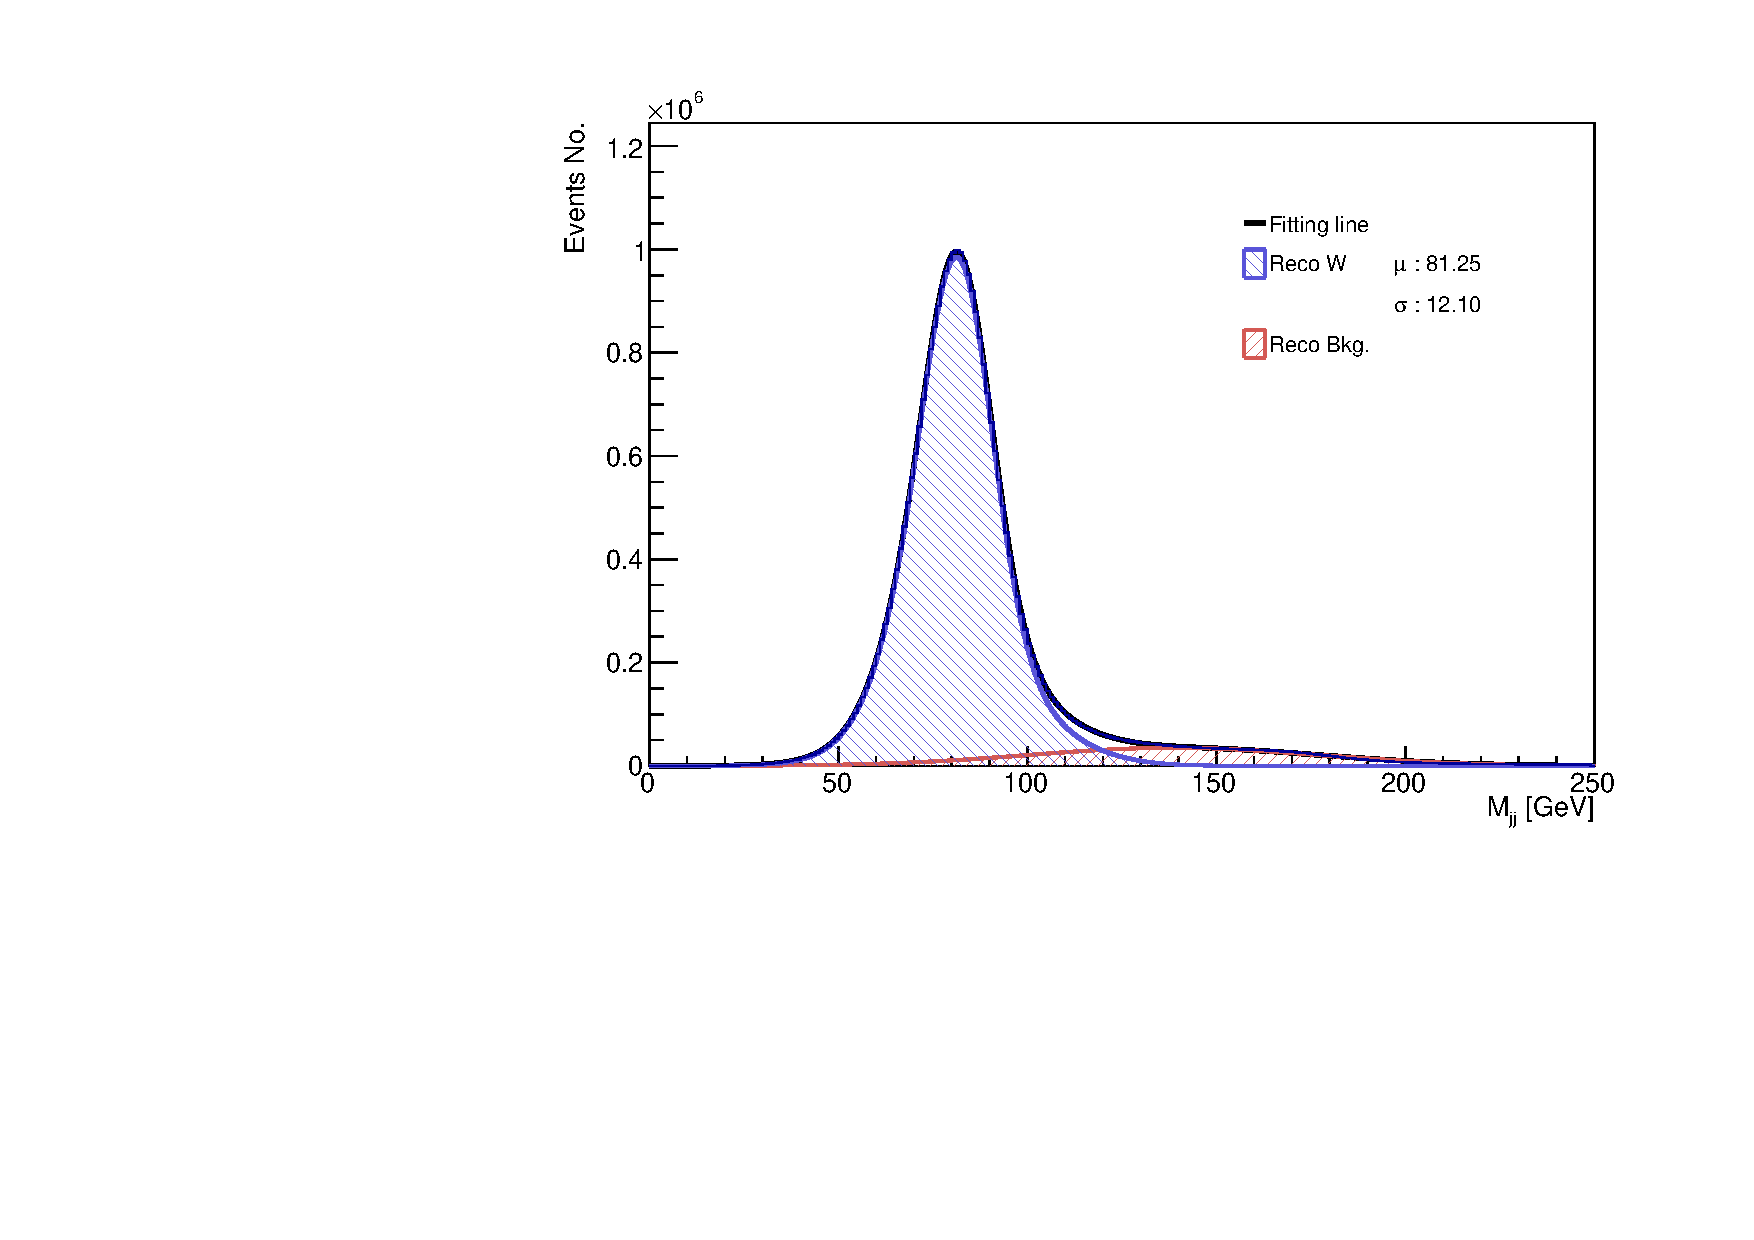
\includegraphics[width=0.45\textwidth]{Figures/EventSelReco/Fit/Plot_h_Mjj.pdf}}
			    \subfigure[Top quarks]{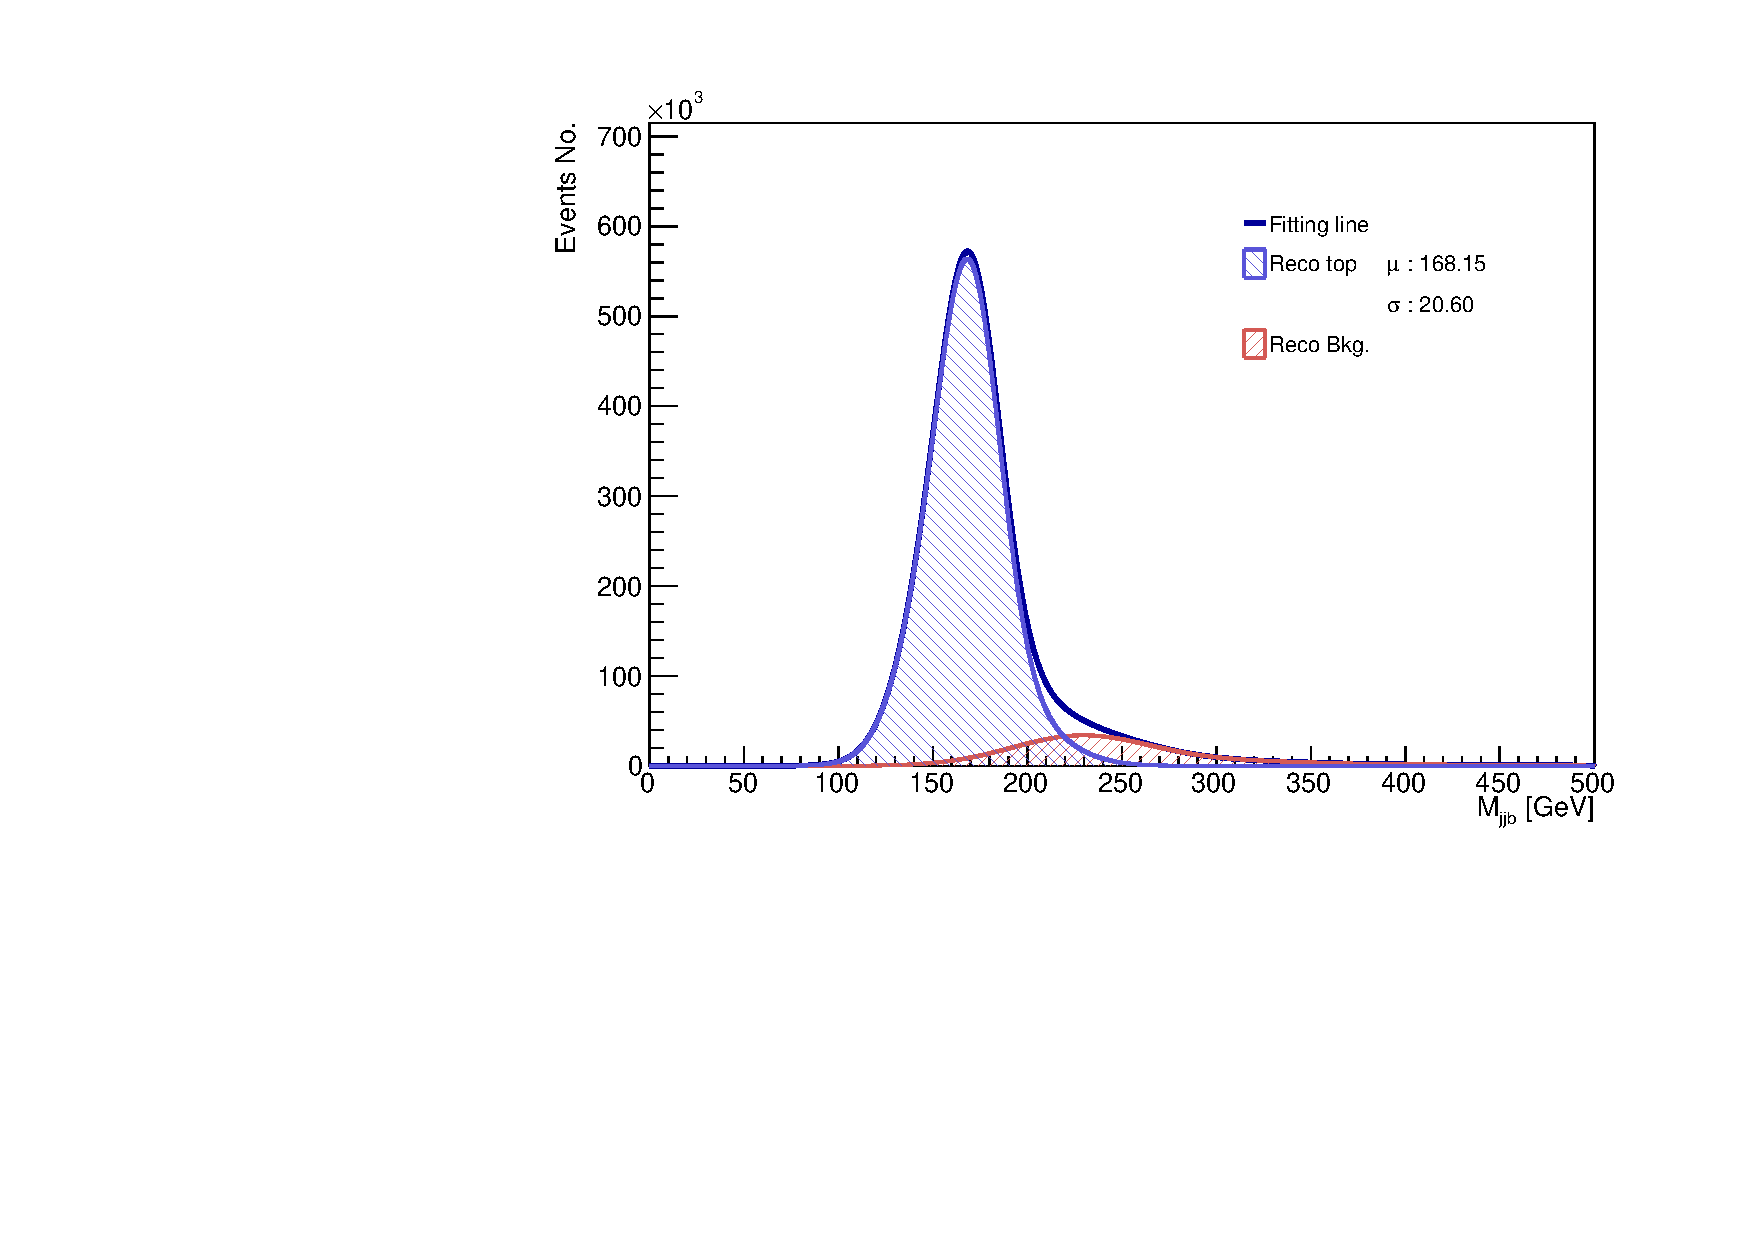
\includegraphics[width=0.45\textwidth]{Figures/EventSelReco/Fit/Plot_h_Mjjb.pdf}}\\
			\caption{The fitted results of top quark's and W boson's invariant mass for $\chi^2_{min}$ method}
			\label{EventSelReco:fig:fitted_mass}
			\end{figure}
			\FloatBarrier


			Back to the part of $\chi^2$, for each combination, $m_{jjb}$ is the invariant mass of 1 b-tagged jet and 2 non-btagged jets; $m_{jj}$ is the invariat mass of 2 non b-tagged jets which are same 2 jets in $m_{jjb}$. the combination who have the minimum ${\chi}^{2}$ value in all of them is chosen as physical obsects coming from hadronically decay top.


\begin{figure}[H]
\centering
	\subfigure[muon channel]{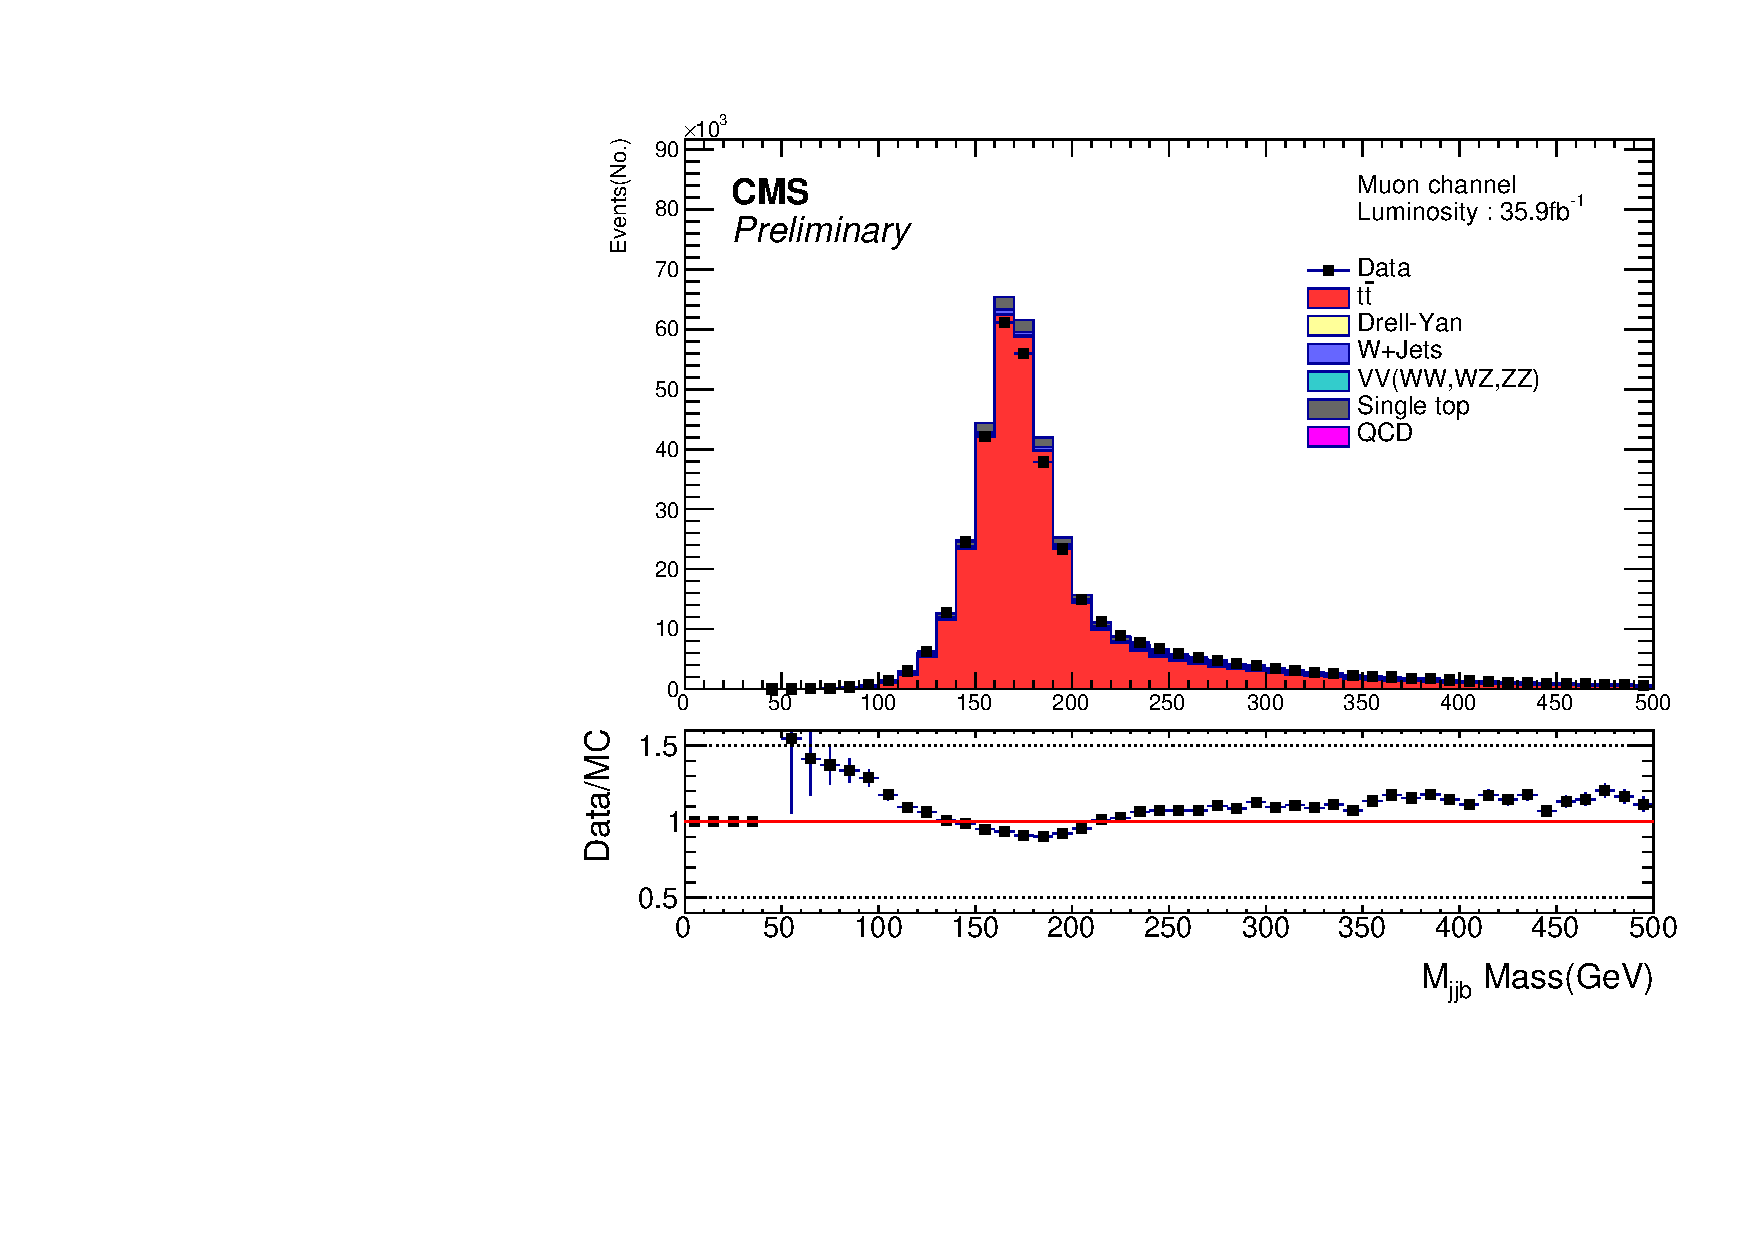
\includegraphics[width=0.45\textwidth]{Figures/EventSelReco/Mass/chi2/chi2_NC_long_HadTop_mu.pdf}}
    \subfigure[electron channel]{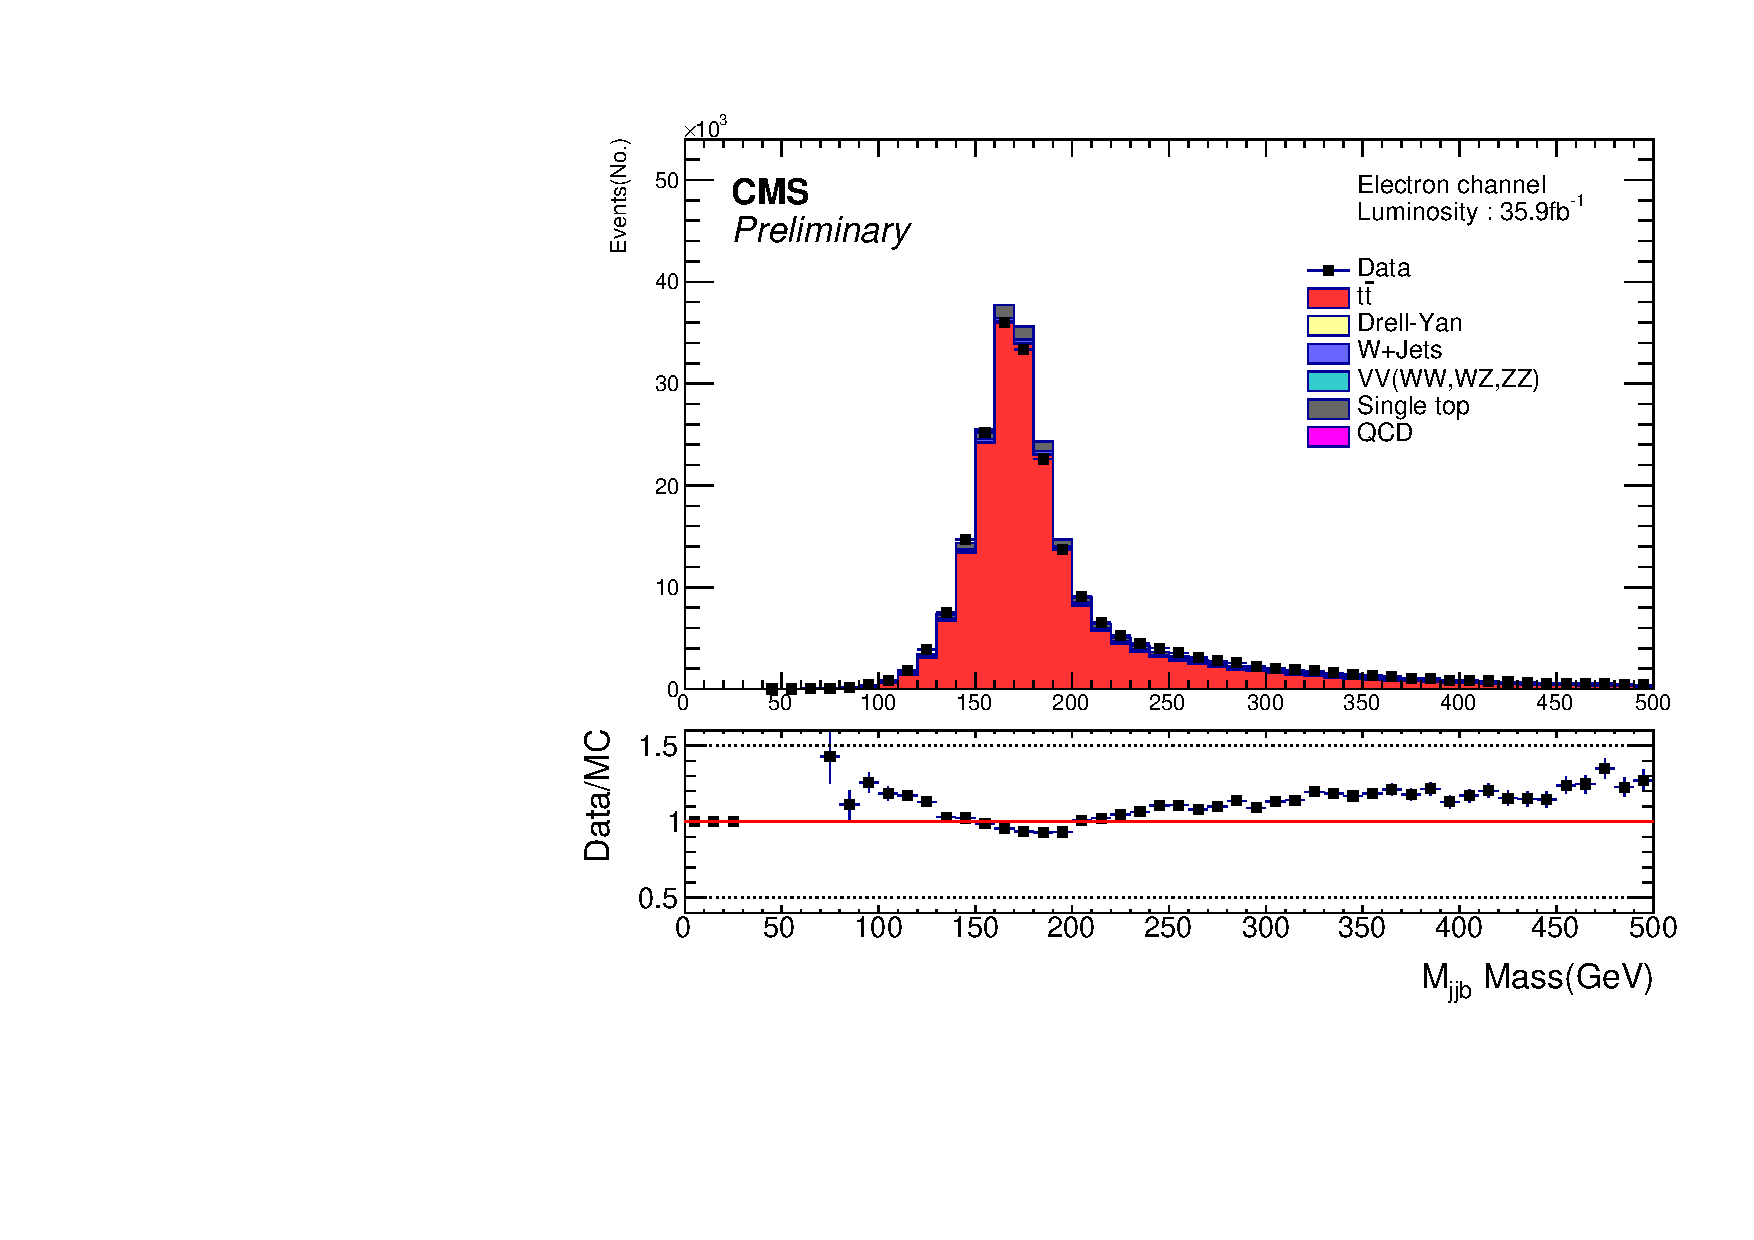
\includegraphics[width=0.45\textwidth]{Figures/EventSelReco/Mass/chi2/chi2_NC_long_HadTop_el.pdf}}\\
\caption{Reconstructed $M_{jjb}$ with $\chi^2_{min}$ algorithm (w/o cut)}
\label{EventSelReco:fig:chi2_SR_NC_Mjjb}
\end{figure}
\FloatBarrier

		\subsubsection{MVA Method}
		\label{sssec:mva_intro} 

			However, to improve the reconstruction performance in my analysis, there is another method - $\textbf{Multi-Variate Analysis (MVA)}$ can be adopted to do well in this reconstruction part. It has been not a common way to used in this step yet compared to signal and background samples' classification. In order to check the improvement between usual and new method, in the following rest analysis, the comparison of analysis results of $\chi^2_{min}$ method and MVA method will be shown simultaneously. 

			The concept of MVA is to use basic machine learning method to classify signal and background, we'll take advantage of MVA discriminating ability to improve the correctness rate of selection compared with $\chi^2_{min}$ method.
				
			As the usage of classification, one should define the $"$signal$"$ and $"$background$"$ in MVA configuration. In most particle physics analysis with MVA, $"$signal$"$ means the physics sample which is expected to be analyzed and as a target sample and the $"$background$"$ means samples from the other known physics. Different as usual, in this analysis,

			\begin{itemize}

				\item Sample : signal simulation sample($t\bar{t}$ MC) with full event selection(\ref{ssec:EvtSel_SR})
				\item Randomly half for training sample, another half for testing sample
				\item In each event,
				\begin{enumerate}
					\item $\textbf{Signal}$ is recognized as the correct combination of objects hadronically decaying from $t$($\bar{t}$)-quark in an event
					\item $\textbf{Background}$ are all the other incorrect combinations in an event
				\end{enumerate}
			\end{itemize}

			To identify whether one combination is the 2 jets and the correct detector-level's objects from generator-level's particles, the $\Delta R$ method is used to match them. The matching method is to compare the angle distribution between detector-level objects and generator-level particles with $\Delta R$ < 0.4. 
			
			\begin{equation}
			\Delta R = \sqrt{ (\eta_{det} - \eta_{gen})^2 - (\phi_{det} - \phi_{gen})^2 } < 0.4
			\label{eq:gen_matching}
			\end{equation}
		
			With concept of machine learning, we need to train with informations of classes( $"$signal$"$ and $"$backgroud$"$ in this case ) and get out an algorithm to make distinguishment. Following the original $\chi^2_{min}$ method's variables, we started MVA with inputting 2 variables : $m_{jj}$, $m_{jjb}$, as informations to be used for distinguishment. There are three machine learning methods I used for testing: $\textbf{MLP}$(ANN, Artificial Neuro-Network), $\textbf{BDT}$(Boosted Decision Tree), $\textbf{BDTG}$(Boosted Decision Tree Gradient).

			For these three algorithm to do the training, there are some algorithms' parameter setting for them individually:

			\begin{itemize}

				\item $\textbf{BDT}$ :
				\begin{enumerate}
					\item Number of trees in the forest : 800
					\item Max depth of the decision tree allowed : 3
				\end{enumerate}
				\item $\textbf{BDTG}$ :
				\begin{enumerate}
					\item Number of trees in the forest : 800
					\item Minimum percentage of training events required in a leaf node : 2.5\%
					\item Boosting type for the trees in the forest : GradBoost
					\item Learning rate for GradBoost algoithm : 0.10
					\item Use only a random subsample of all events for growing the trees in each iteration (only for GradBoost) : True
					\item Relative size of bagged event sample to original size of the data sample (used whenever bagging is used) : 0.5
					\item Number of grid points in variable range used in finding optimal cut in node splitting : 20
					\item Max depth of the decision tree allowed : 3
				\end{enumerate}
				\item $\textbf{MLP}$ :
				\begin{enumerate}
					\item Variable transformations : type N
					\item Neuron activation function type : sigmoid function
					\item Number of training cycles : 550
					\item Specification of hidden layer architecture : N, N+5, 3
					\item Test for overtraining performed at each $\#$th epochs : 5
					\item Use regulator to avoid overtraining : False
				\end{enumerate}
			\end{itemize}

			With respect to the input variables for distinguishment training, we can check the separation shows on input variables originally in advance:

			\begin{figure}[H]
			\centering{}
    			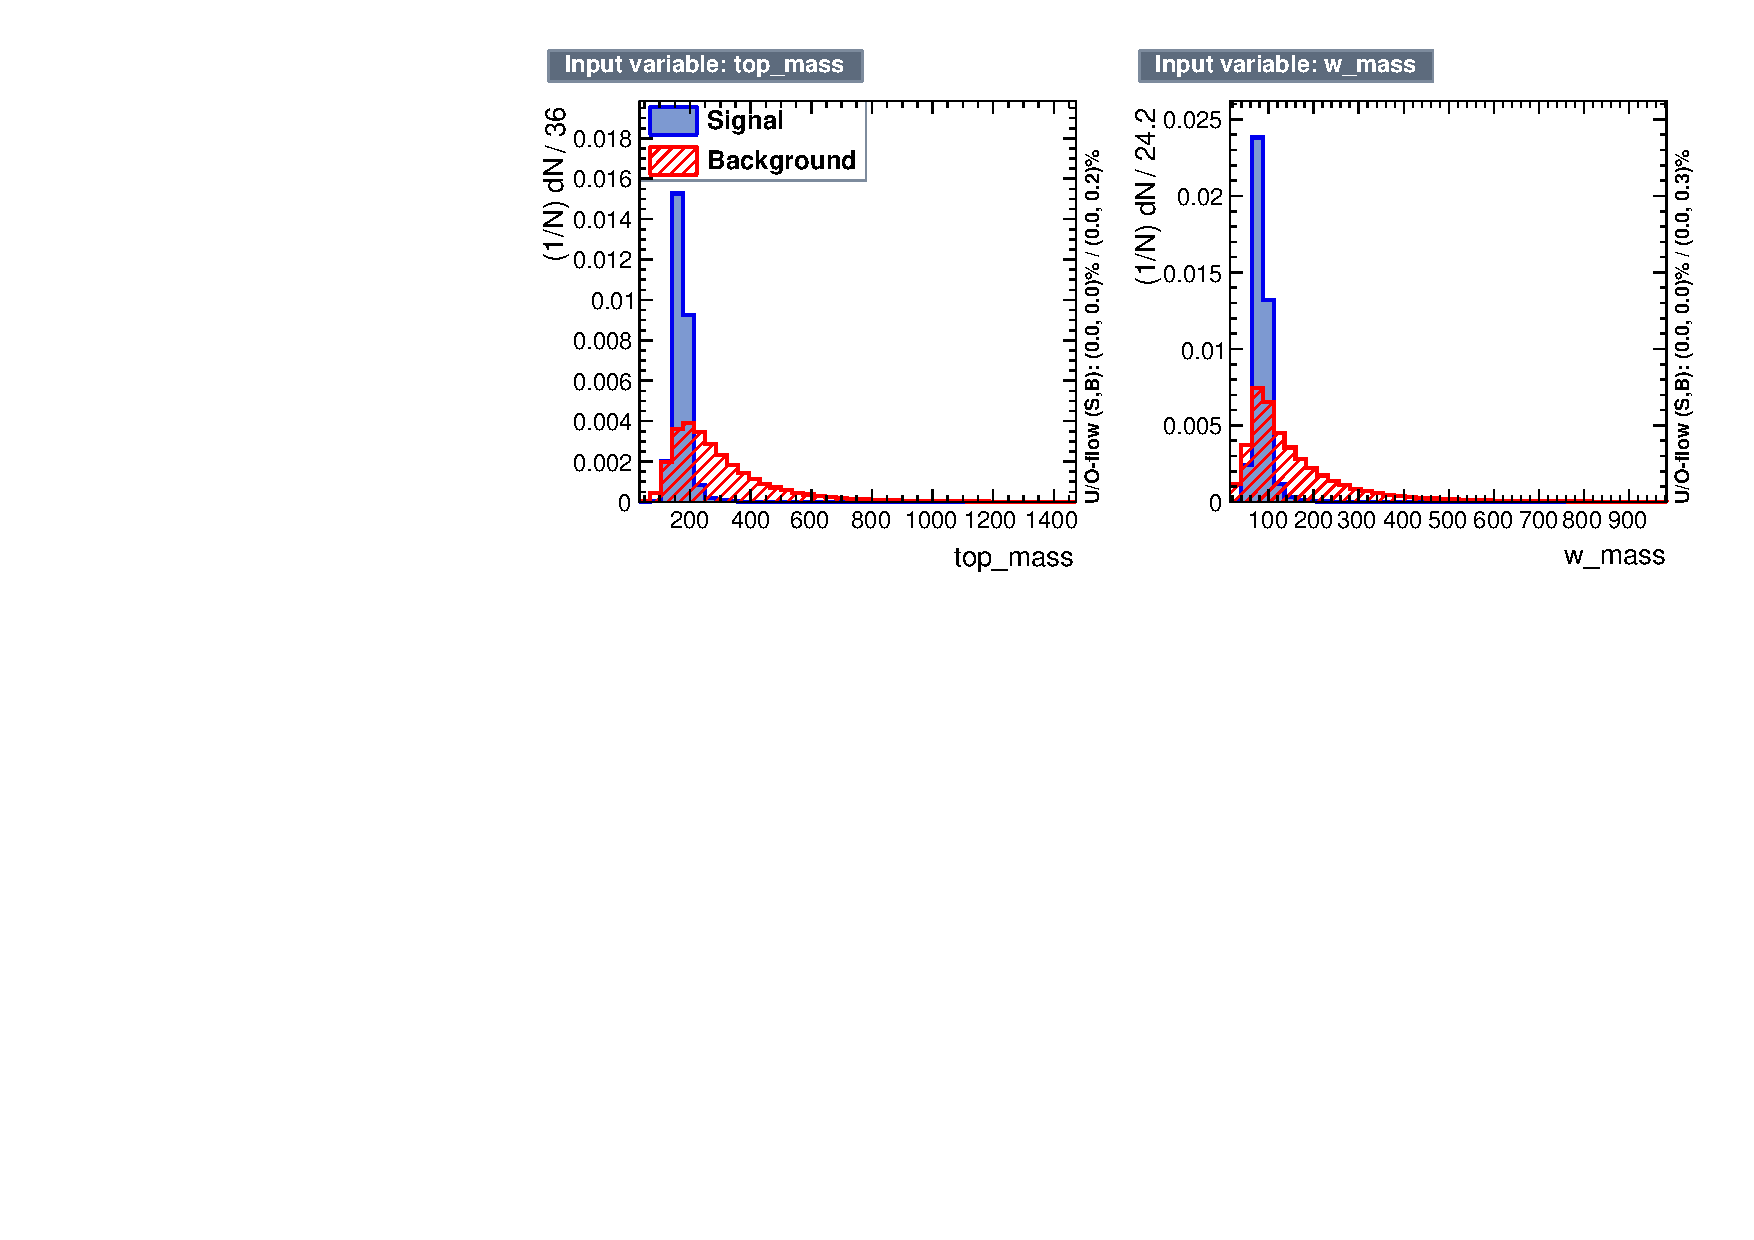
\includegraphics[width=0.85\textwidth]{Figures/EventSelReco/mva/a04_VarSep.pdf}\\
			\caption{Input training variables separation between $"$signal$"$ and $"$background$"$.(2 variables)}
			\label{EventSelReco:fig:a04_varsep}
			\end{figure}
			\FloatBarrier

			And the training result shows below:

			\begin{figure}[H]
			\centering
				\subfigure[BDT's separation result]{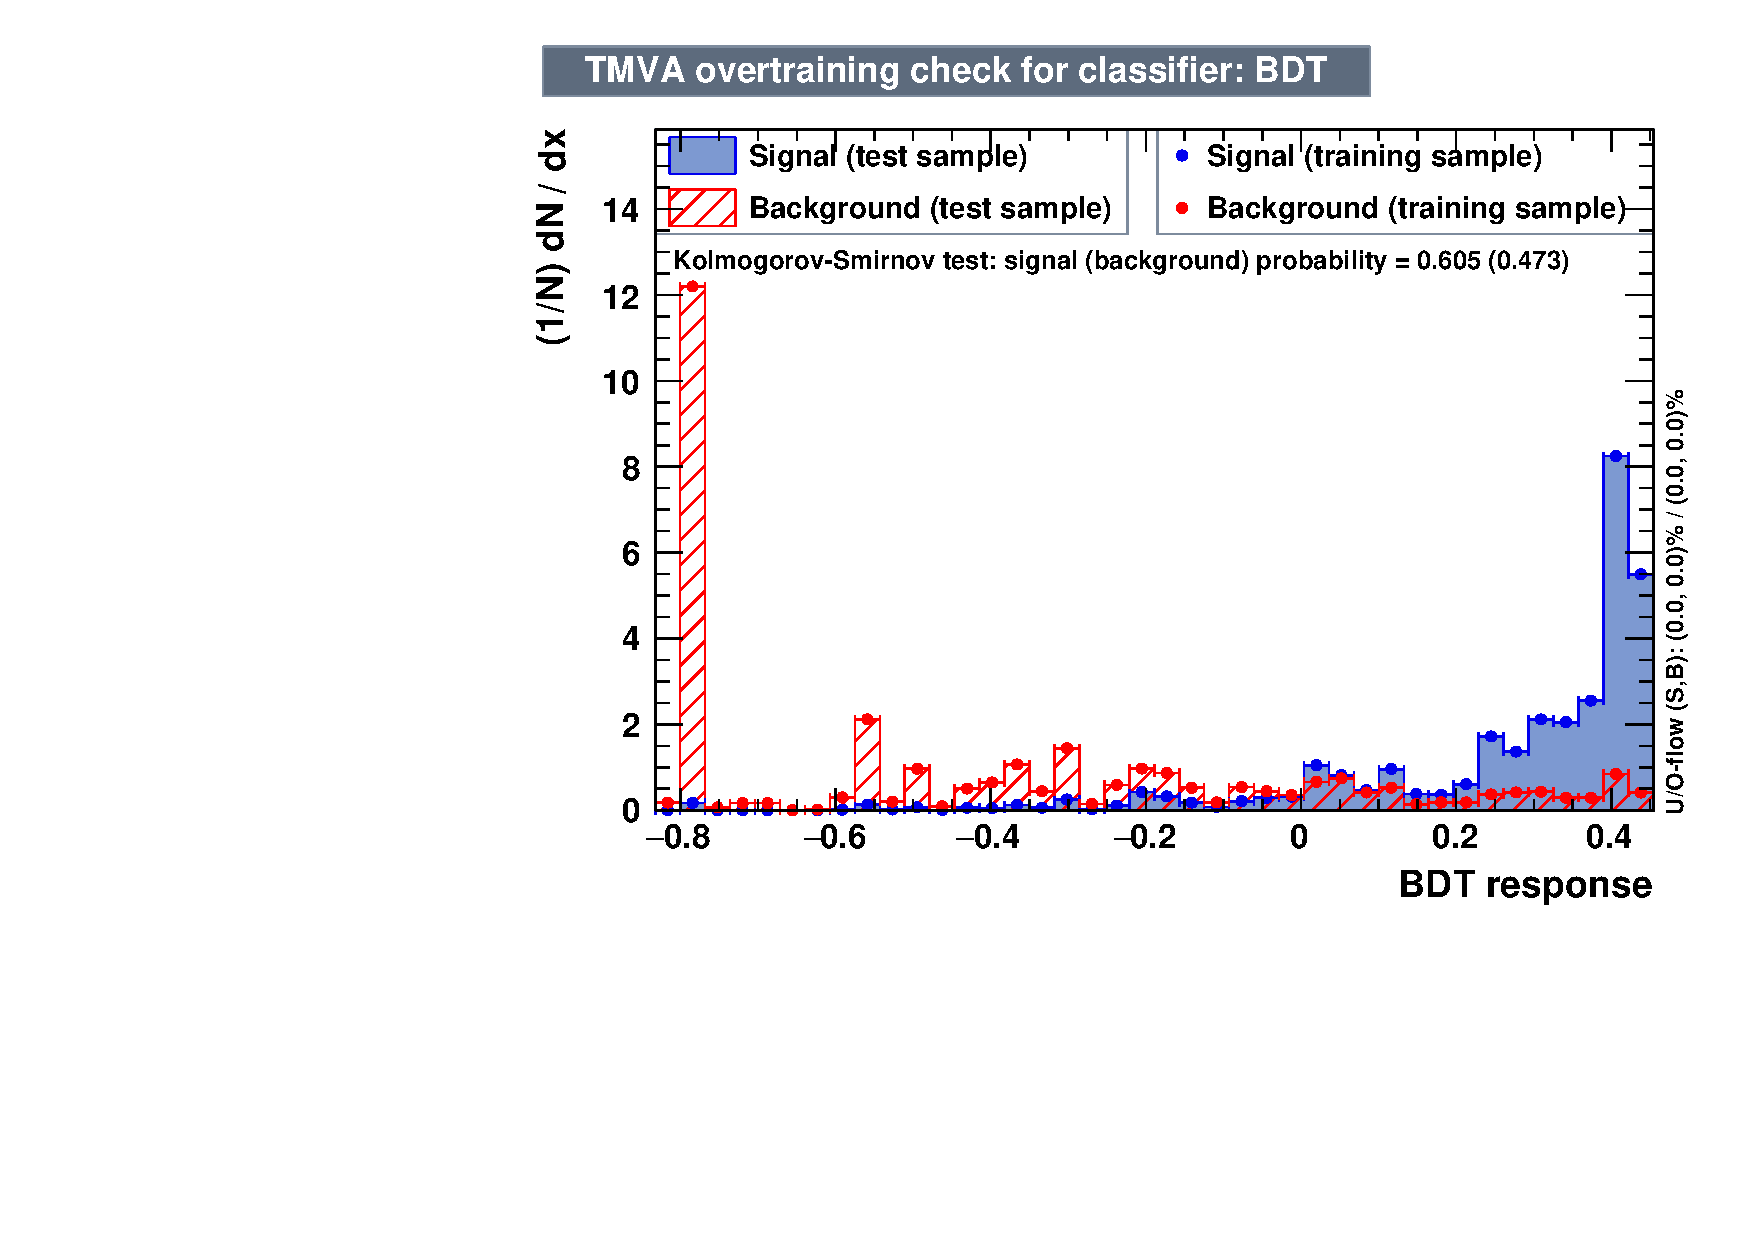
\includegraphics[width=0.45\textwidth]{Figures/EventSelReco/mva/a04_all_BDT_sep.pdf}}
			    \subfigure[BDTG's separation result]{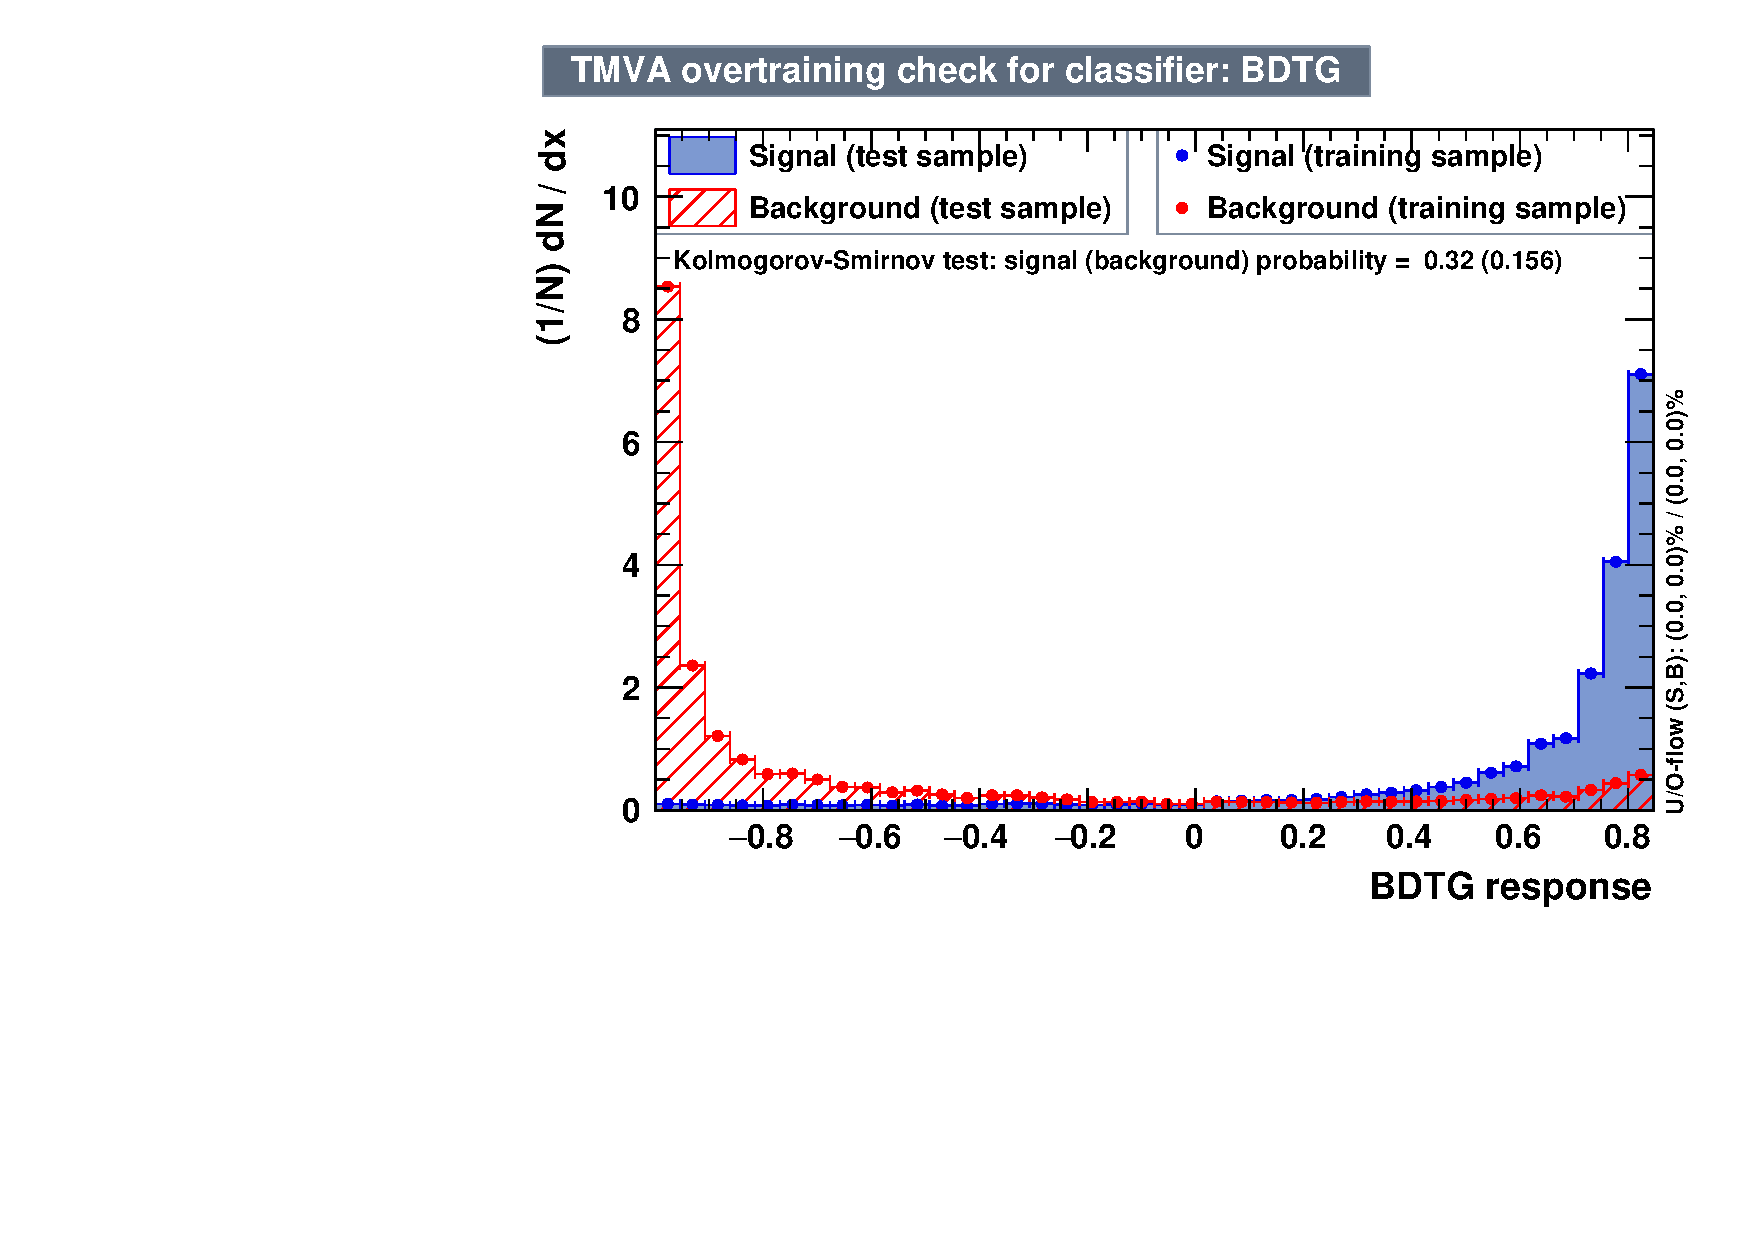
\includegraphics[width=0.45\textwidth]{Figures/EventSelReco/mva/a04_all_BDTG_sep.pdf}}\\
			    \subfigure[MLP's separation result]{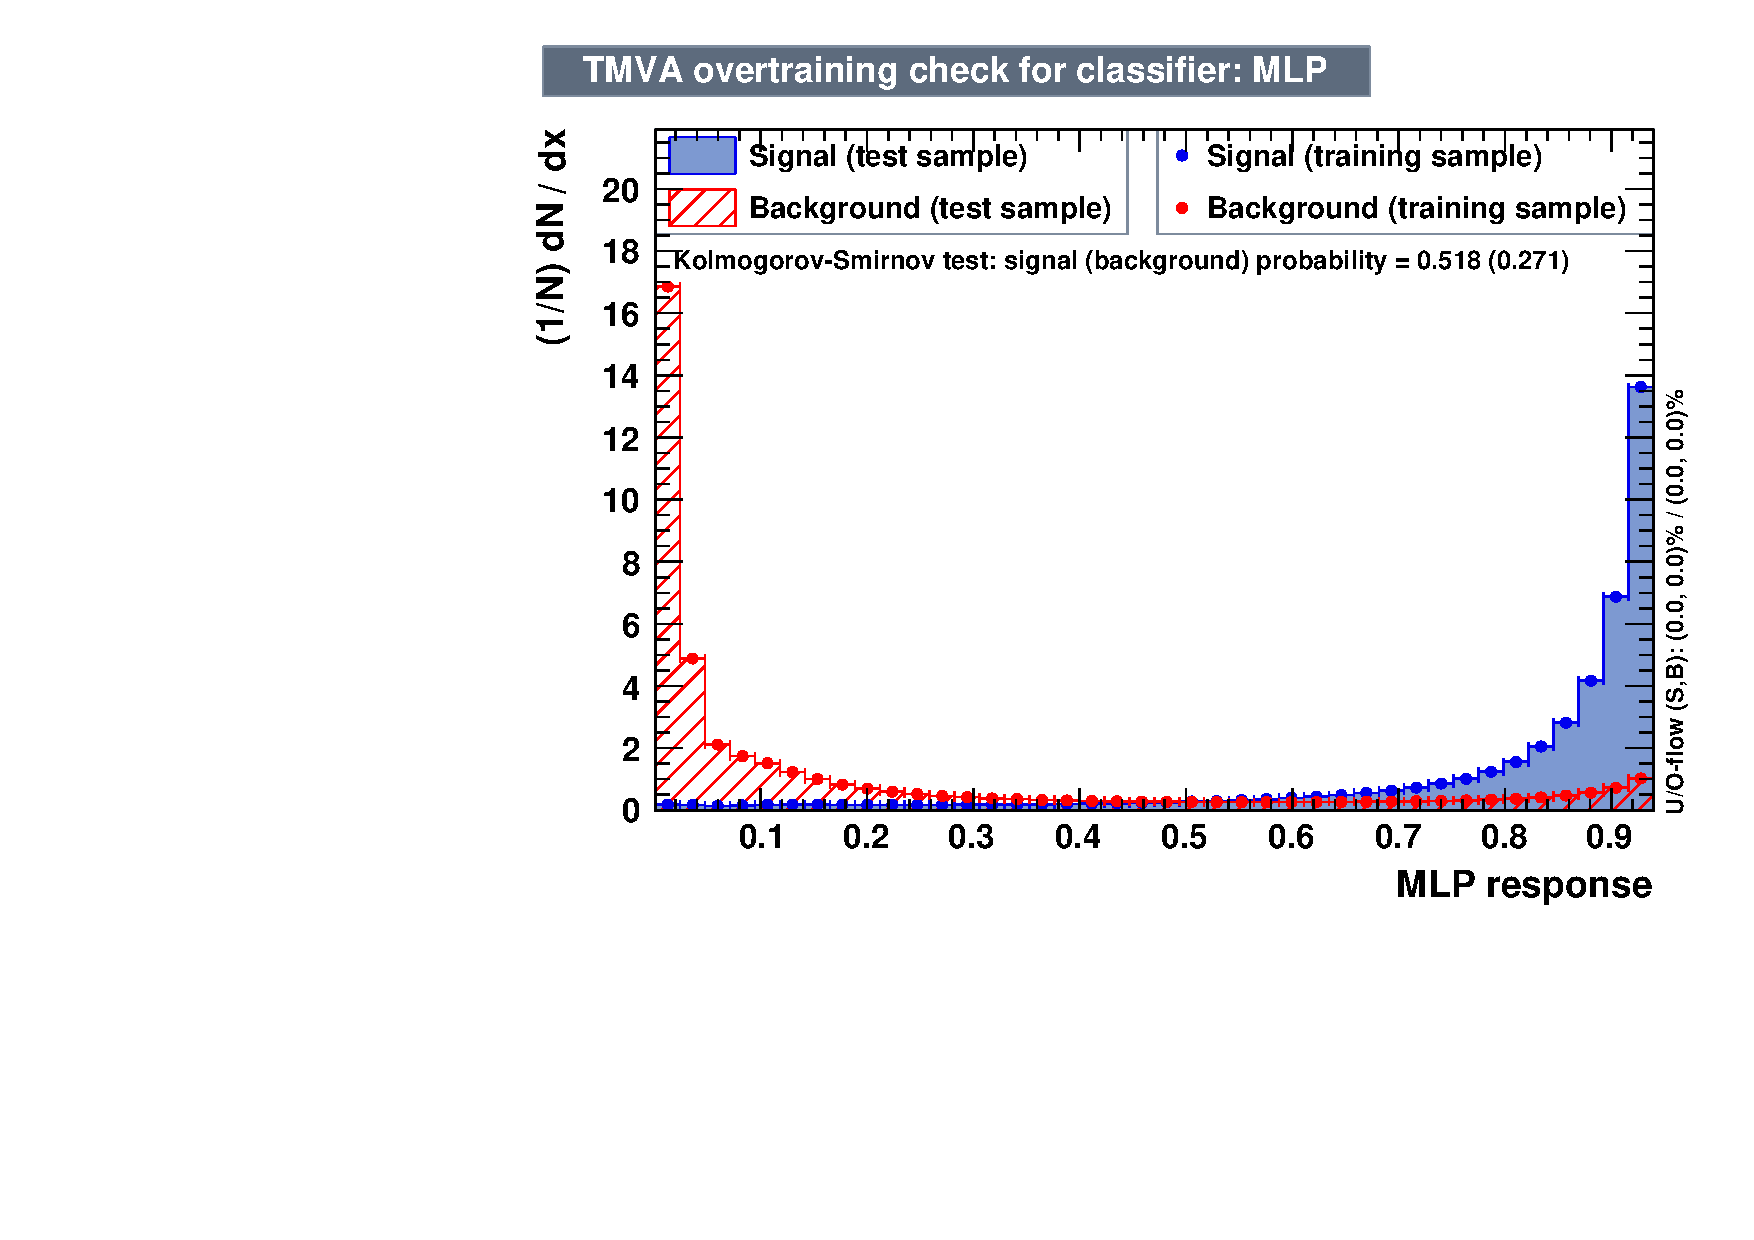
\includegraphics[width=0.45\textwidth]{Figures/EventSelReco/mva/a04_all_MLP_sep.pdf}}\\
			\caption{The separating distribution on signal and background}
			\label{EventSelReco:fig:Sep_a04}
			\end{figure}
			\FloatBarrier

			The separation plots Fig.\ref{EventSelReco:fig:Sep_a04} shows the machine learning methods' separating ability through the input training variables. The distributions in these plots are the final separation performance between $"$signal$"$ and $"$background$"$(right and wrong objects combination) with the training values which is propagated from separations of all input variables(Fig.\ref{EventSelReco:fig:a04_varsep}). It is also the separation performance under training sample and testing sample with given machine learning method. As we can see that if we want to pick out $"$signal$"$(right combination), just choose the jjb combination who has the $\emph{highist MVA score}$ as the right one.

			\begin{figure}[H]
			\centering{}
			    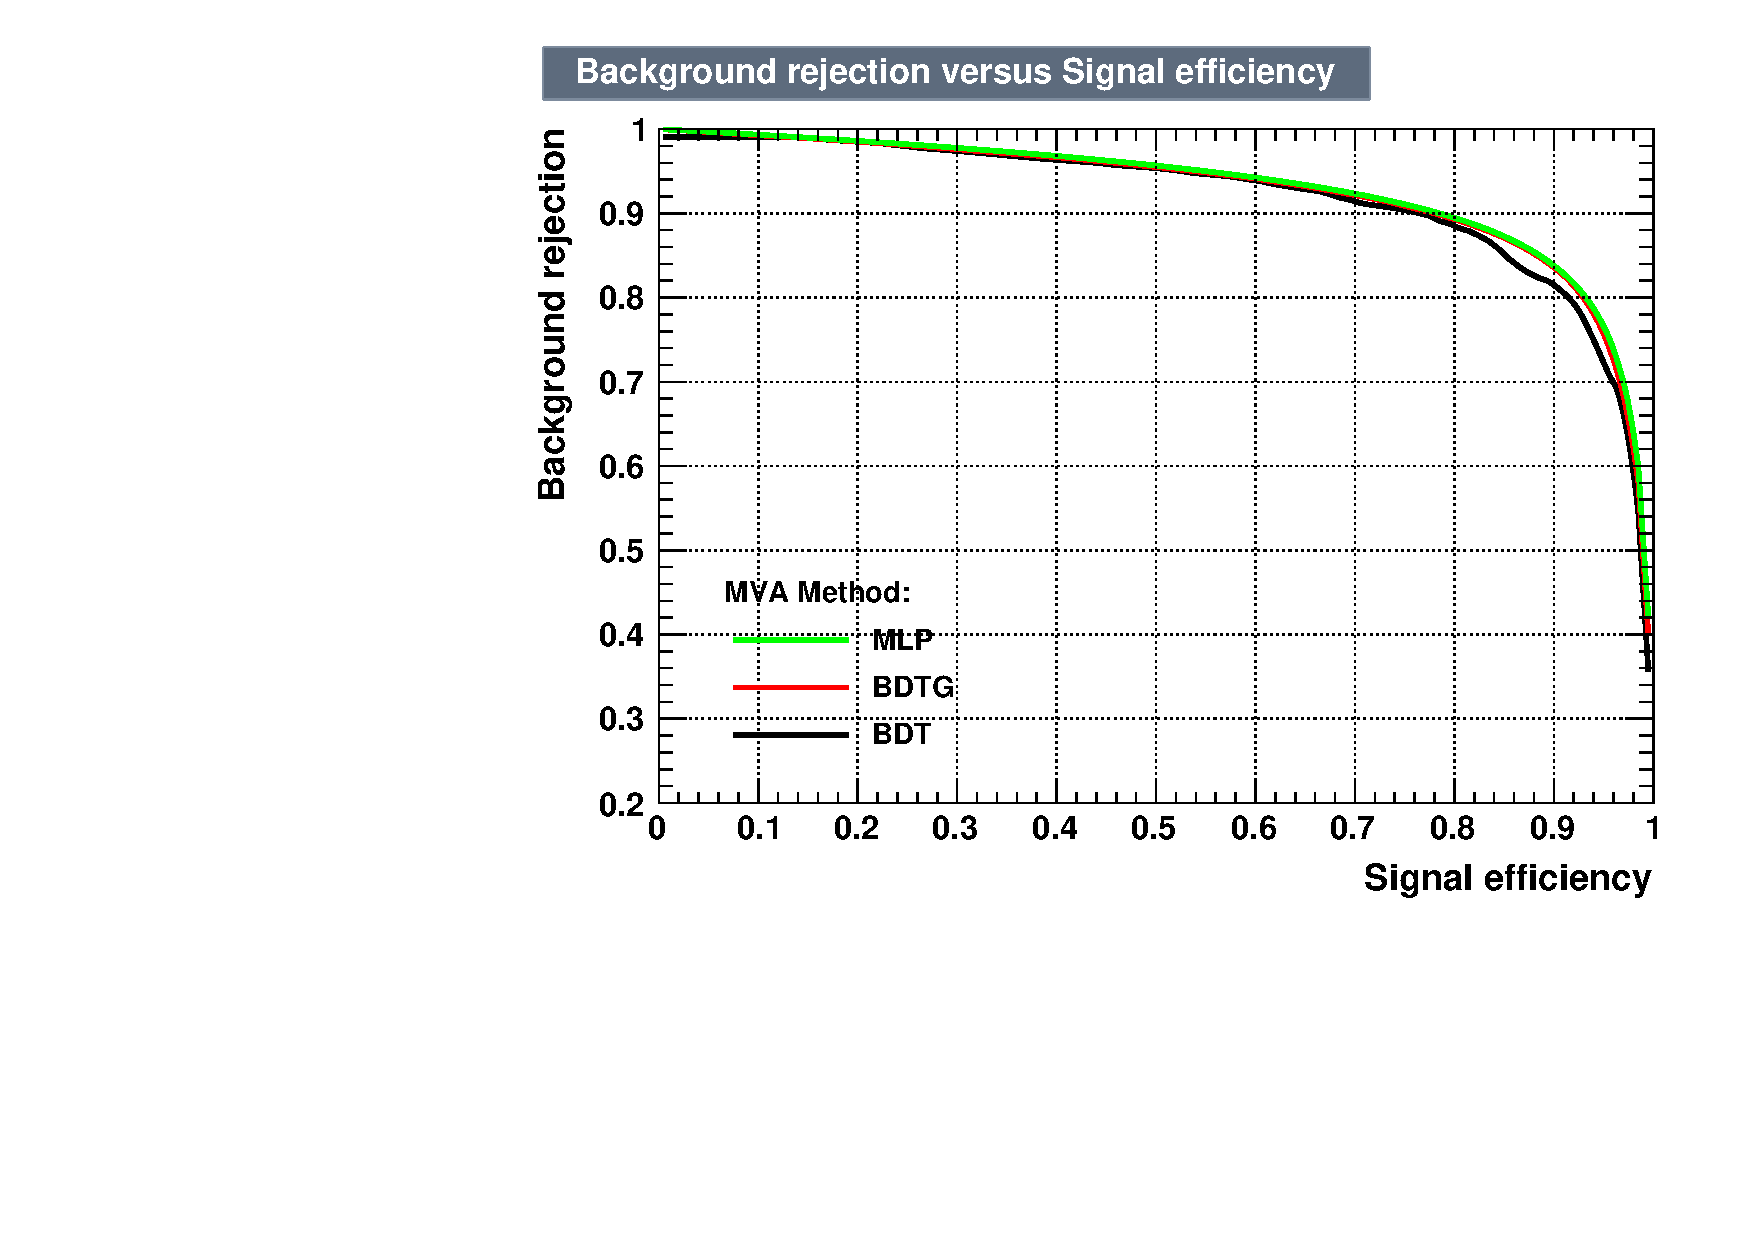
\includegraphics[width=0.6\textwidth]{Figures/EventSelReco/mva/a04_all_ROC.pdf}\\
			\caption{Receiver Operating Characteristic(ROC) curve of various machine learning method}
			\label{EventSelReco:fig:ROC_a04}
			\end{figure}
			\FloatBarrier
	
			The $\textbf{Receiver Operating Characteristic(ROC)}$ curve plot Fig.\ref{EventSelReco:fig:ROC_a04} can tell if it's given a cut on the output MVA score in separation distribution Fig.\ref{EventSelReco:fig:Sep_a04} to extract the $"$signal$"$, how the background rejection ratio vary when signal efficiency change. It can be infered that, the good performance is that when one rejects more ratio of background and at the same time reserves more ratio of signal(high signal efficiency). In other words, the bigger area under the ROC curve, the better the method is. However, the previous ROC criterion are just available and meaningful for the common case - one use MVA to separate the 2 different physics sample which are independent to each other, for example, use MVA to separate sigle $t$ and $t\bar{t}$ sample. In this analysis case, the signal and background are not separate like that kind in common. Being not independent 2 samples, signal and background are at the same time in one event instead. There are couple of complicated correlation between them. Therefore, the separation and ROC plots are not really fair anymore. As they going to not to be relative directly, there must be a standard to tell how MVA perform(That is the $b\bar{b}$ separation in \ref{ssec:bbsep}).

			There are also the reconstructed $M_{jjb}$ with MVA algorithm.($m_{jjb}$, $m_{jj}$) There is just MLP (instead of BDT/BDTG)results shown here.

			\begin{figure}[H]
			\centering
				\subfigure[muon channel]{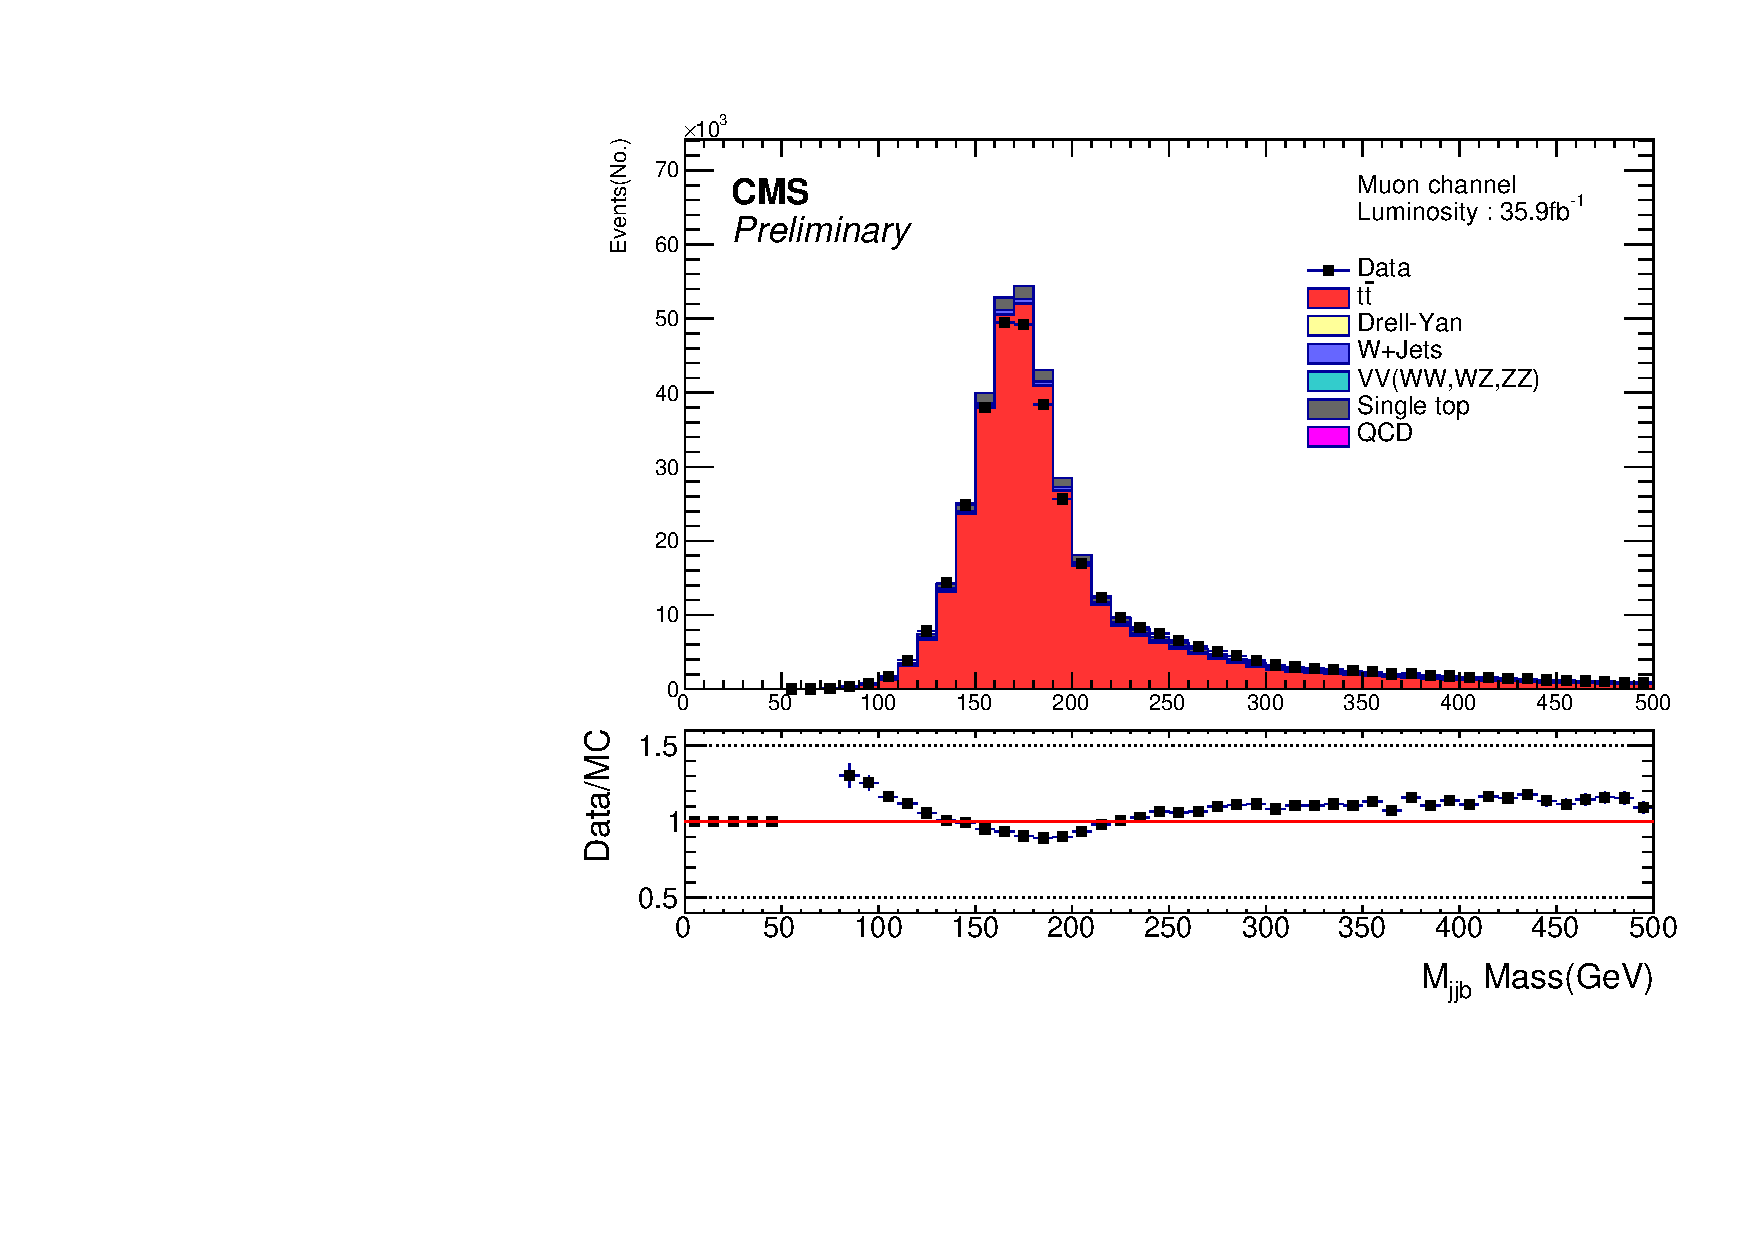
\includegraphics[width=0.45\textwidth]{Figures/EventSelReco/Mass/a04/a04_MLP_NC_long_HadTop_mu.pdf}}
			    \subfigure[electron channel]{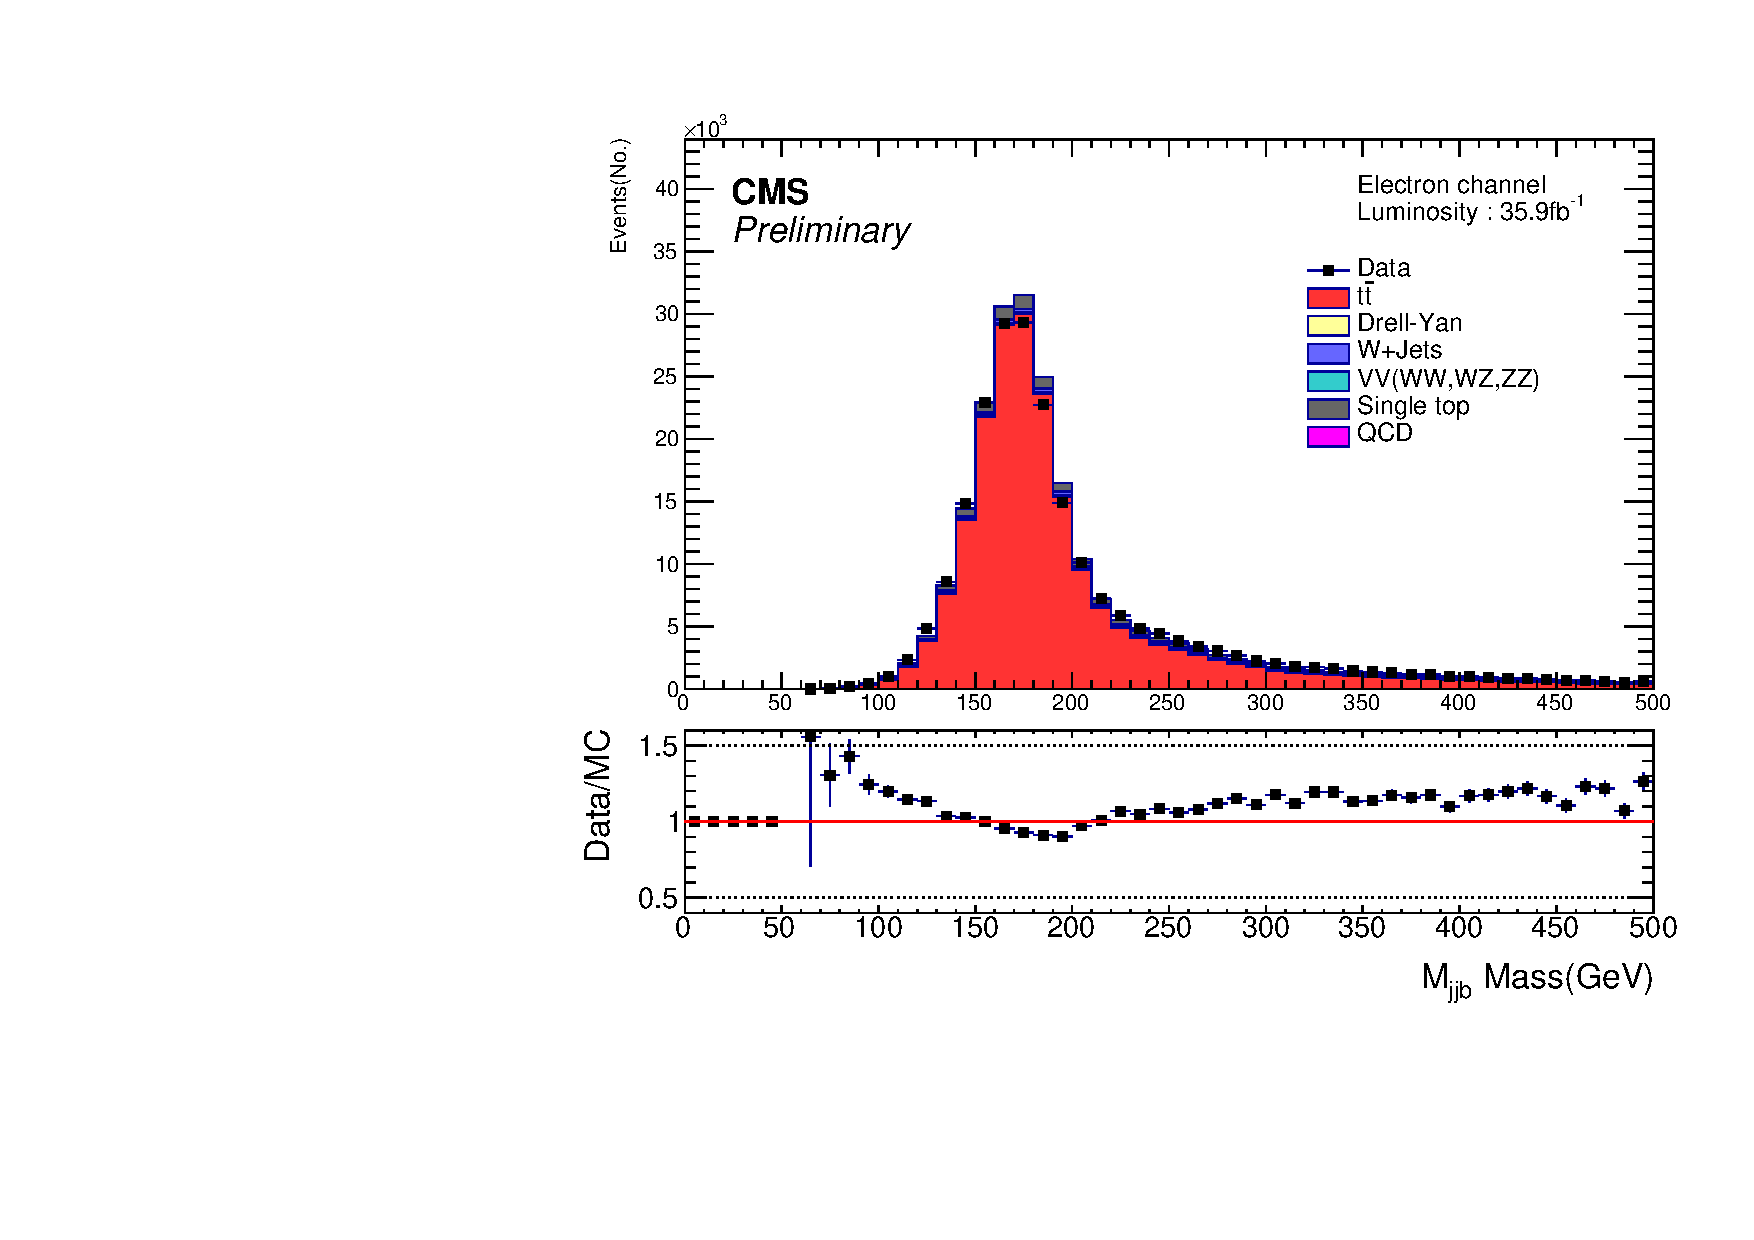
\includegraphics[width=0.45\textwidth]{Figures/EventSelReco/Mass/a04/a04_MLP_NC_long_HadTop_el.pdf}}\\
			\caption{Reconstructed $M_{jjb}$ with 2 variables MLP algorithm (w/o cut)}
			\label{EventSelReco:fig:a04_MLP_SR_NC_Mjjb}
			\end{figure}
			\FloatBarrier

			And also, it is better to use MVA with more variables than just $m_{jj}$ and $m_{jjb}$. There are 3 variables sets after a bunch of trials here to input and train. It's a remindful item that they are the variables of each combination in any event.

			\begin{enumerate}
			\item The first set: (2 variables)
				\begin{itemize}
				\item $m_{jjb}$, $m_{jj}$
				\end{itemize}

			%%% TODO: this set need to be eliminate before showing the result of bbsep performance
			\item The second set: (8 variables)
				\begin{itemize}
				\item $m_{jjb}$, $m_{jj}$
				\item 2 jets'(jj) $\sum P_{T}$, $\Delta \phi$, $\Delta \eta$
				\item selected lepton and leptonic b-jet's $\sum P_{T}$, $\Delta \phi$, $\Delta \eta$ 
				\end{itemize}

			\item The third set: (20 variables)
				\begin{itemize}
				\item $m_{jjb}$, $m_{jj}$
				\item 2 jets'(jj) $\sum P_{T}$, $|\Delta P_{T}|$, $\Delta R$
				\item hadronic W(j+j) and hadronic b-jet's $\sum P_{T}$, $|\Delta P_{T}|$, $\Delta R$
				\item selected lepton and hadronic b-jet's $\sum P_{T}$, $|\Delta P_{T}|$, $\Delta R$
				\item selected lepton and hadronic W(j+j)'s $\sum P_{T}$, $|\Delta P_{T}|$, $\Delta R$
				\item hadronic W(j+j) and MET's $\sum P_{T}$, $|\Delta P_{T}|$, $\Delta \phi$
				\item hadronic b-jet and MET's $\sum P_{T}$, $|\Delta P_{T}|$, $\Delta \phi$
				\end{itemize}
			\label{EventSelReco:itm:mva_var}
			\end{enumerate}

			Besides the training result of the 2 variables' set have been shown(Fig.\ref{EventSelReco:fig:a04_varsep}, Fig.\ref{EventSelReco:fig:Sep_a04}, Fig.\ref{EventSelReco:fig:ROC_a04}), there are also the training results of 8 variables and 20 variables' cases:

			\begin{figure}[H]
			\centering{}
    			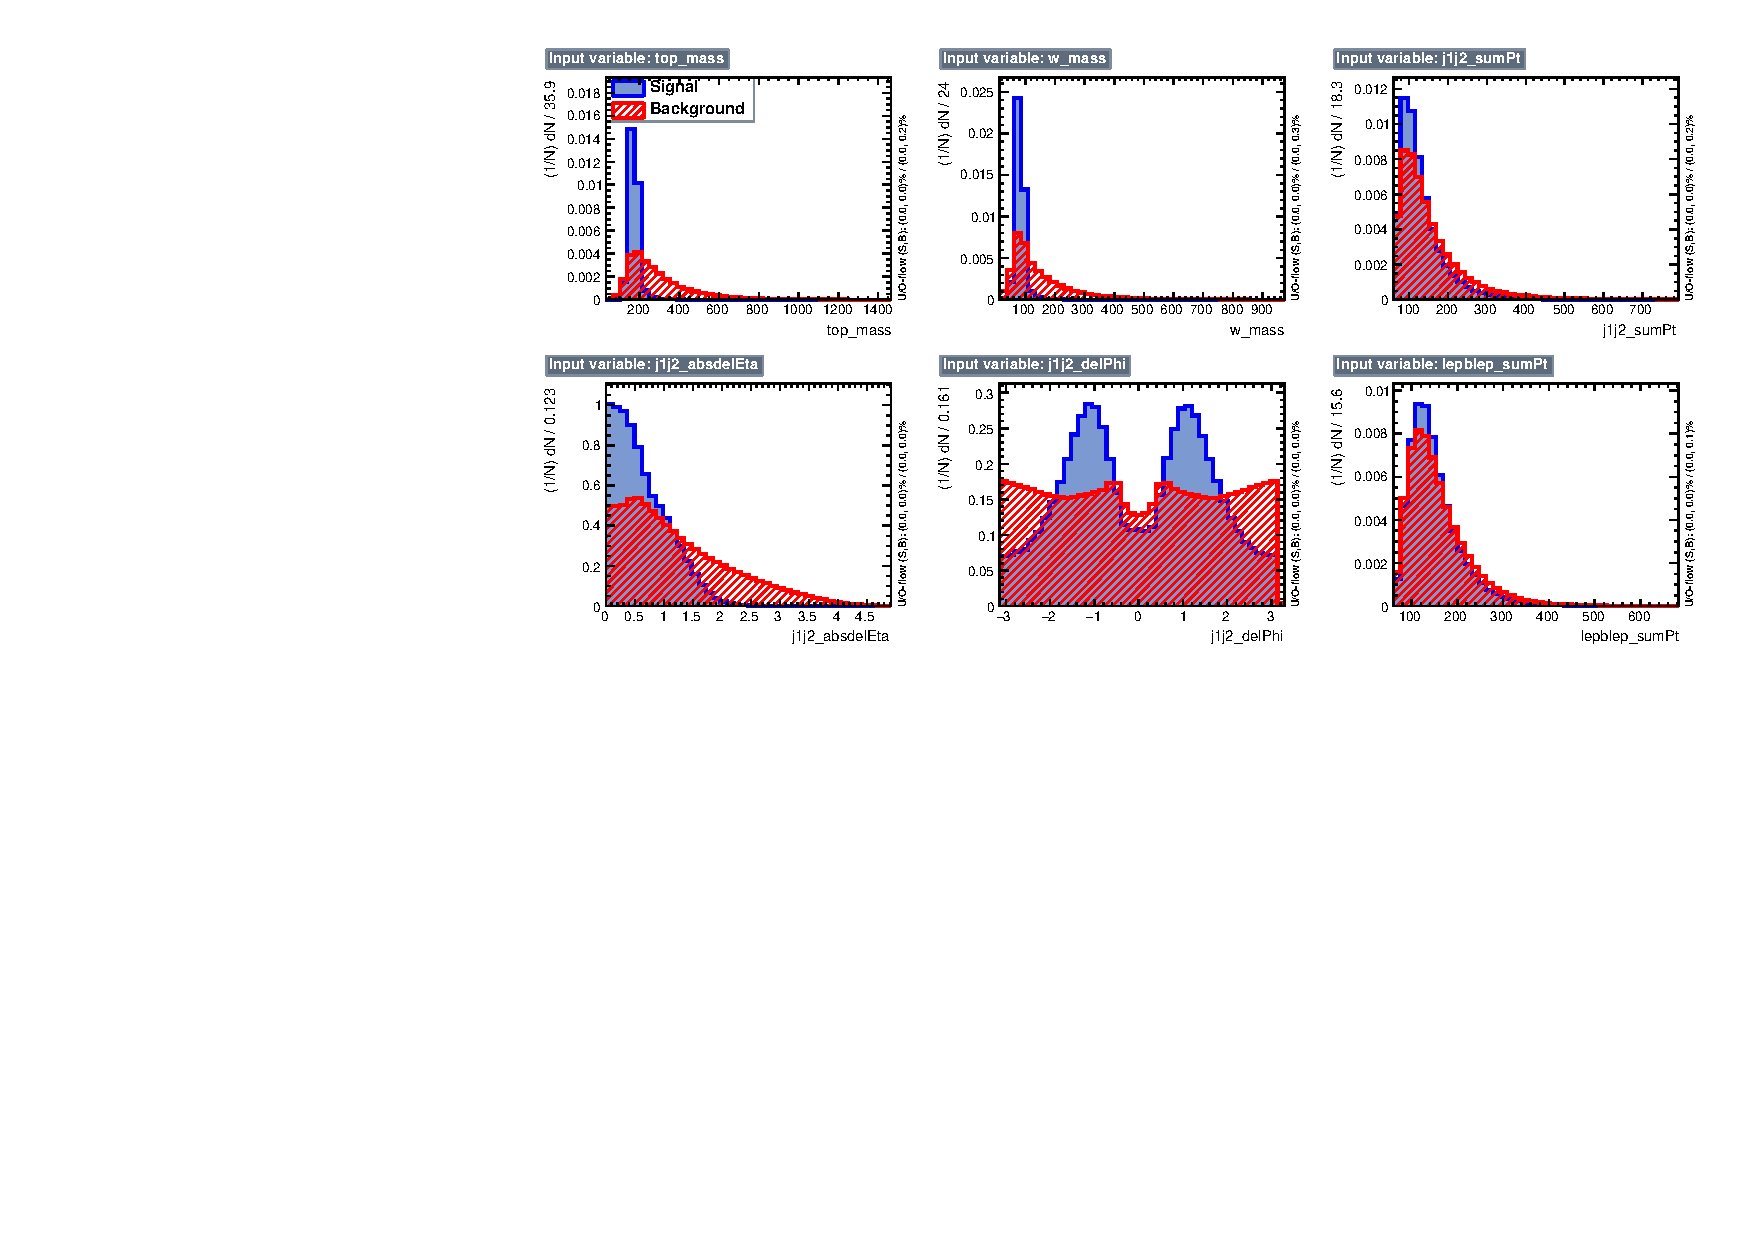
\includegraphics[width=0.8\textwidth]{Figures/EventSelReco/mva/t13_VarSep1.pdf}\\
			\end{figure}
			\FloatBarrier
			\begin{figure}[H]
			\centering{}
    			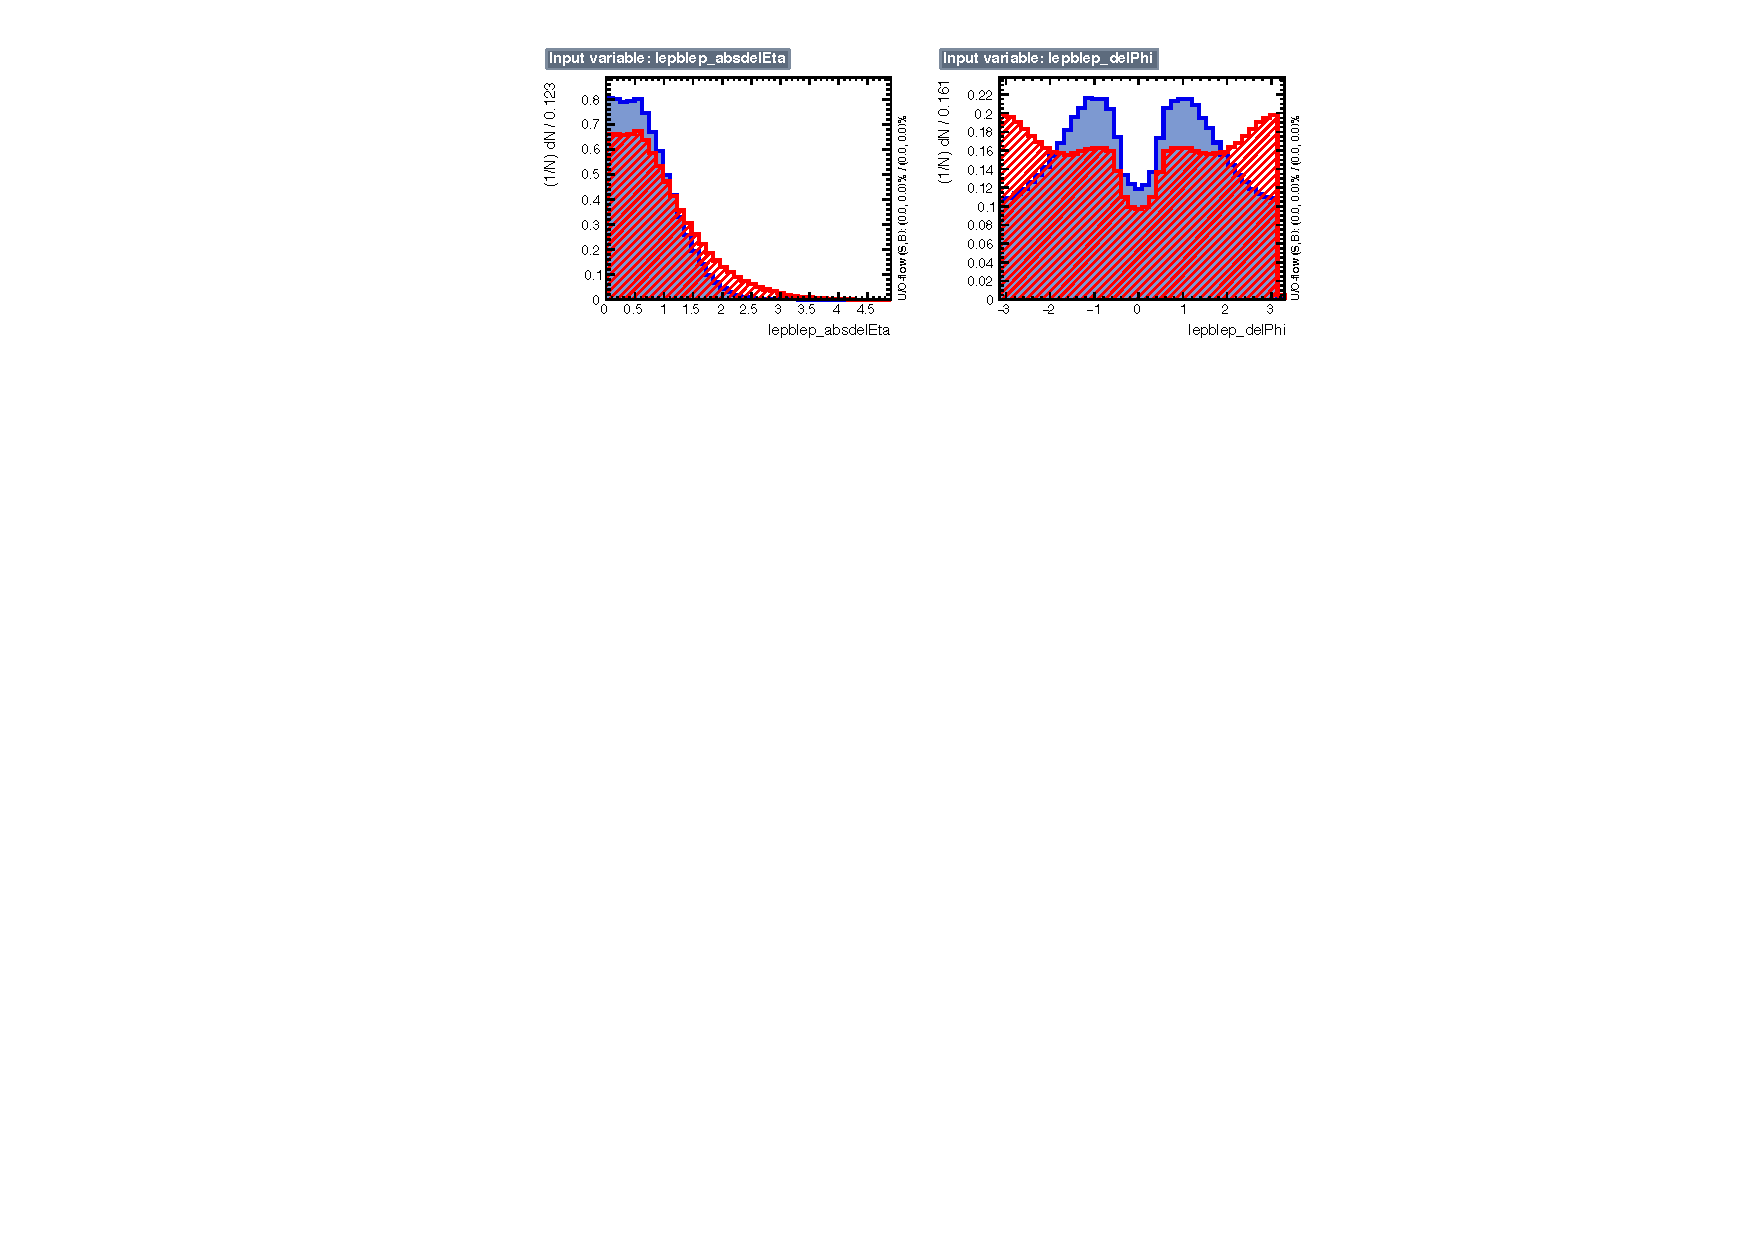
\includegraphics[width=0.528\textwidth]{Figures/EventSelReco/mva/t13_VarSep2.pdf}\\
    		\caption{Input training variables separation between $"$signal$"$ and $"$background$"$.(8 variables)}
			\label{EventSelReco:fig:t13_varsep}
			\end{figure}
			\FloatBarrier

			\begin{figure}[H]
			\centering
				\subfigure[BDT's separation result (8 vars)]{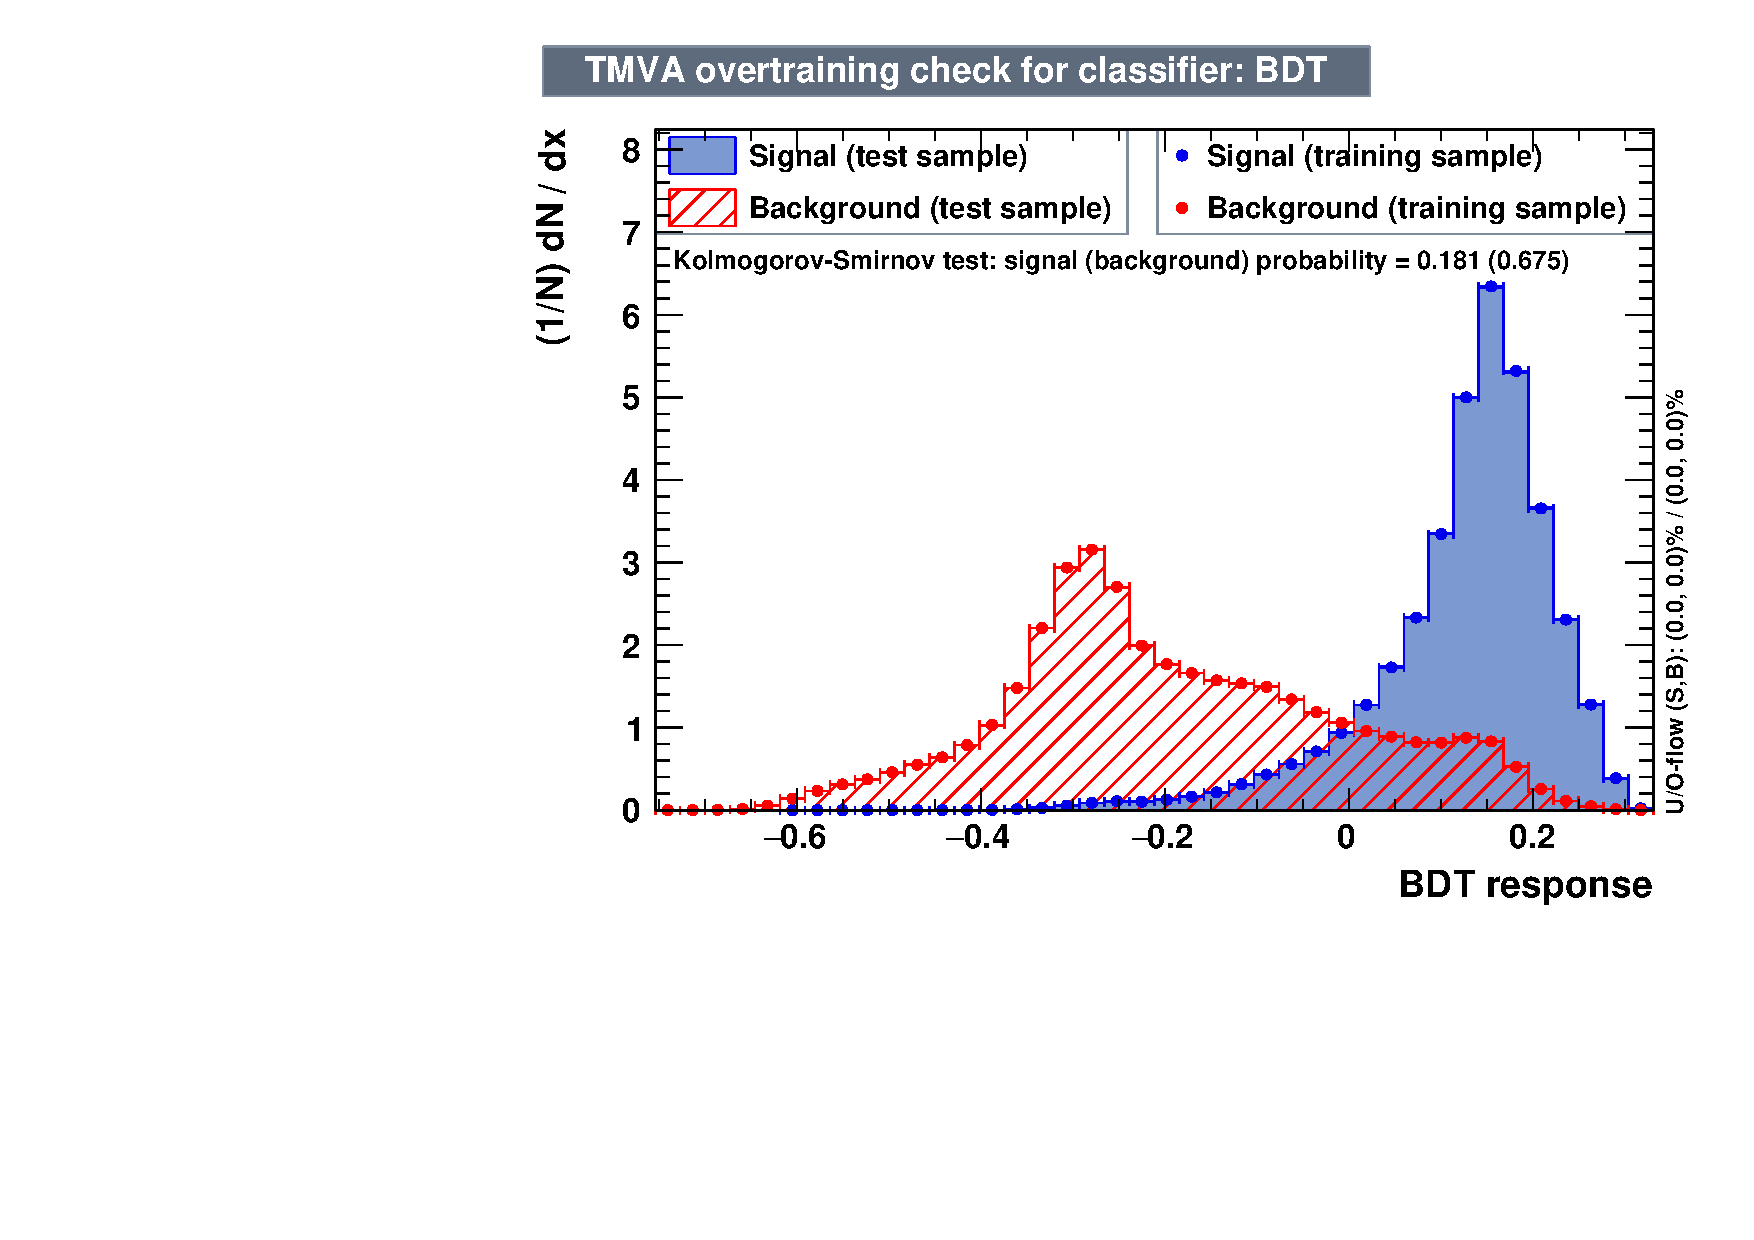
\includegraphics[width=0.4\textwidth]{Figures/EventSelReco/mva/t13_BDT_sep.pdf}}
			    \subfigure[BDTG's separation result (8 vars)]{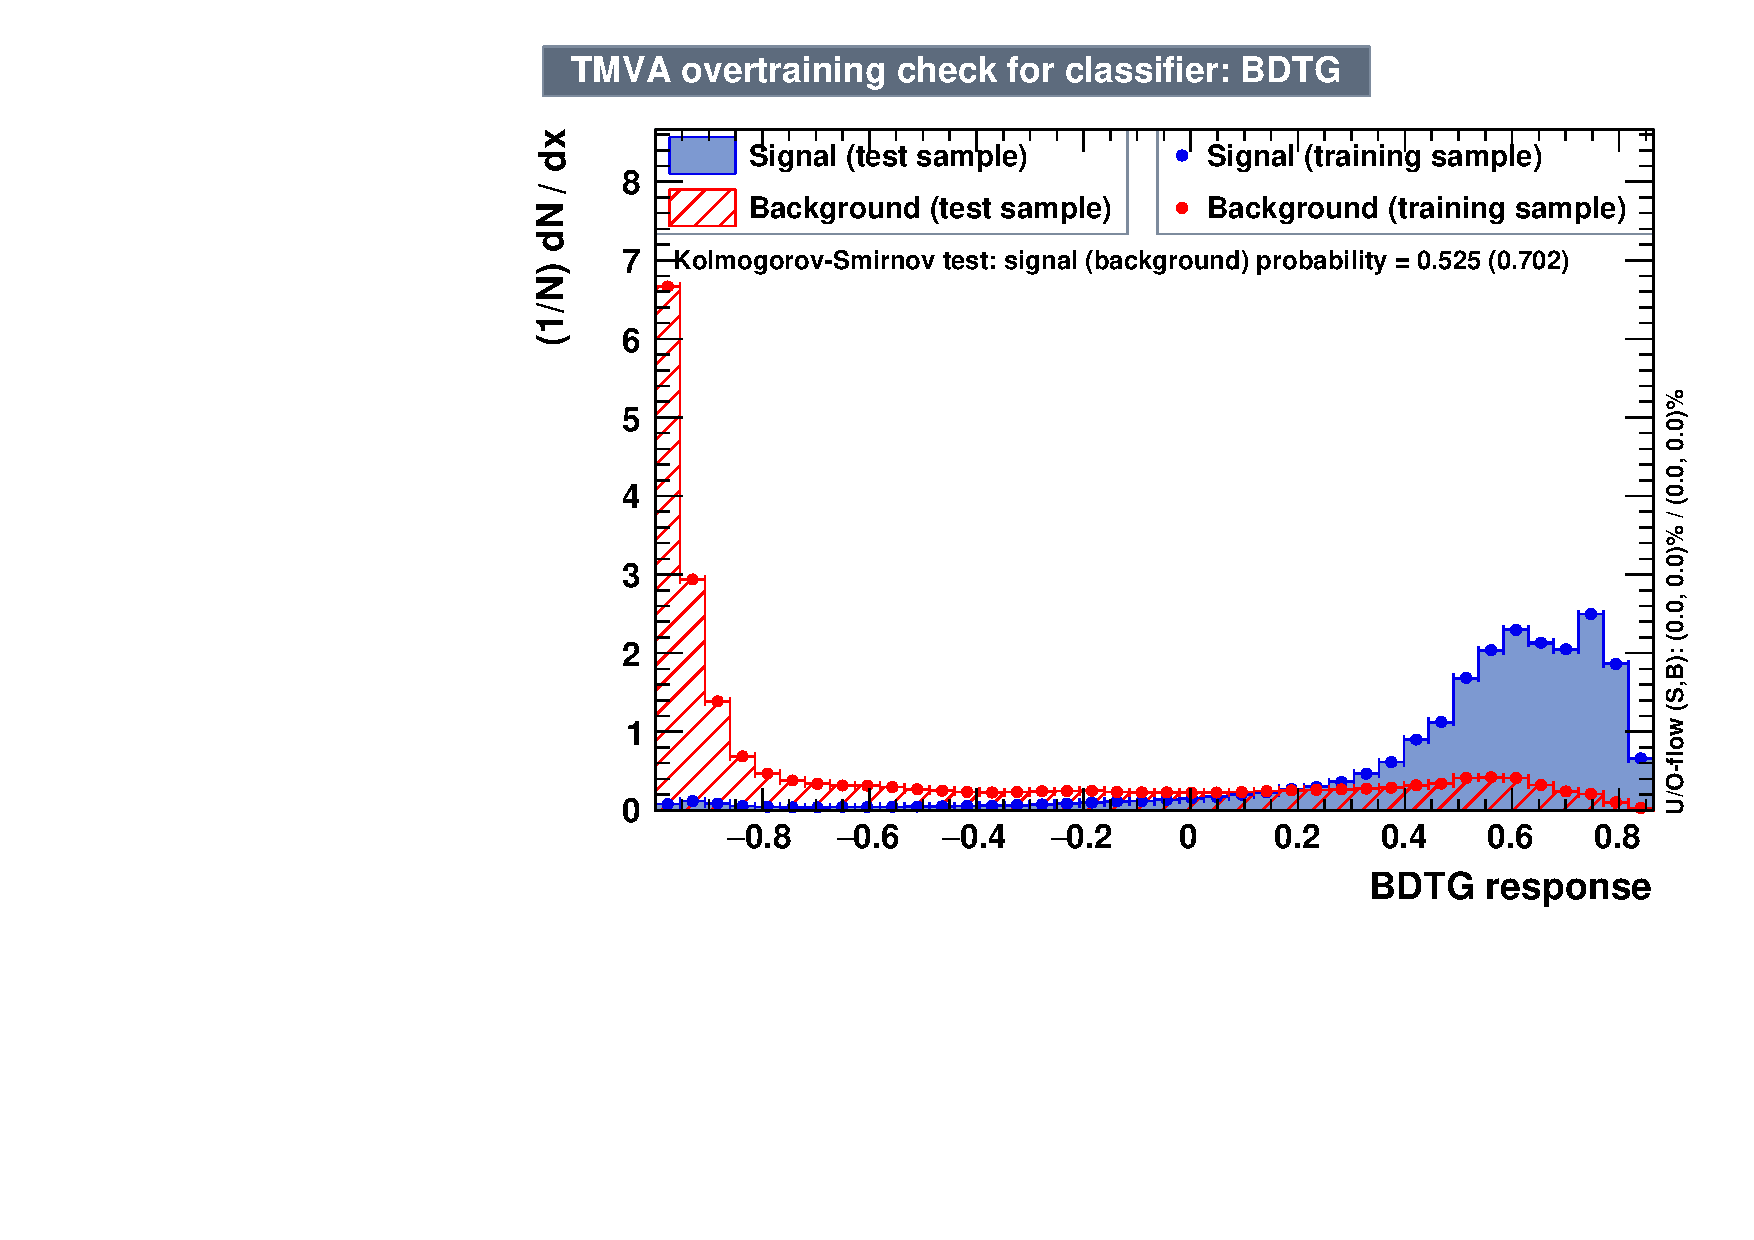
\includegraphics[width=0.4\textwidth]{Figures/EventSelReco/mva/t13_BDTG_sep.pdf}}\\
			\end{figure}
			\FloatBarrier
			\begin{figure}[H]
			\centering
			    \subfigure[MLP's separation result (8 vars)]{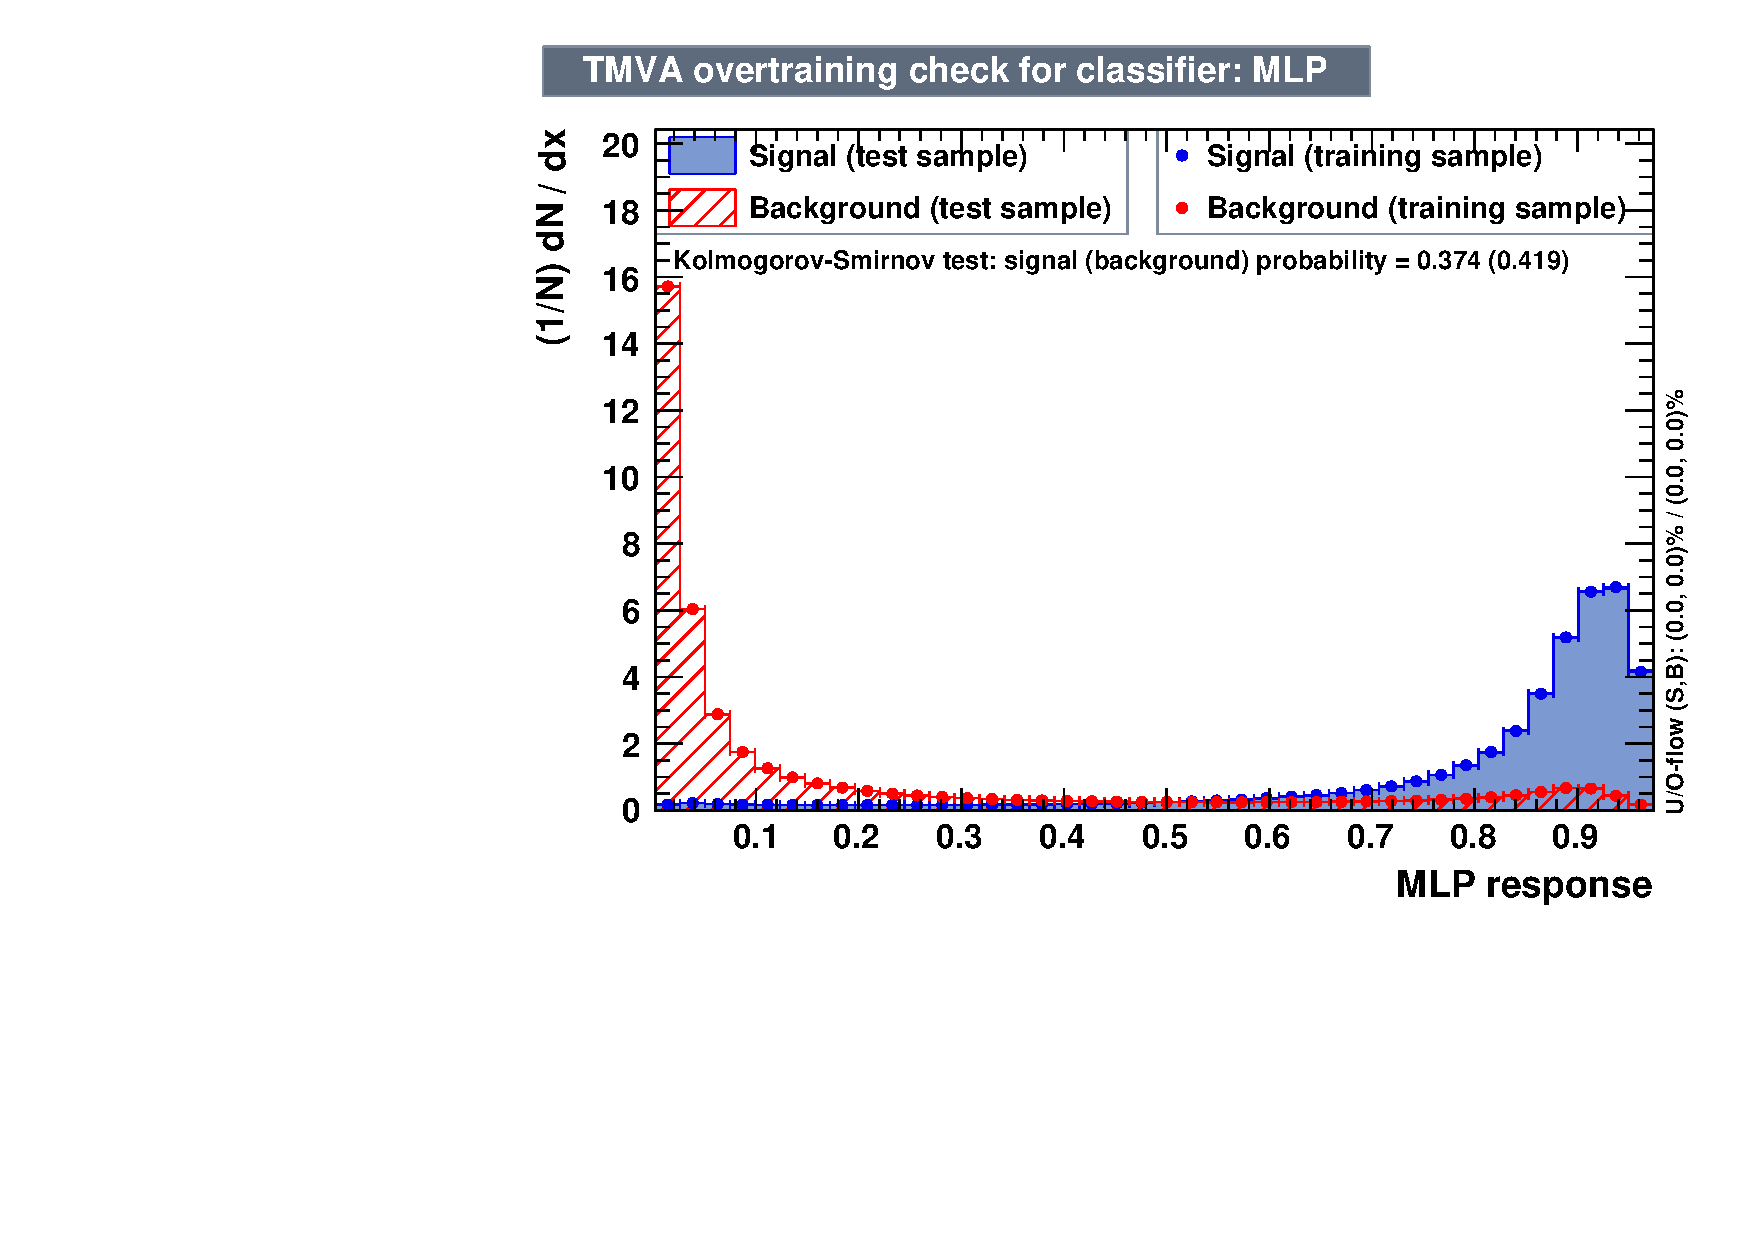
\includegraphics[width=0.4\textwidth]{Figures/EventSelReco/mva/t13_MLP_sep.pdf}}
			    \subfigure[ROC curve (8 vars)]{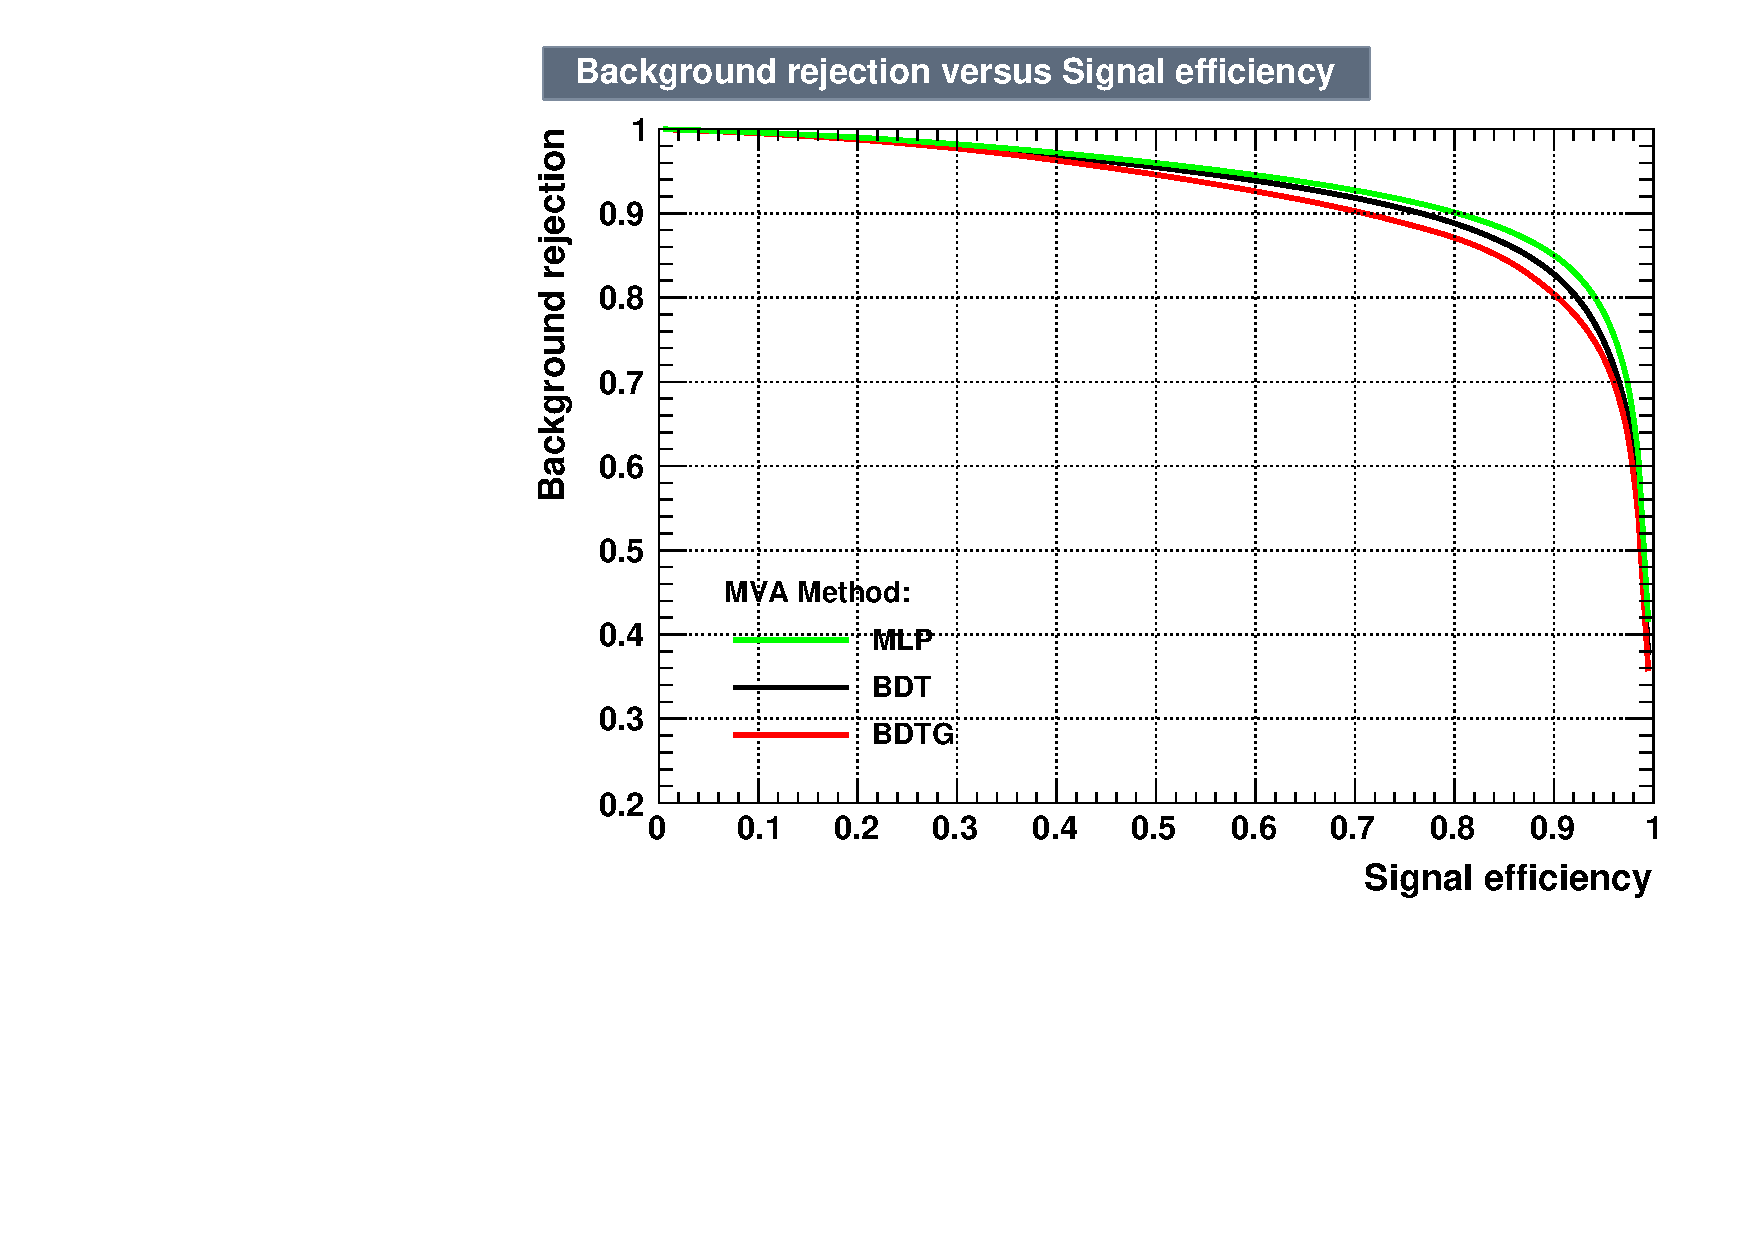
\includegraphics[width=0.4\textwidth]{Figures/EventSelReco/mva/t13_ROC.pdf}}\\
			\caption{The training result of 8 variables set}
			\label{EventSelReco:fig:Sep_ROC_t13}
			\end{figure}
			\FloatBarrier

			\begin{figure}[H]
			\centering{}
    			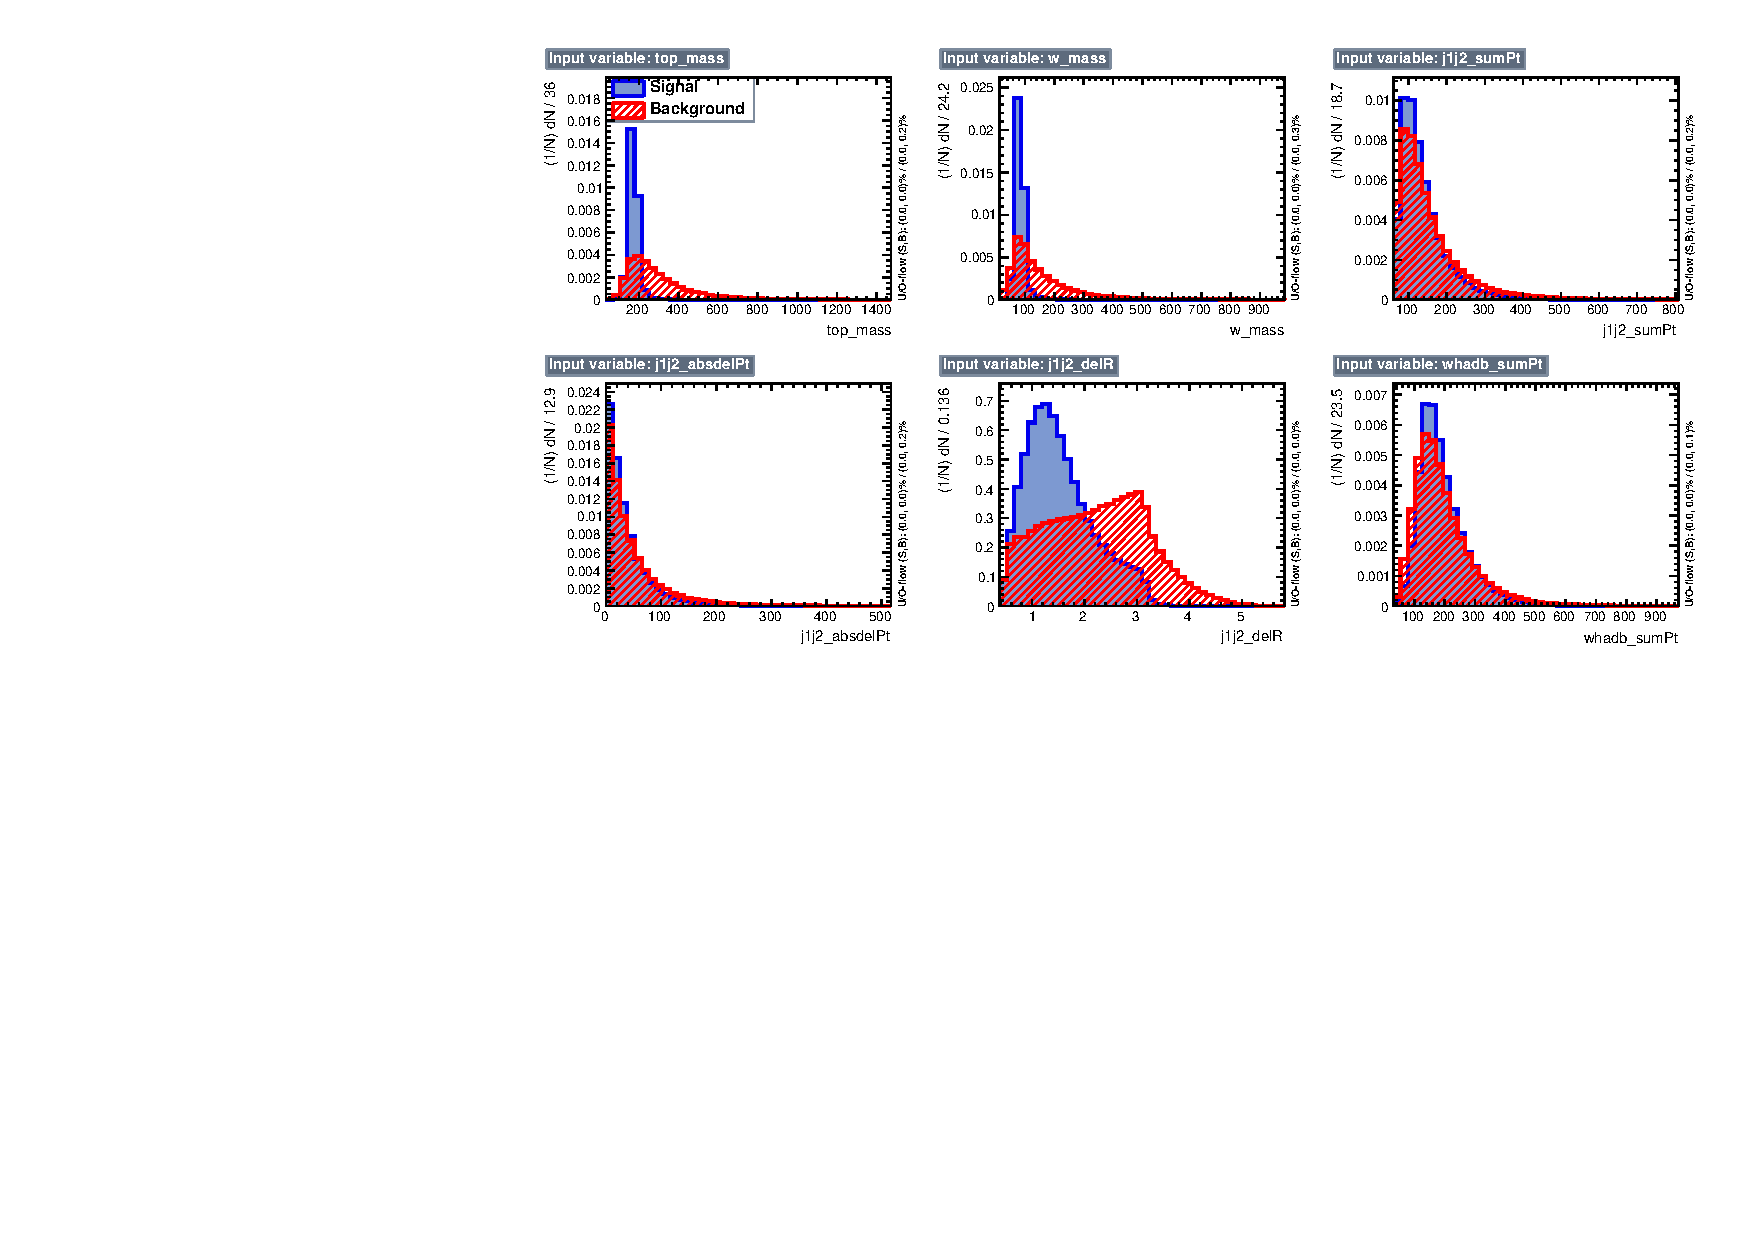
\includegraphics[width=0.8\textwidth]{Figures/EventSelReco/mva/a05_VarSep1.pdf}\\
			\end{figure}
			\FloatBarrier
			\begin{figure}[H]
			\centering{}
    			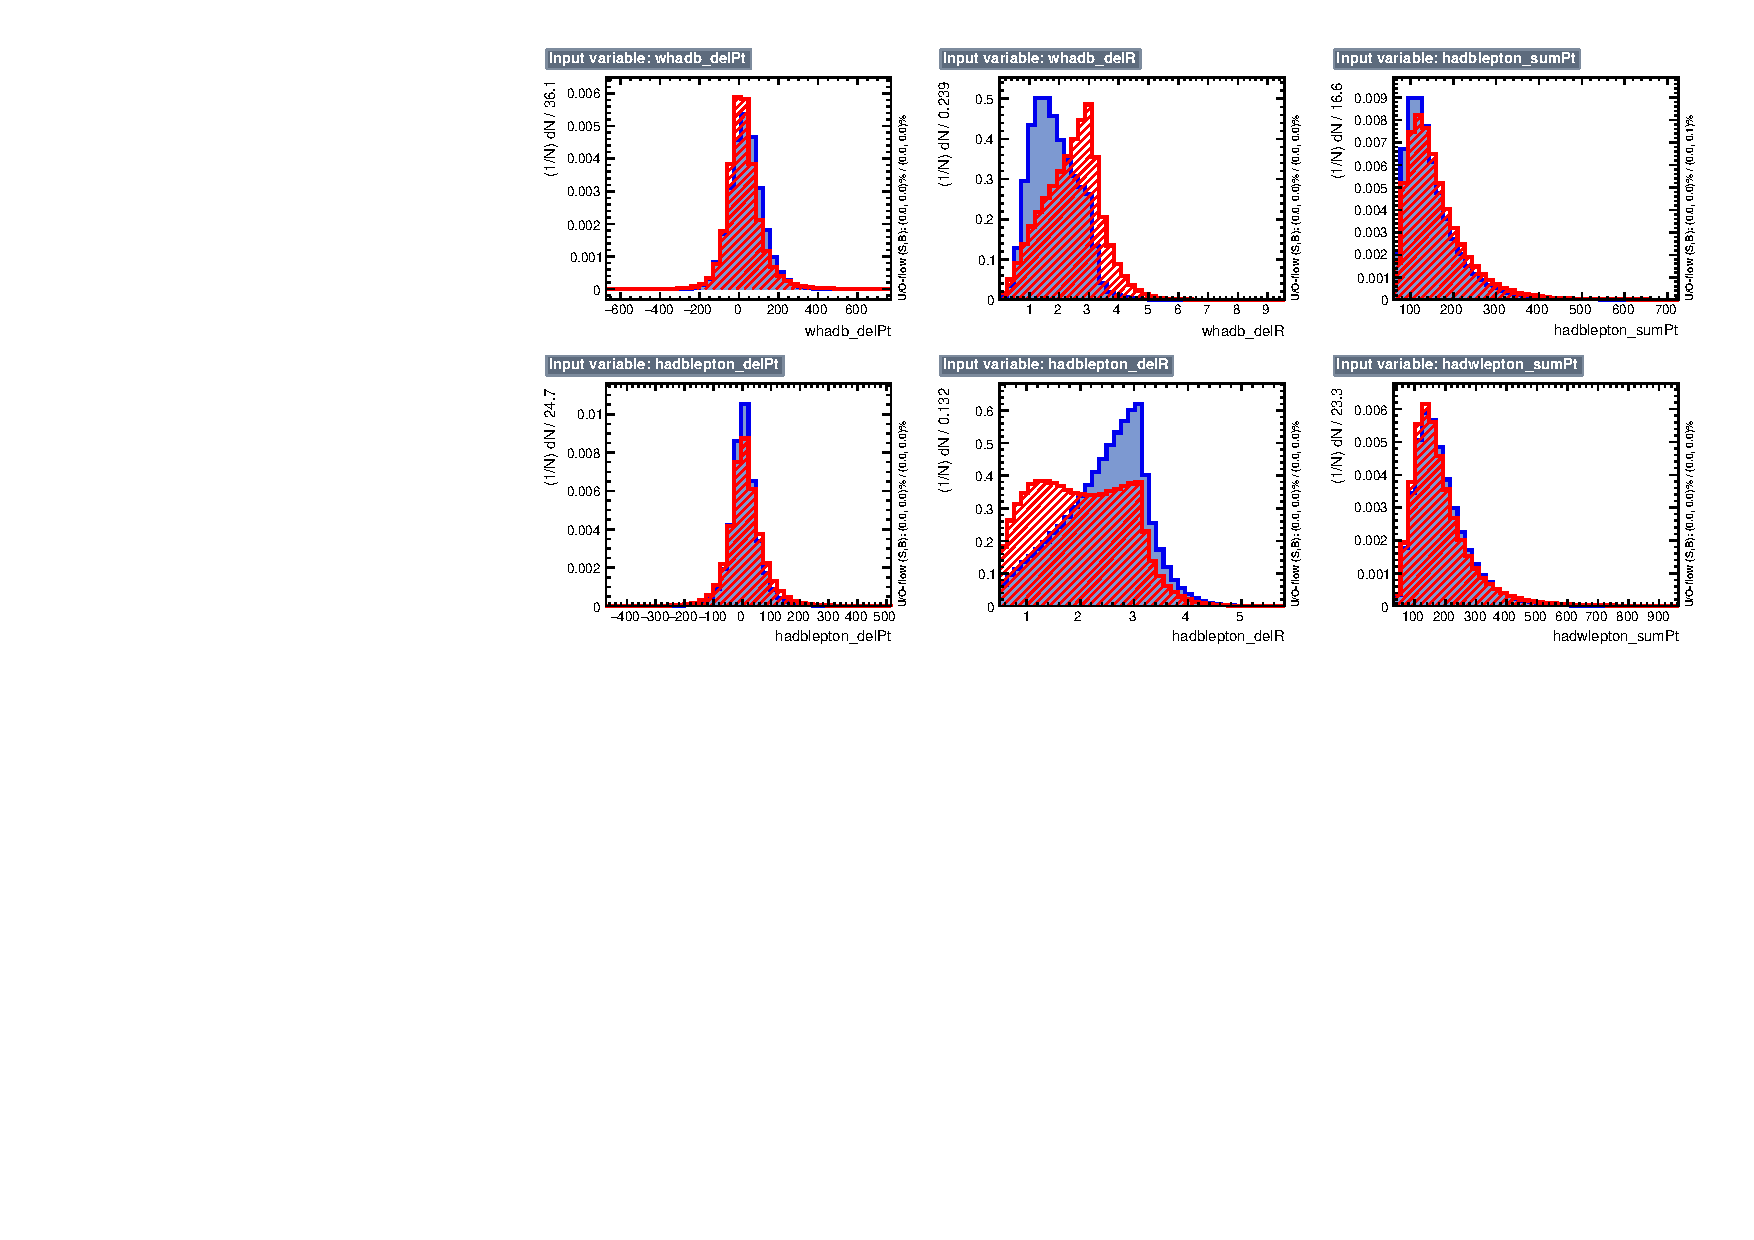
\includegraphics[width=0.8\textwidth]{Figures/EventSelReco/mva/a05_VarSep2.pdf}\\
			\end{figure}
			\FloatBarrier
			\begin{figure}[H]
			\centering{}
    			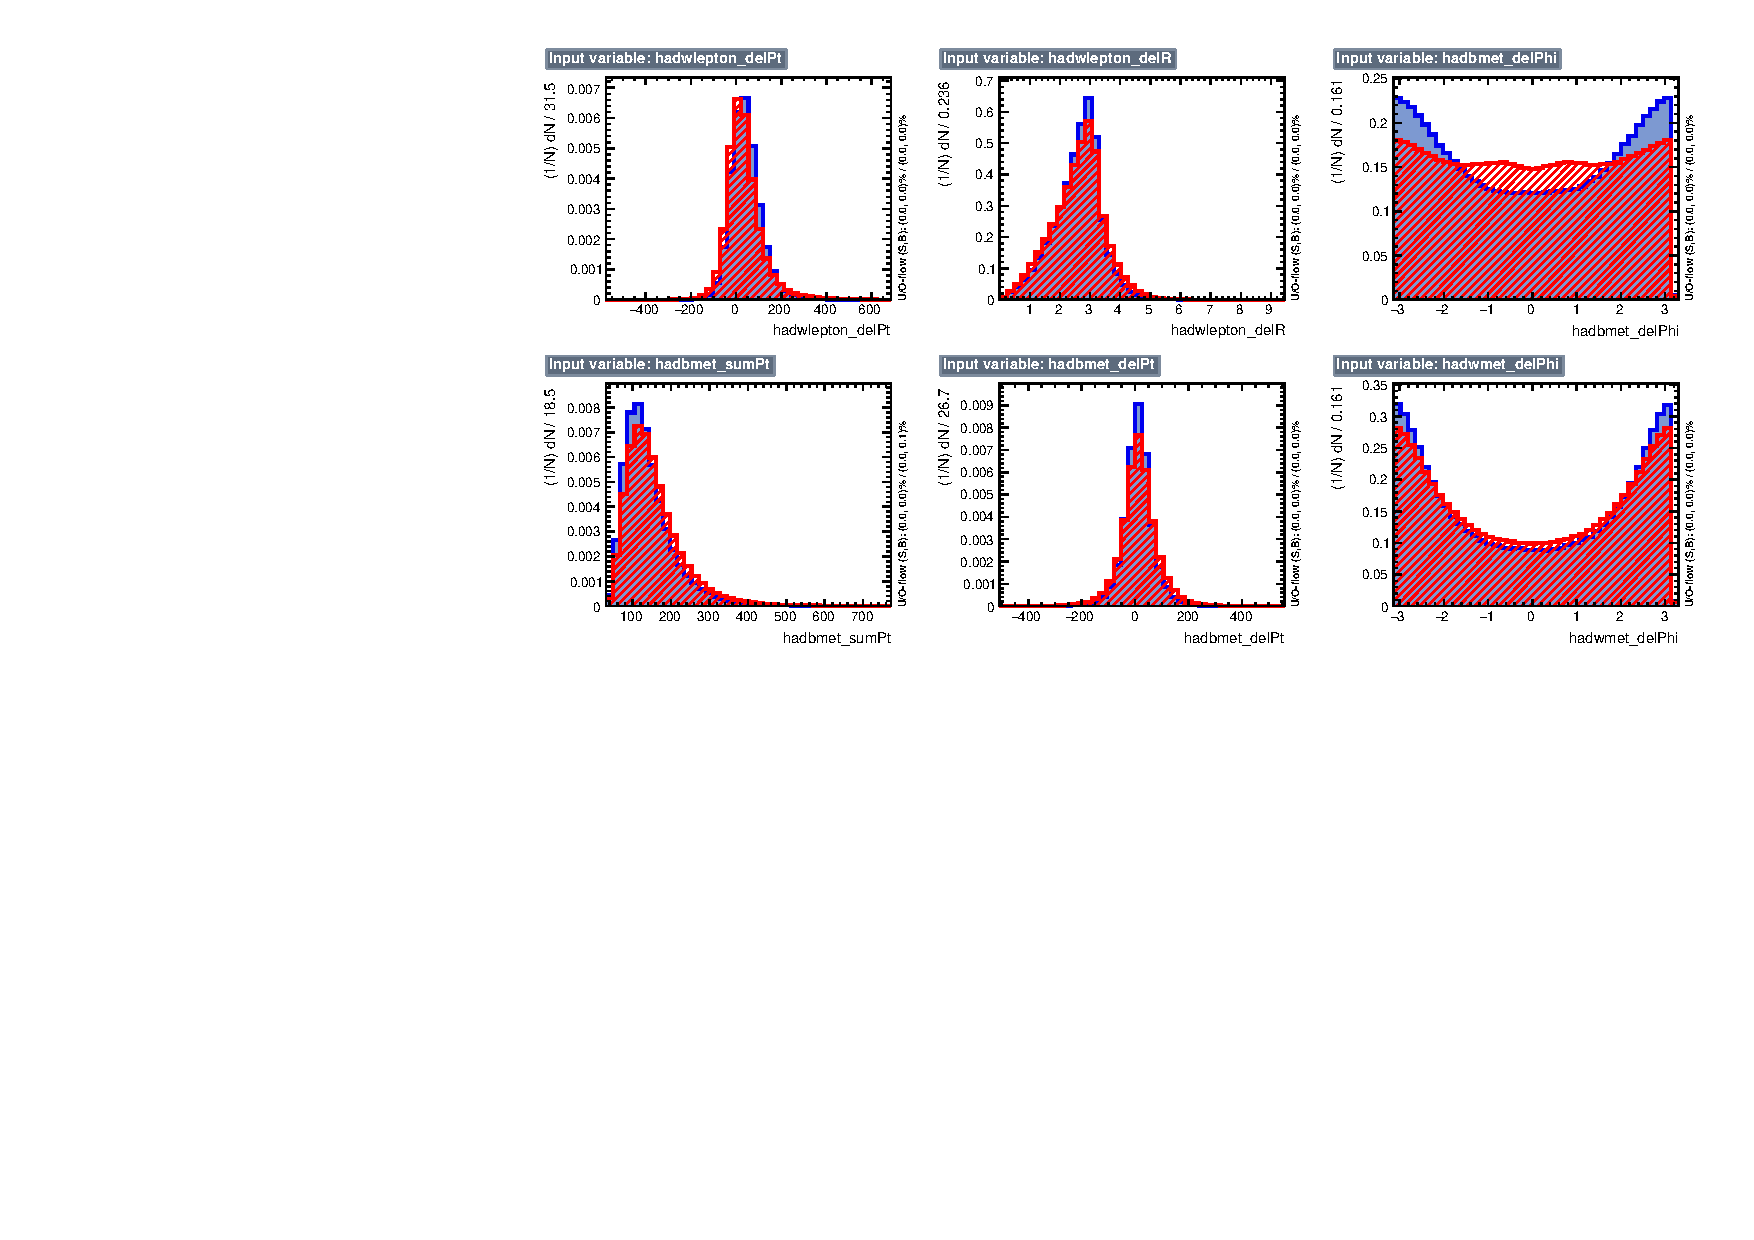
\includegraphics[width=0.8\textwidth]{Figures/EventSelReco/mva/a05_VarSep3.pdf}\\
			\end{figure}
			\FloatBarrier
			\begin{figure}[H]
			\centering{}
    			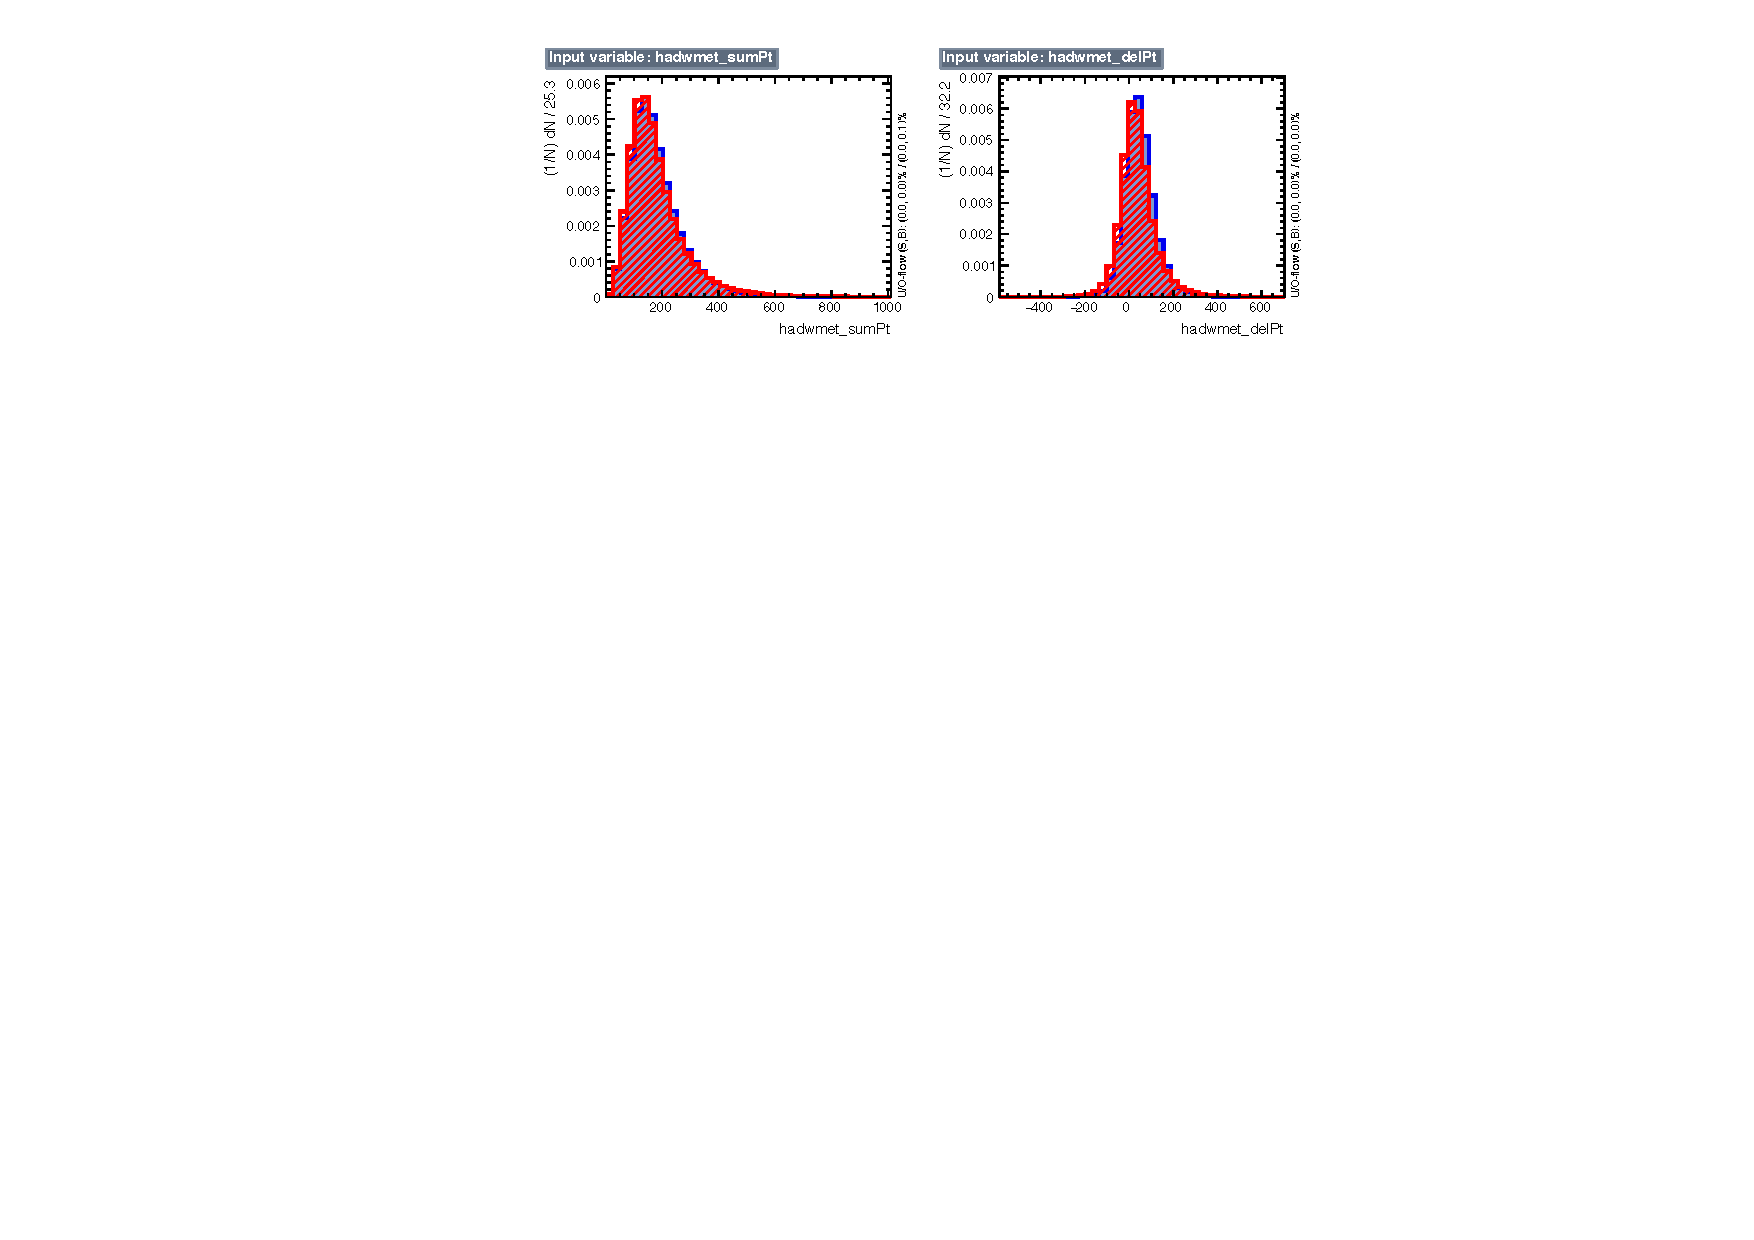
\includegraphics[width=0.528\textwidth]{Figures/EventSelReco/mva/a05_VarSep4.pdf}\\
    		\caption{Input training variables separation between $"$signal$"$ and $"$background$"$.(20 variables)}
			\label{EventSelReco:fig:a05_varsep}
			\end{figure}
			\FloatBarrier


			\begin{figure}[H]
			\centering
				\subfigure[BDT's separation result (20 vars)]{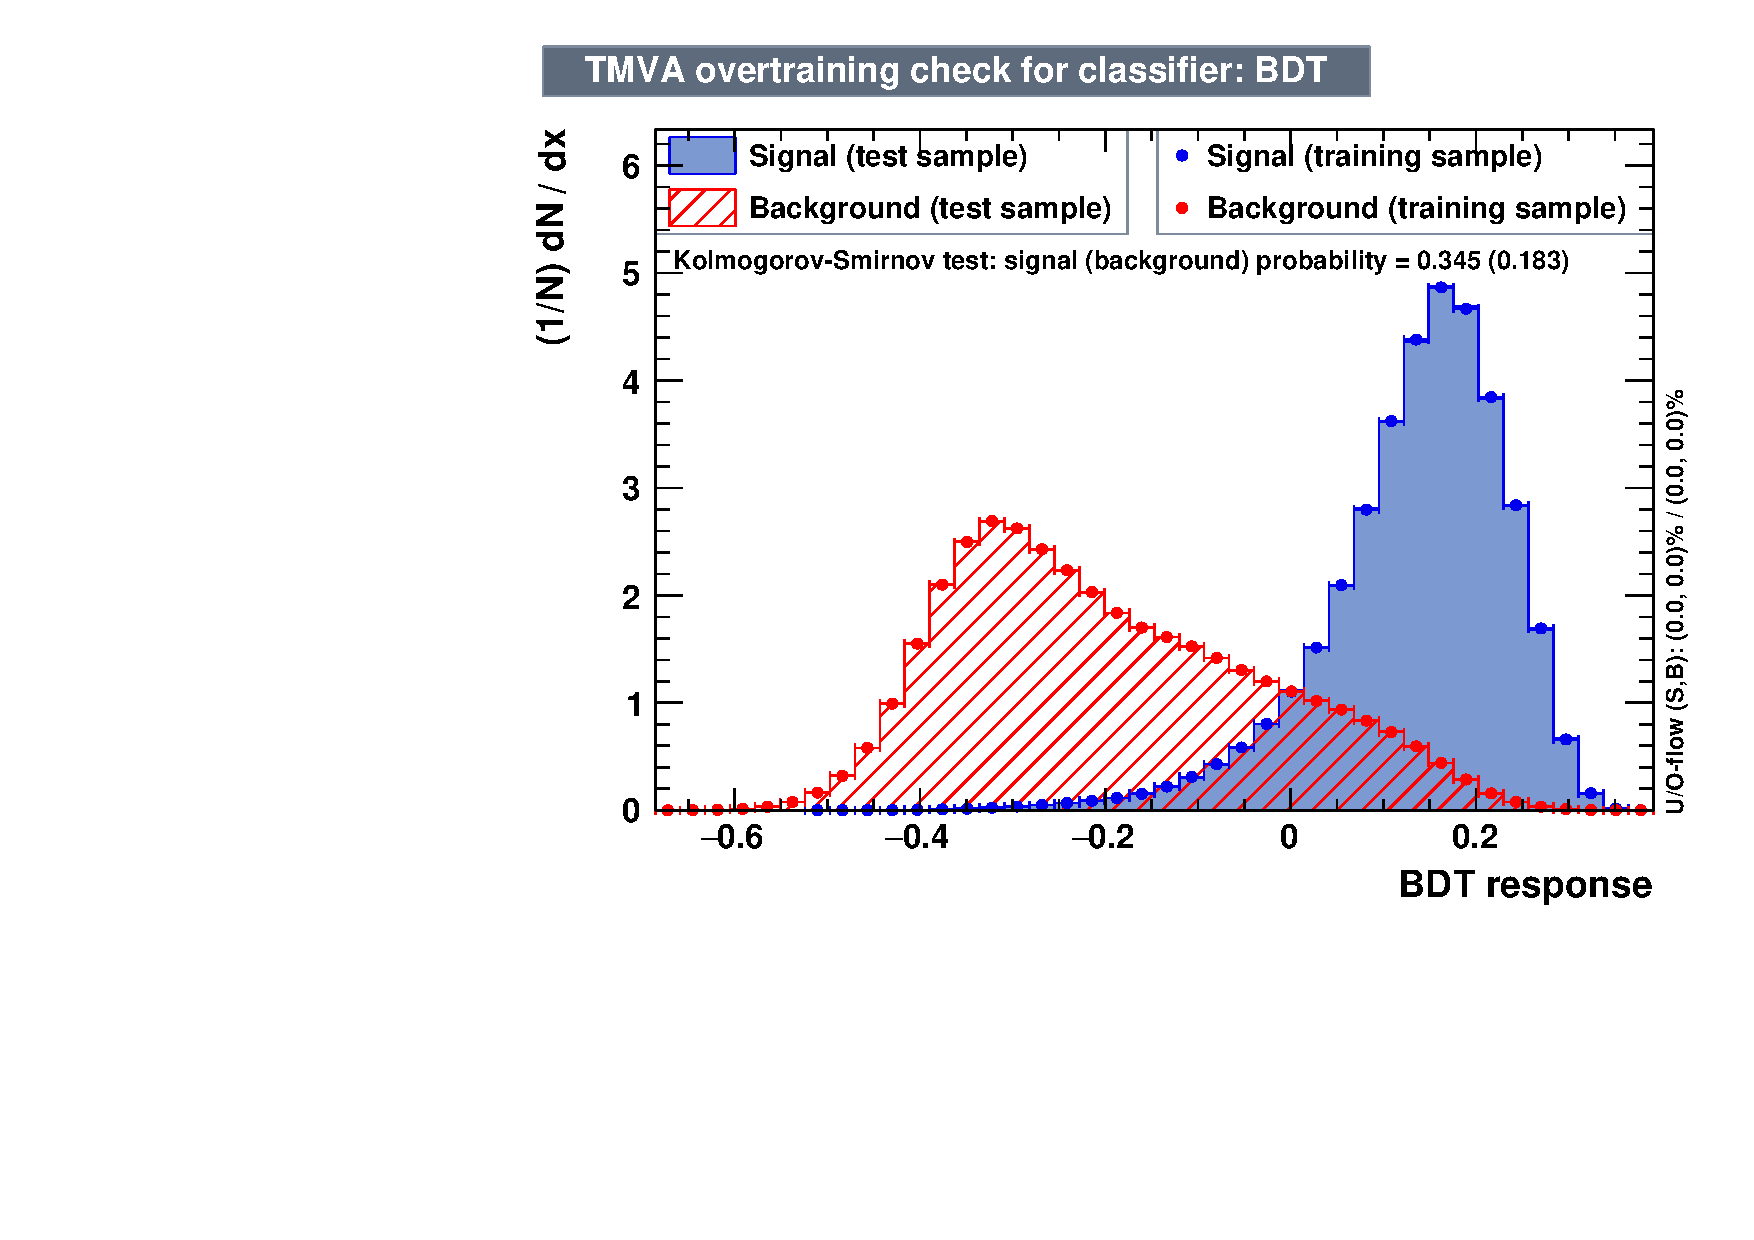
\includegraphics[width=0.4\textwidth]{Figures/EventSelReco/mva/a05_all_BDT_sep.pdf}}
			    \subfigure[BDTG's separation result (20 vars)]{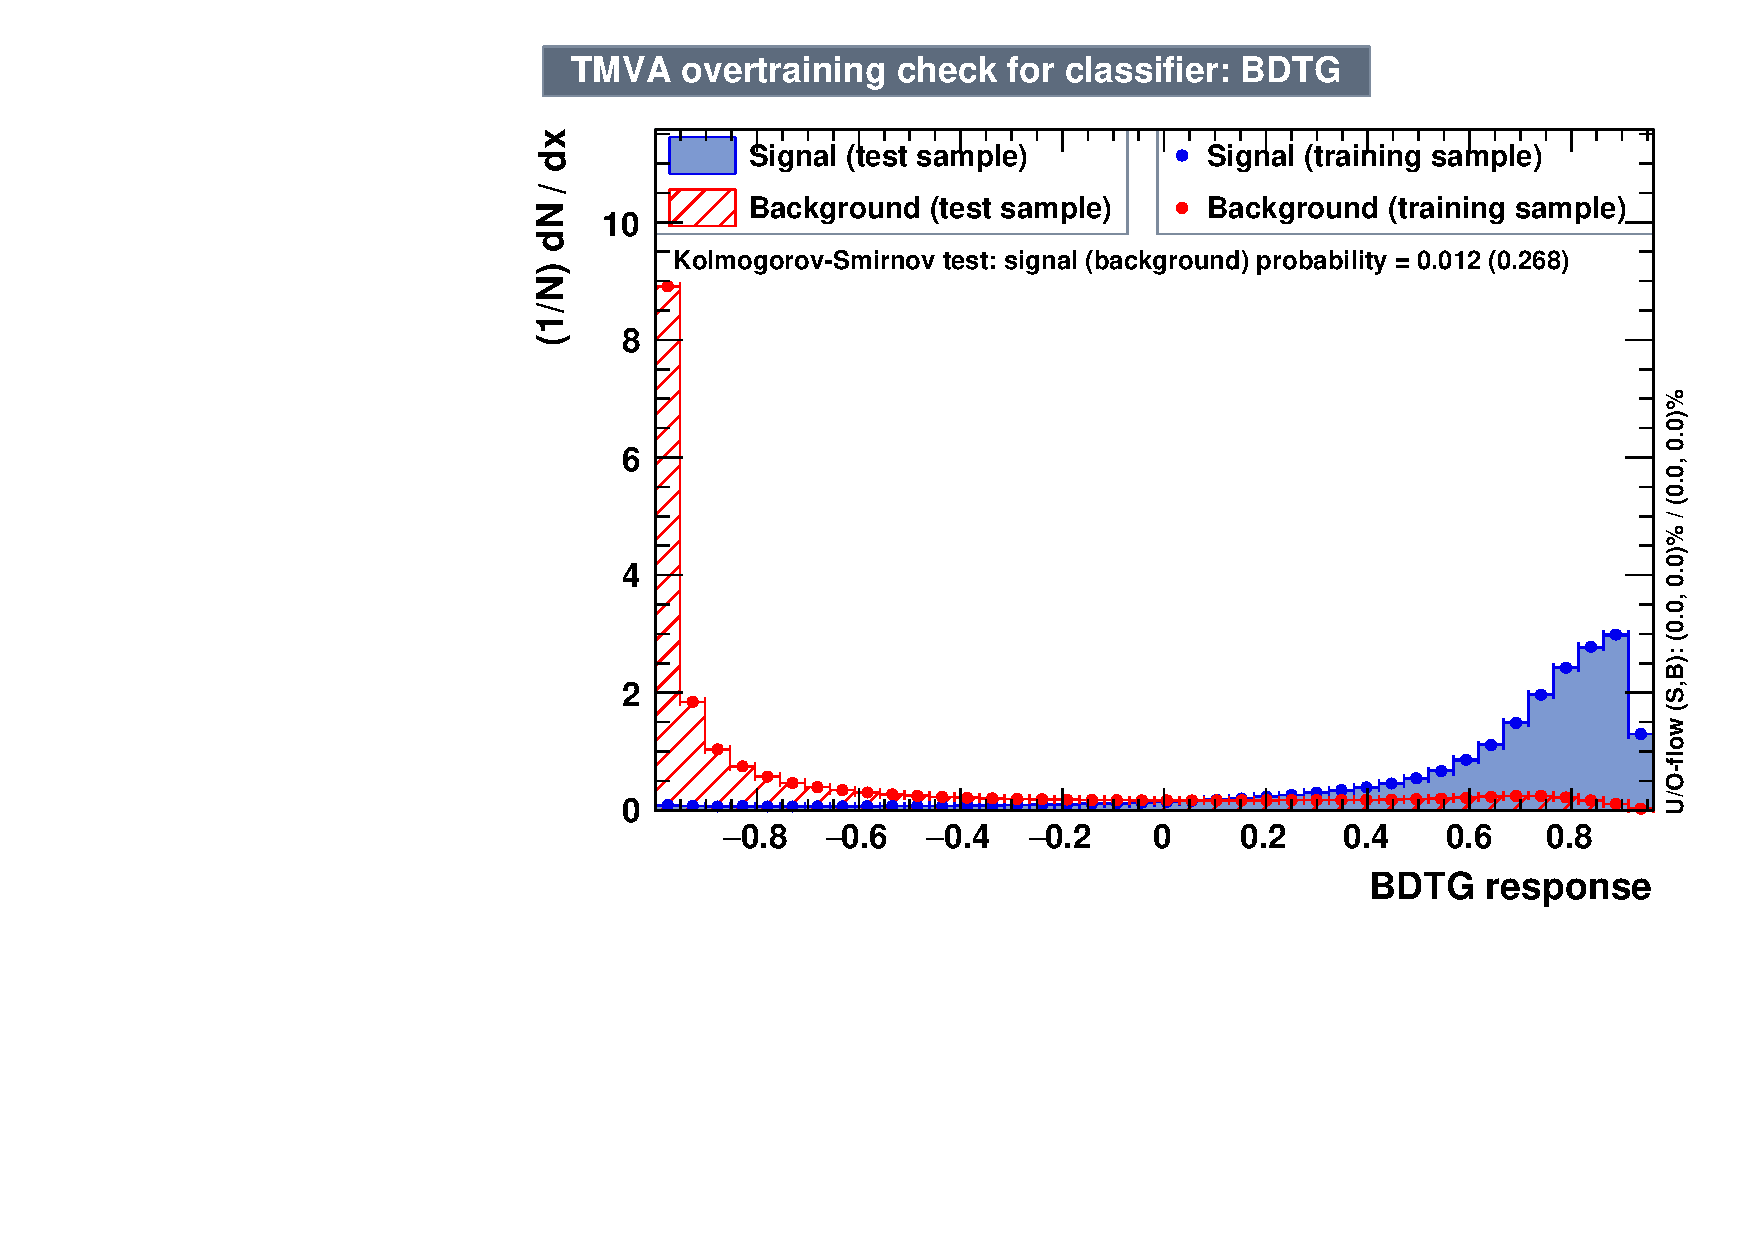
\includegraphics[width=0.4\textwidth]{Figures/EventSelReco/mva/a05_all_BDTG_sep.pdf}}\\
			\end{figure}
			\FloatBarrier
			\begin{figure}[H]
			\centering
			    \subfigure[MLP's separation result (20 vars)]{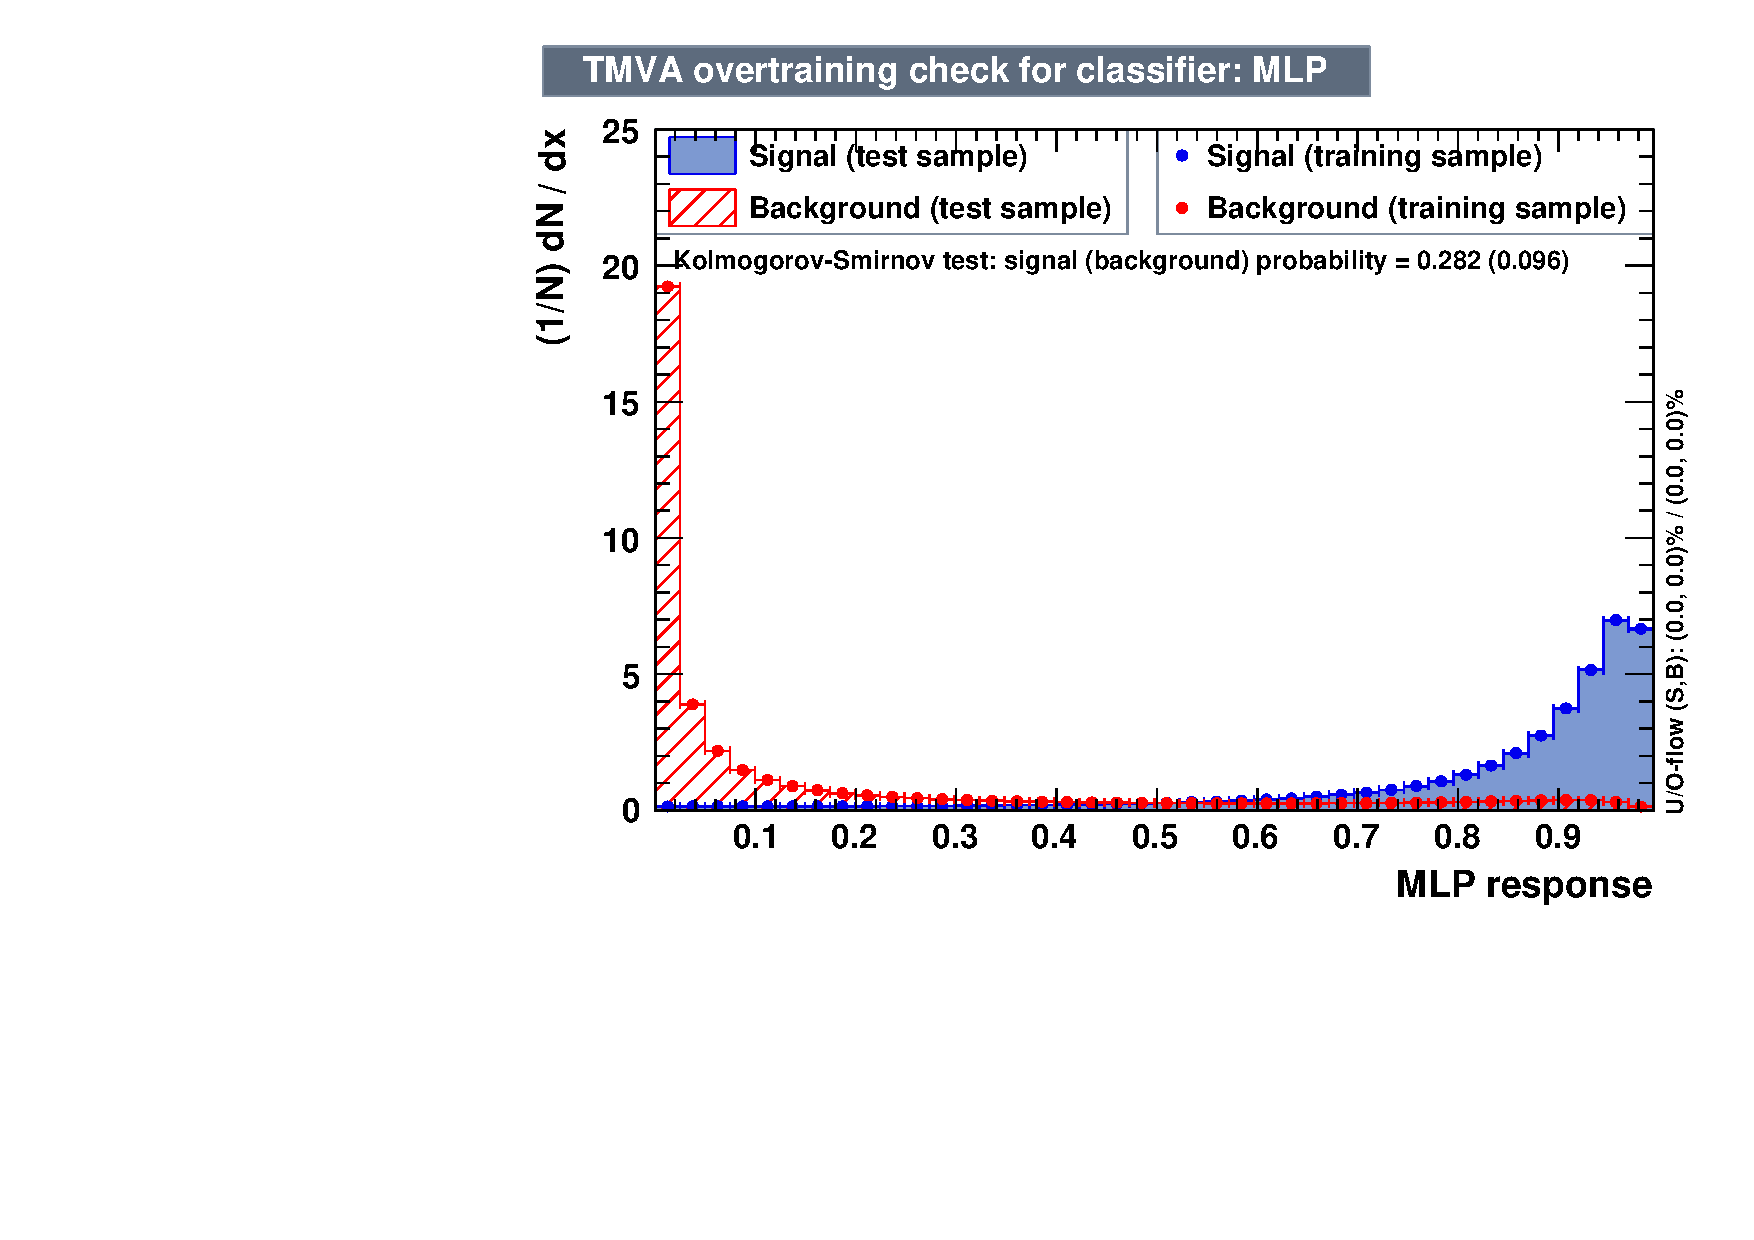
\includegraphics[width=0.4\textwidth]{Figures/EventSelReco/mva/a05_all_MLP_sep.pdf}}
			    \subfigure[ROC curve (20 vars)]{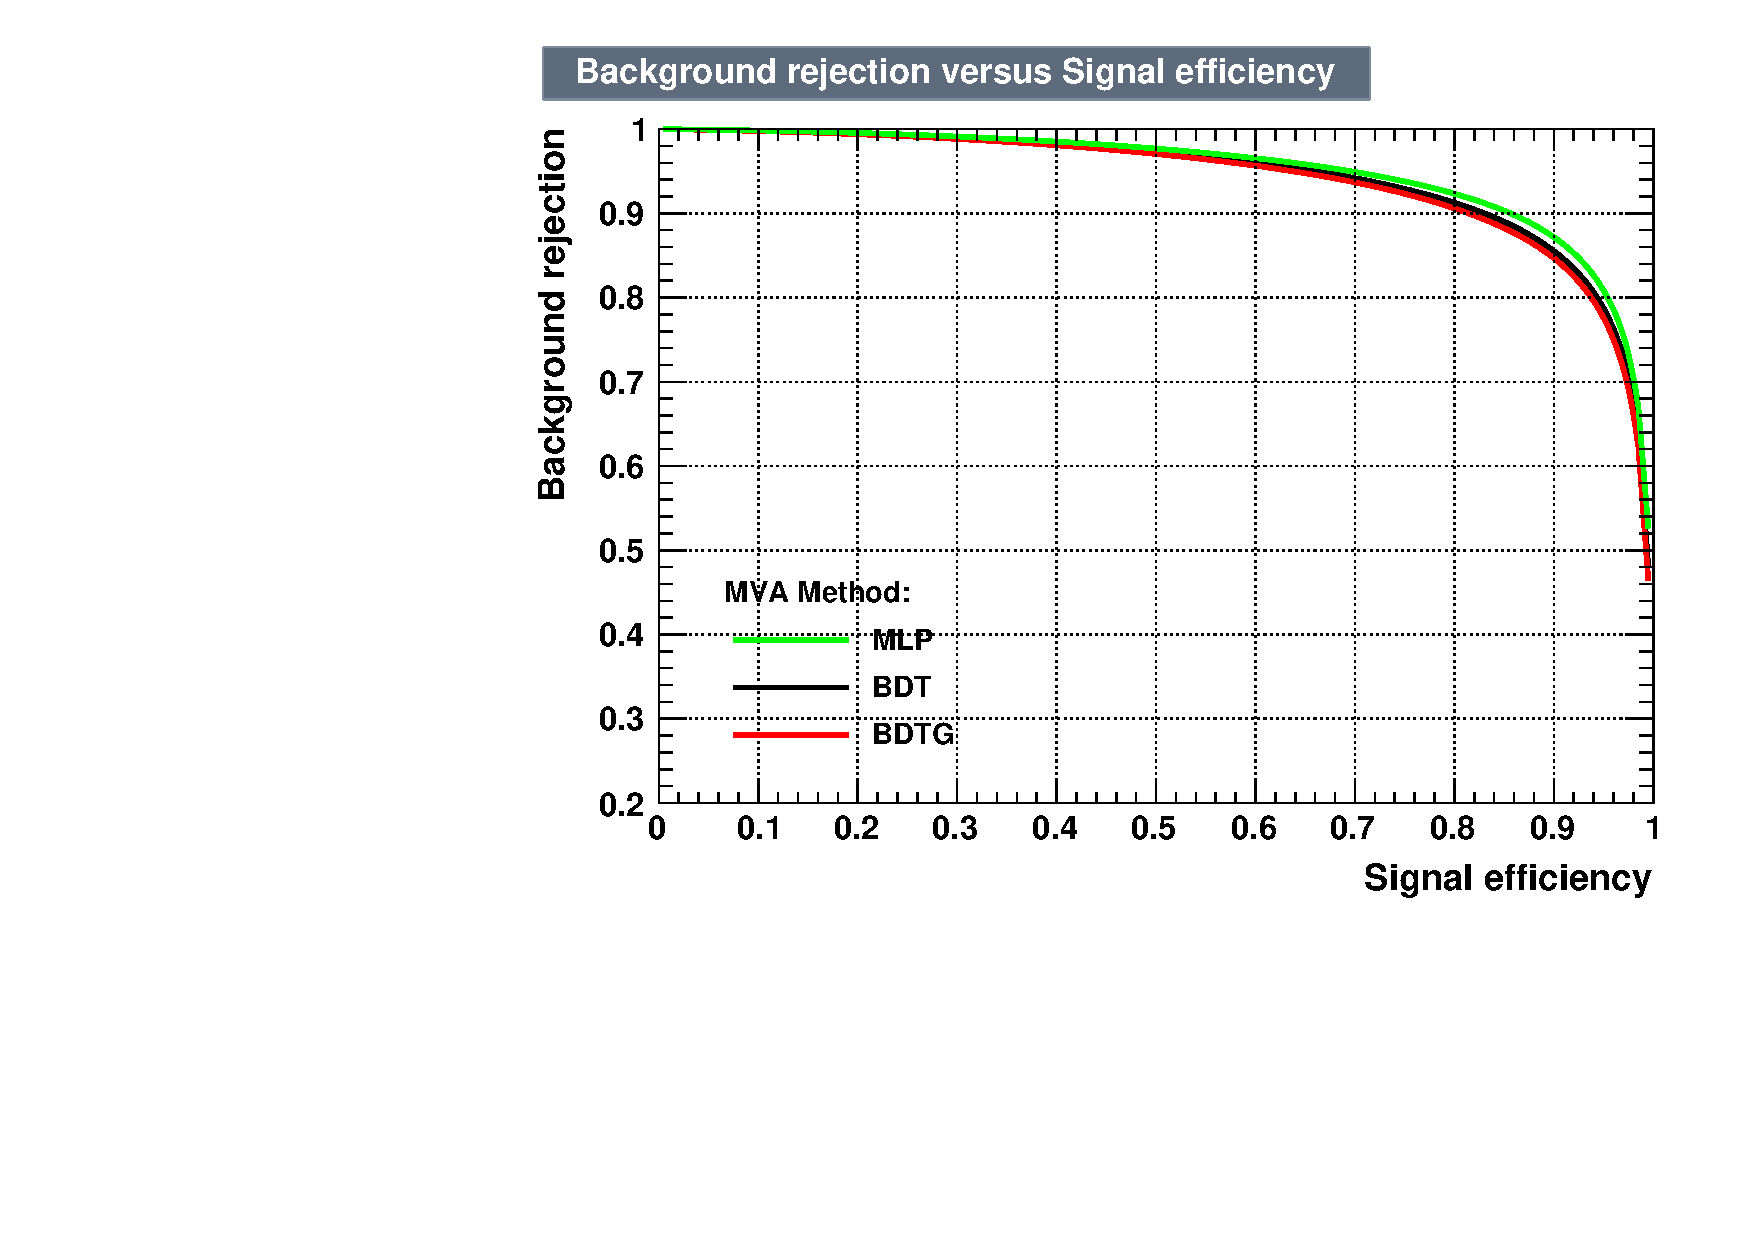
\includegraphics[width=0.4\textwidth]{Figures/EventSelReco/mva/a05_all_ROC.pdf}}\\
			\caption{The training result of 20 variables set}
			\label{EventSelReco:fig:Sep_ROC_a05}
			\end{figure}
			\FloatBarrier

			This is shown that the MLP(ANN) training algorithm has the best performance under ROC criteria from training results. But as previous mentioning, the ROC performance cannot totally represent the training performance completely in these analysis case.

			There are results of reconstructed $M_{jjb}$ by 8 variables' and 20 variables' MLP algorithm.

			\begin{figure}[H]
			\centering
				\subfigure[muon channel]{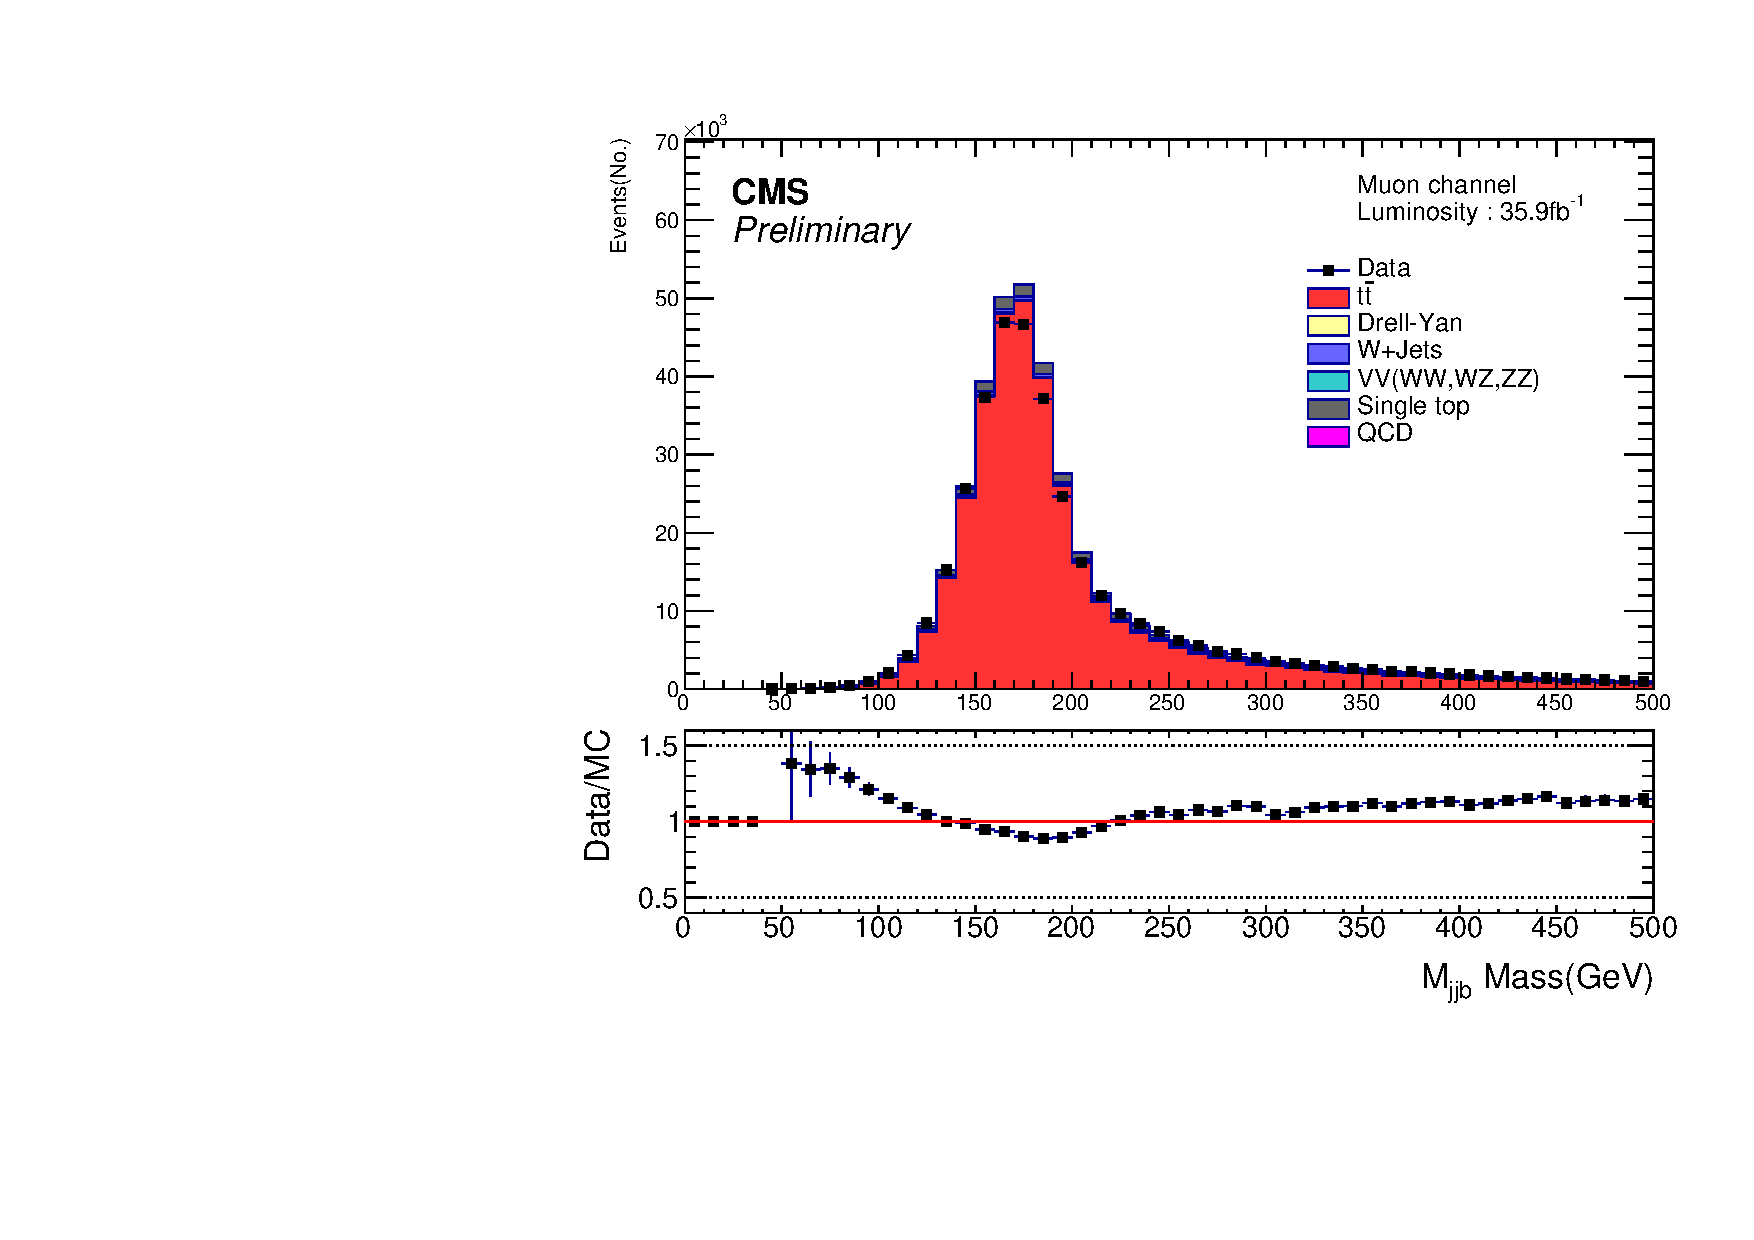
\includegraphics[width=0.45\textwidth]{Figures/EventSelReco/Mass/t13/t13_MLP_NC_long_HadTop_mu.pdf}}
			    \subfigure[electron channel]{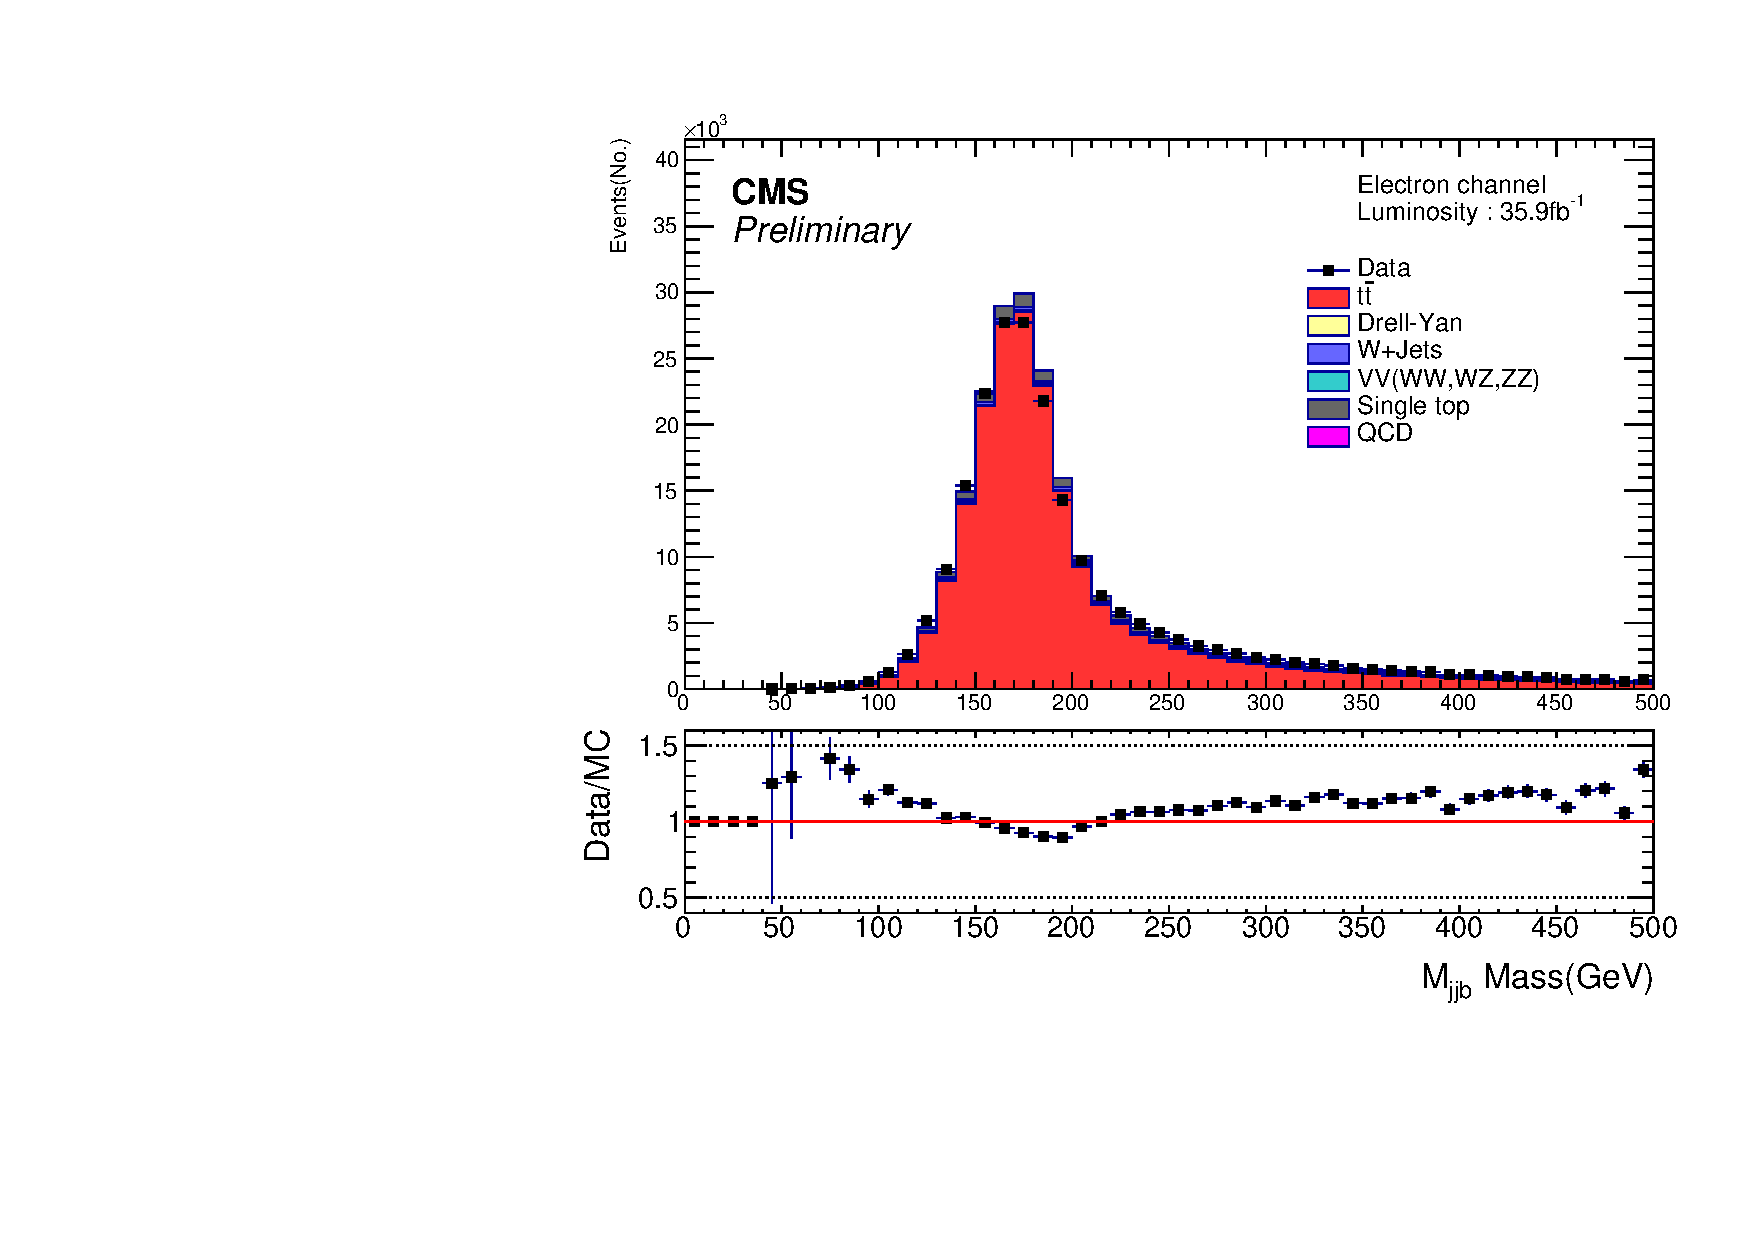
\includegraphics[width=0.45\textwidth]{Figures/EventSelReco/Mass/t13/t13_MLP_NC_long_HadTop_el.pdf}}\\
			\caption{Reconstructed $M_{jjb}$ with 8 variables MLP algorithm (w/o cut)}
			\label{EventSelReco:fig:t13_MLP_SR_NC_Mjjb}
			\end{figure}
			\FloatBarrier

			\begin{figure}[H]
			\centering
				\subfigure[muon channel]{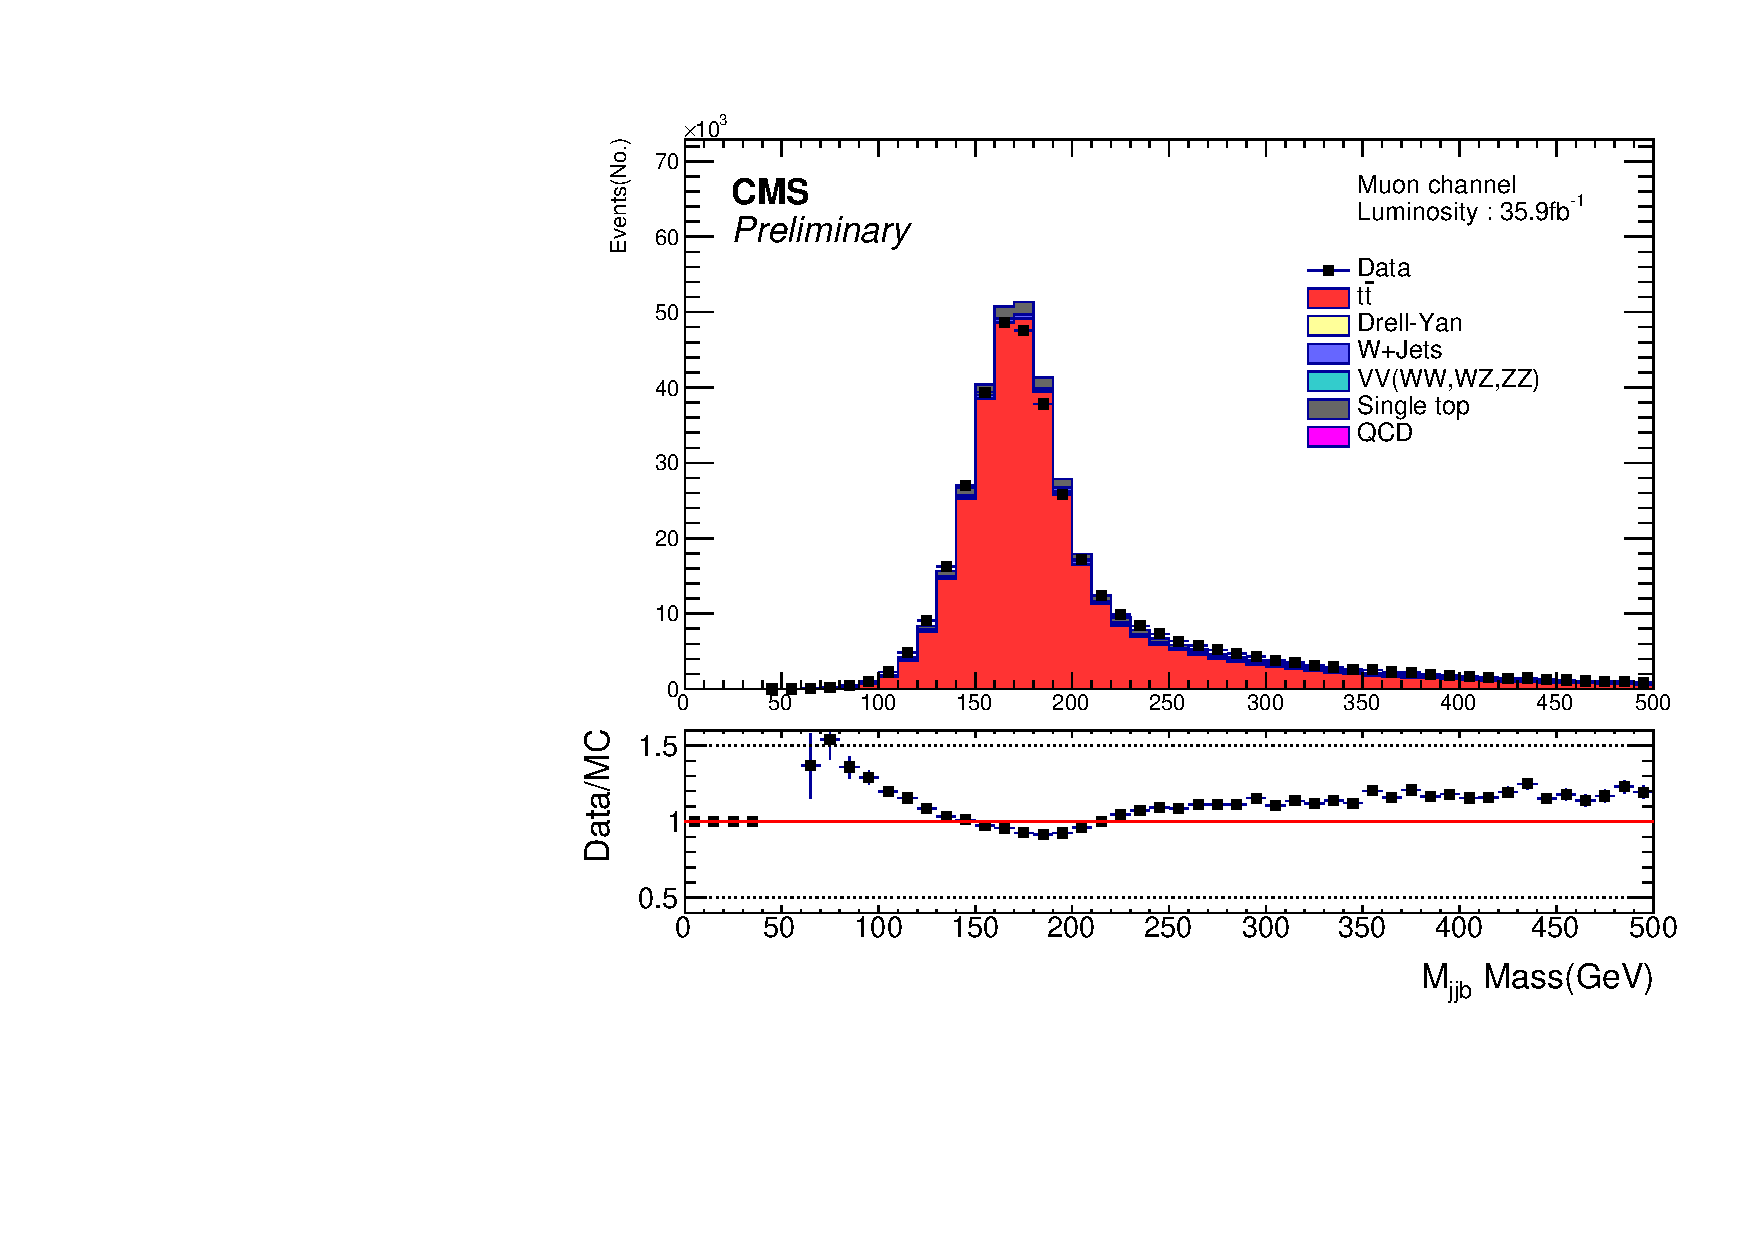
\includegraphics[width=0.45\textwidth]{Figures/EventSelReco/Mass/a05/a05_MLP_NC_long_HadTop_mu.pdf}}
			    \subfigure[electron channel]{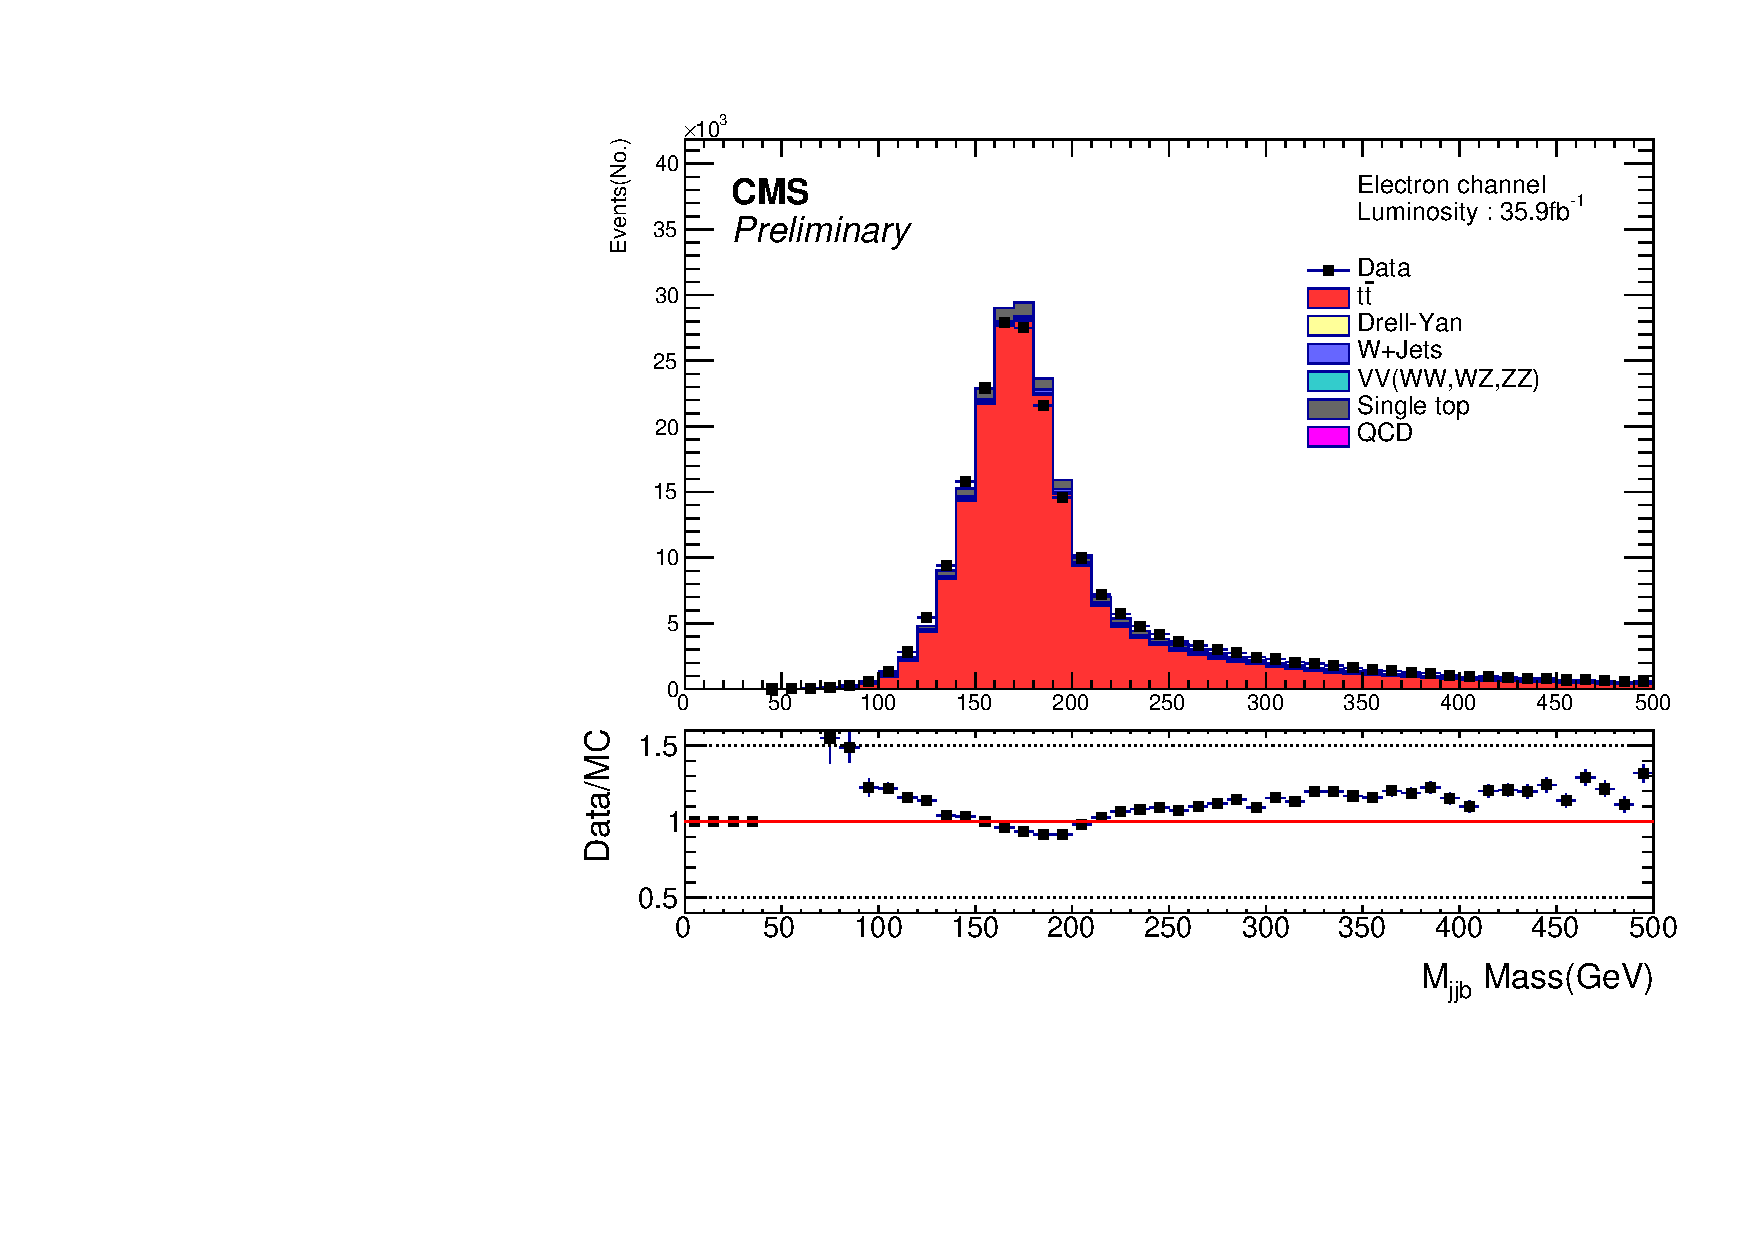
\includegraphics[width=0.45\textwidth]{Figures/EventSelReco/Mass/a05/a05_MLP_NC_long_HadTop_el.pdf}}\\
			\caption{Reconstructed $M_{jjb}$ with 20 variables MLP algorithm (w/o cut)}
			\label{EventSelReco:fig:a05_MLP_SR_NC_Mjjb}
			\end{figure}
			\FloatBarrier

			There are the max MVA score's distribution with 2/8/20 variables and BDT/BDTG/MLP results.

			\begin{figure}[H]
			\centering
				\subfigure[BDT (2 vars, mu-ch)]{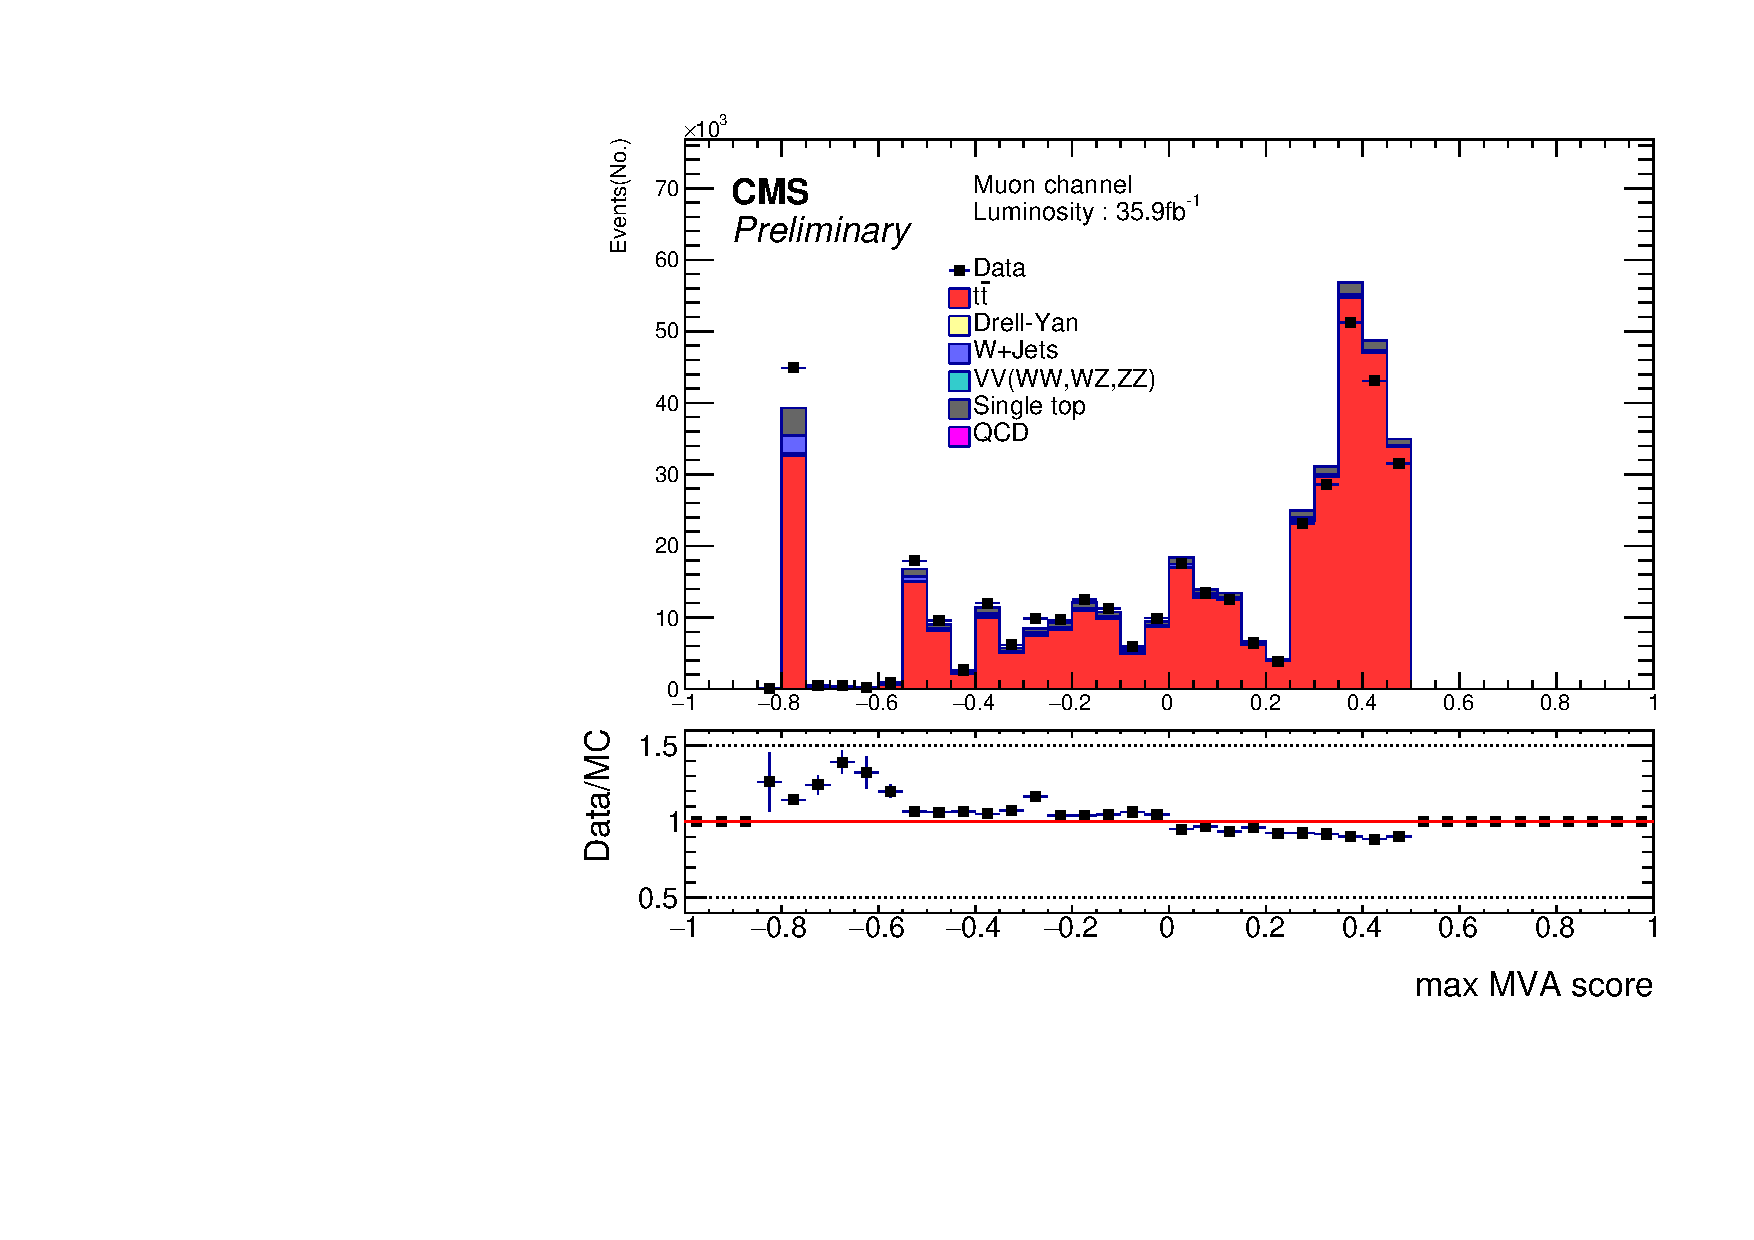
\includegraphics[width=0.32\textwidth]{Figures/EventSelReco/mva_algo/a04_BDT_SR_algo_mu.pdf}}
			    \subfigure[BDTG (2 vars, mu-ch)]{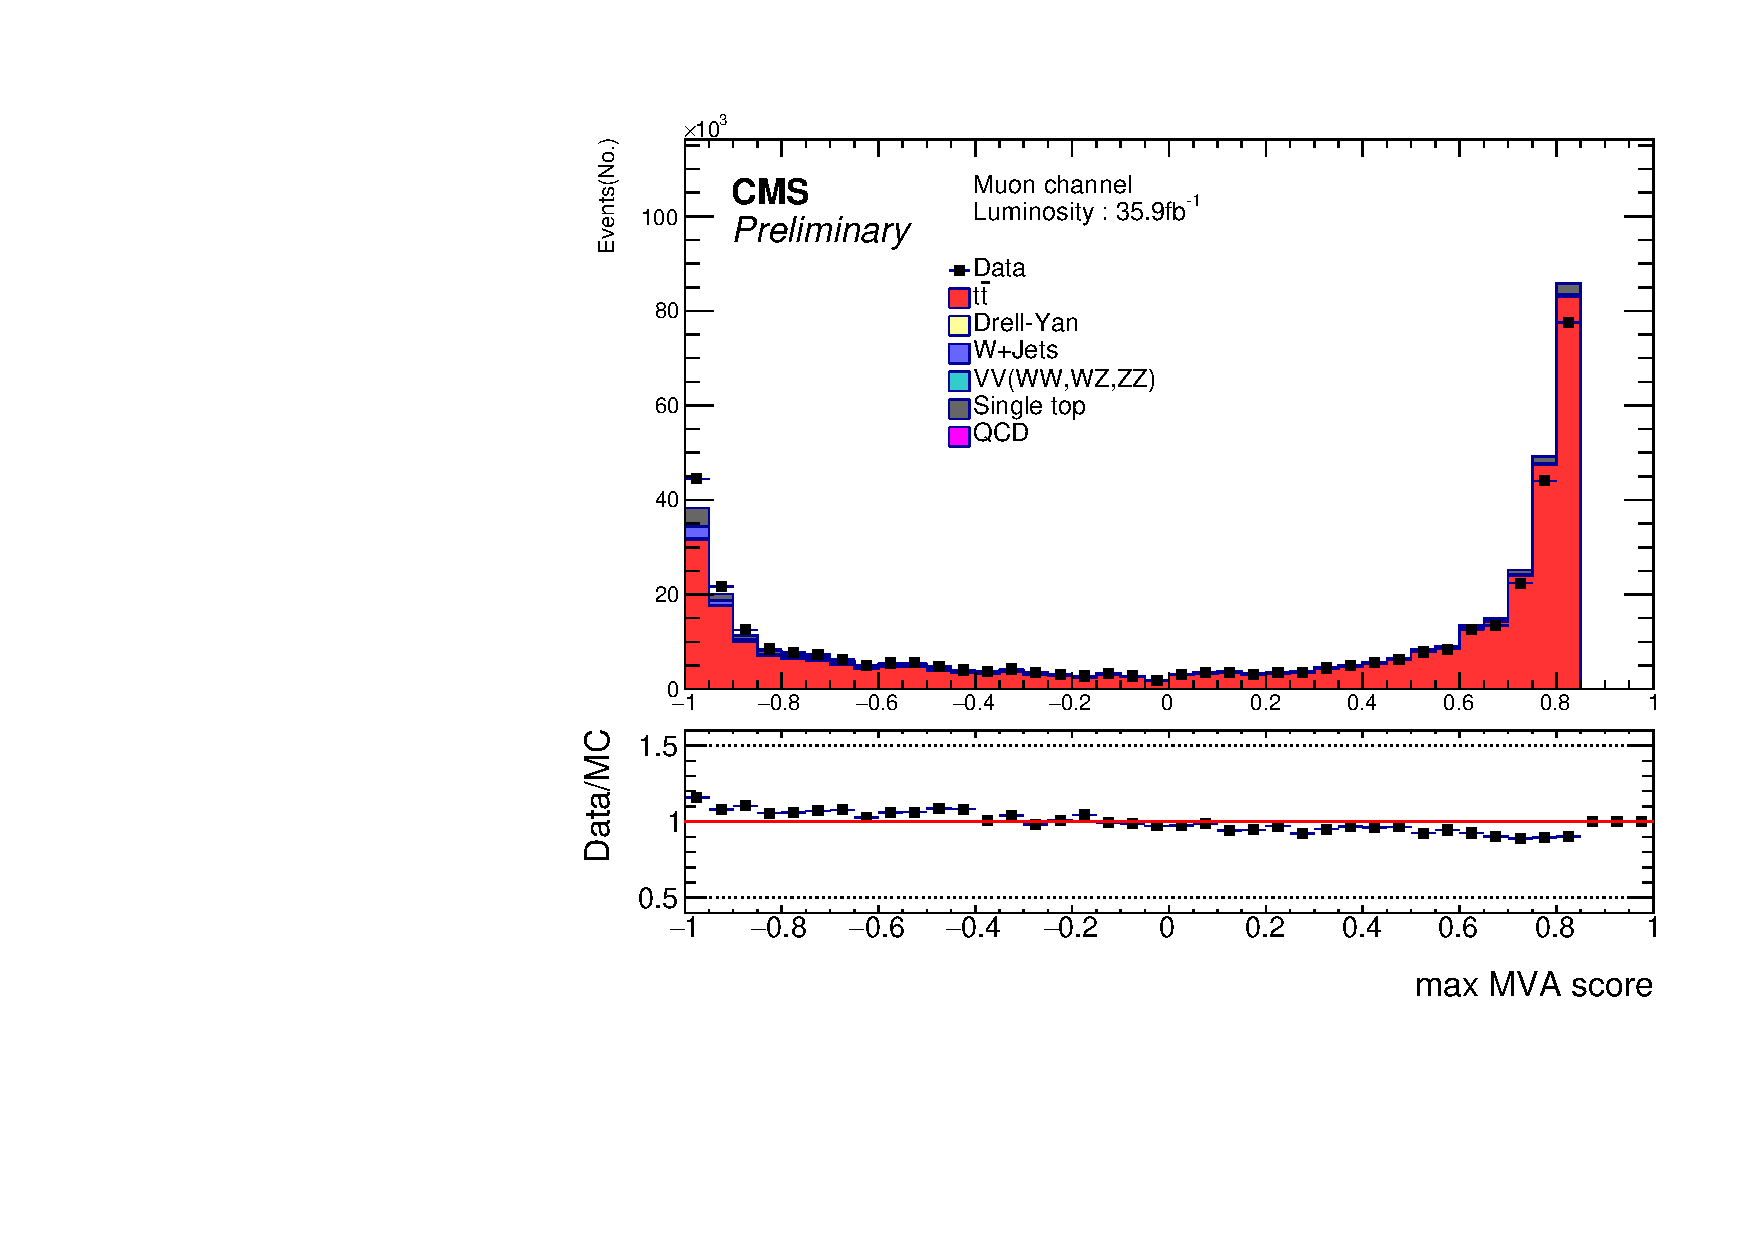
\includegraphics[width=0.32\textwidth]{Figures/EventSelReco/mva_algo/a04_BDTG_SR_algo_mu.pdf}}
			    \subfigure[MLP (2 vars, mu-ch)]{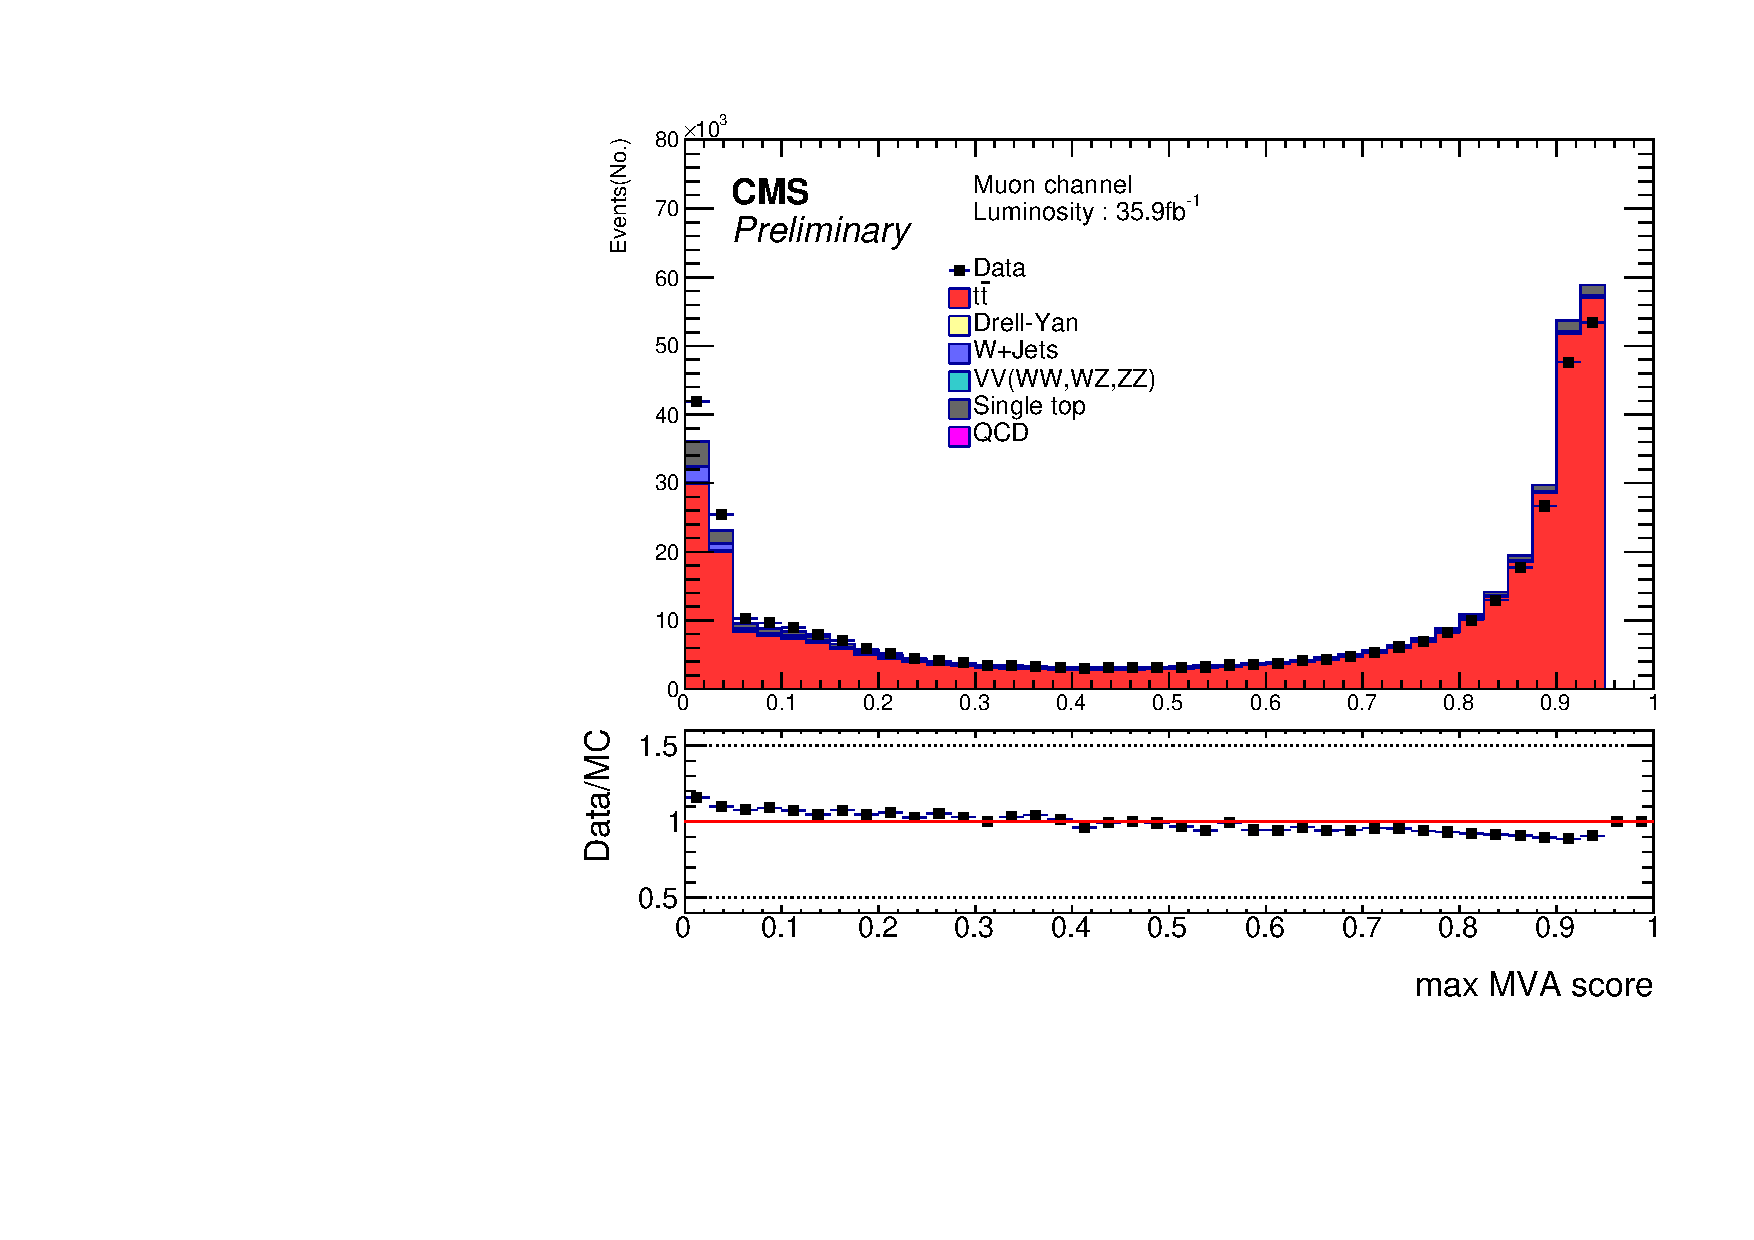
\includegraphics[width=0.32\textwidth]{Figures/EventSelReco/mva_algo/a04_MLP_SR_algo_mu.pdf}}\\
			\end{figure}
			\FloatBarrier
			\begin{figure}[H]
			\centering
			    \subfigure[BDT (2 vars, el-ch)]{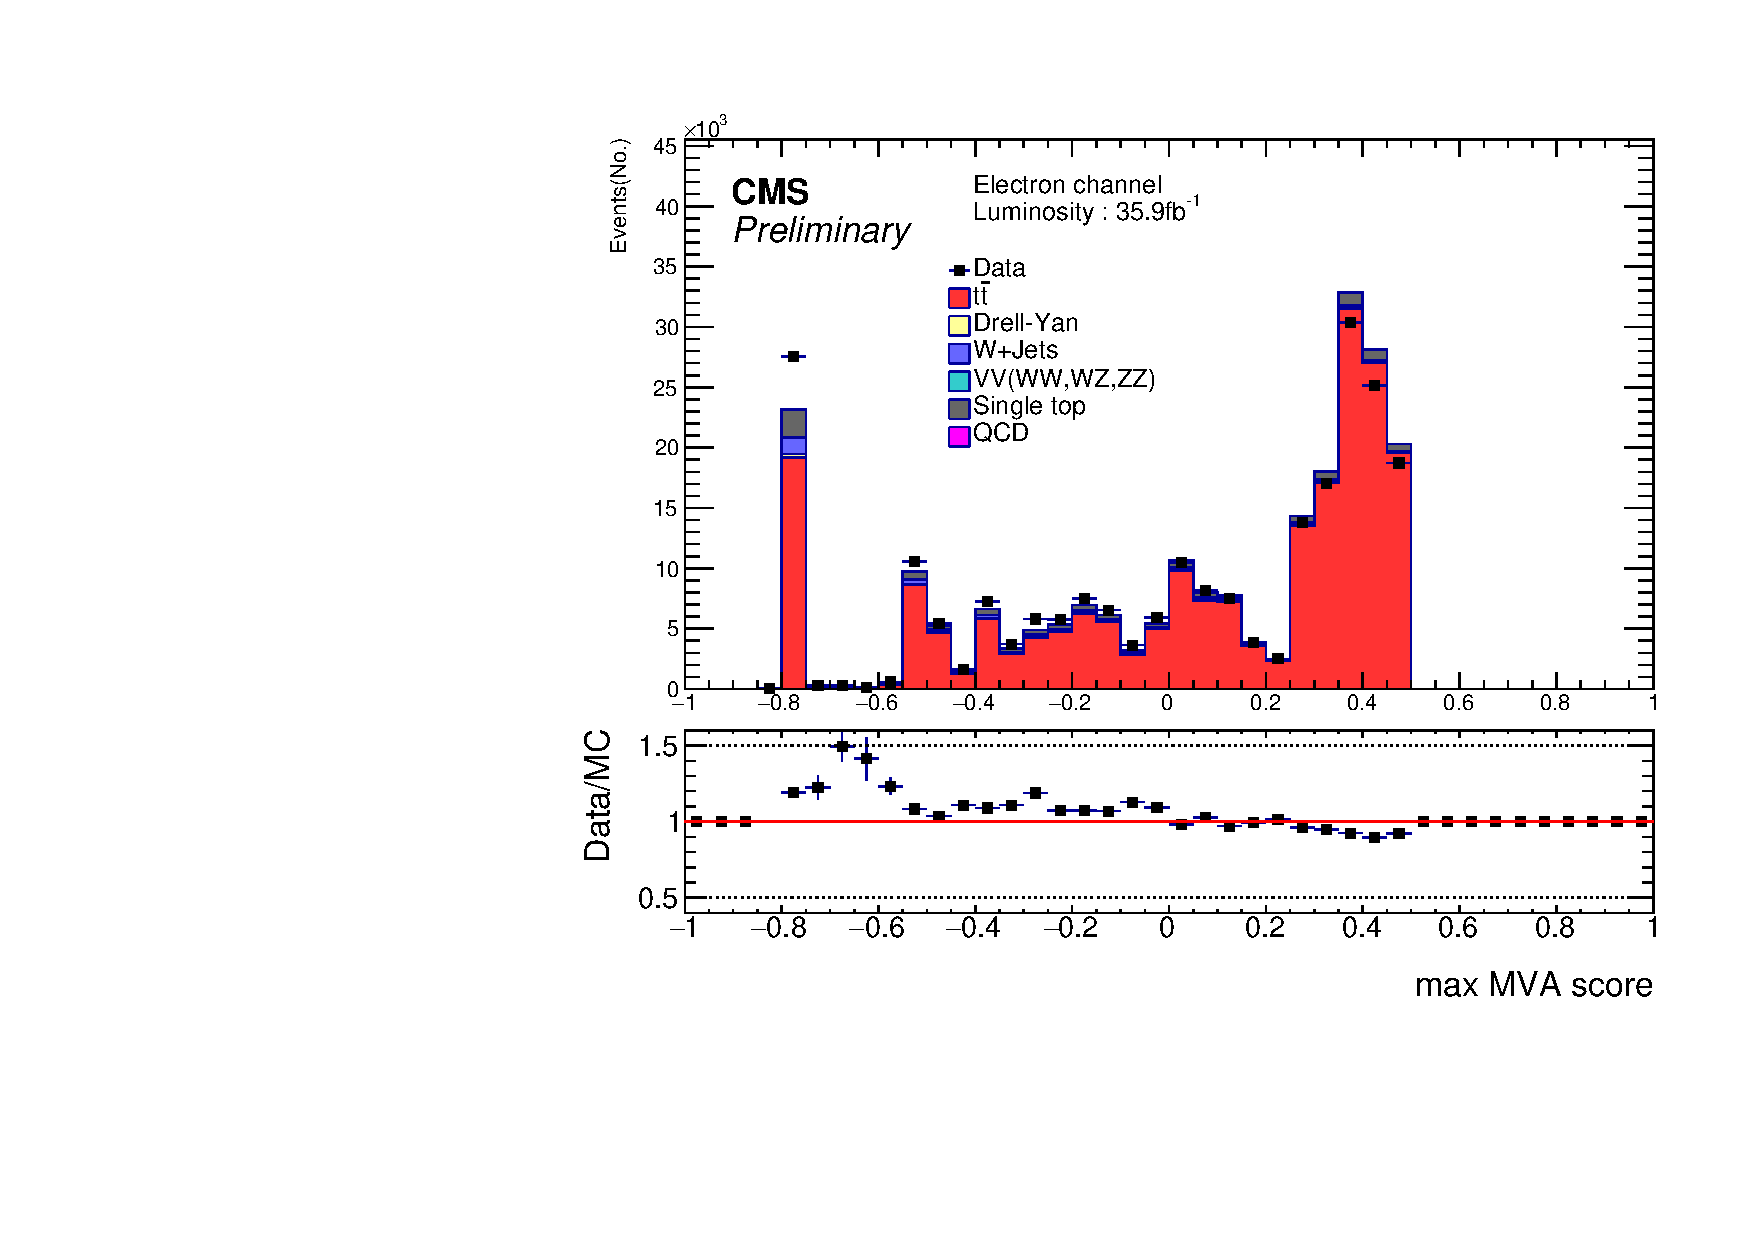
\includegraphics[width=0.32\textwidth]{Figures/EventSelReco/mva_algo/a04_BDT_SR_algo_el.pdf}}
			    \subfigure[BDTG (2 vars, el-ch)]{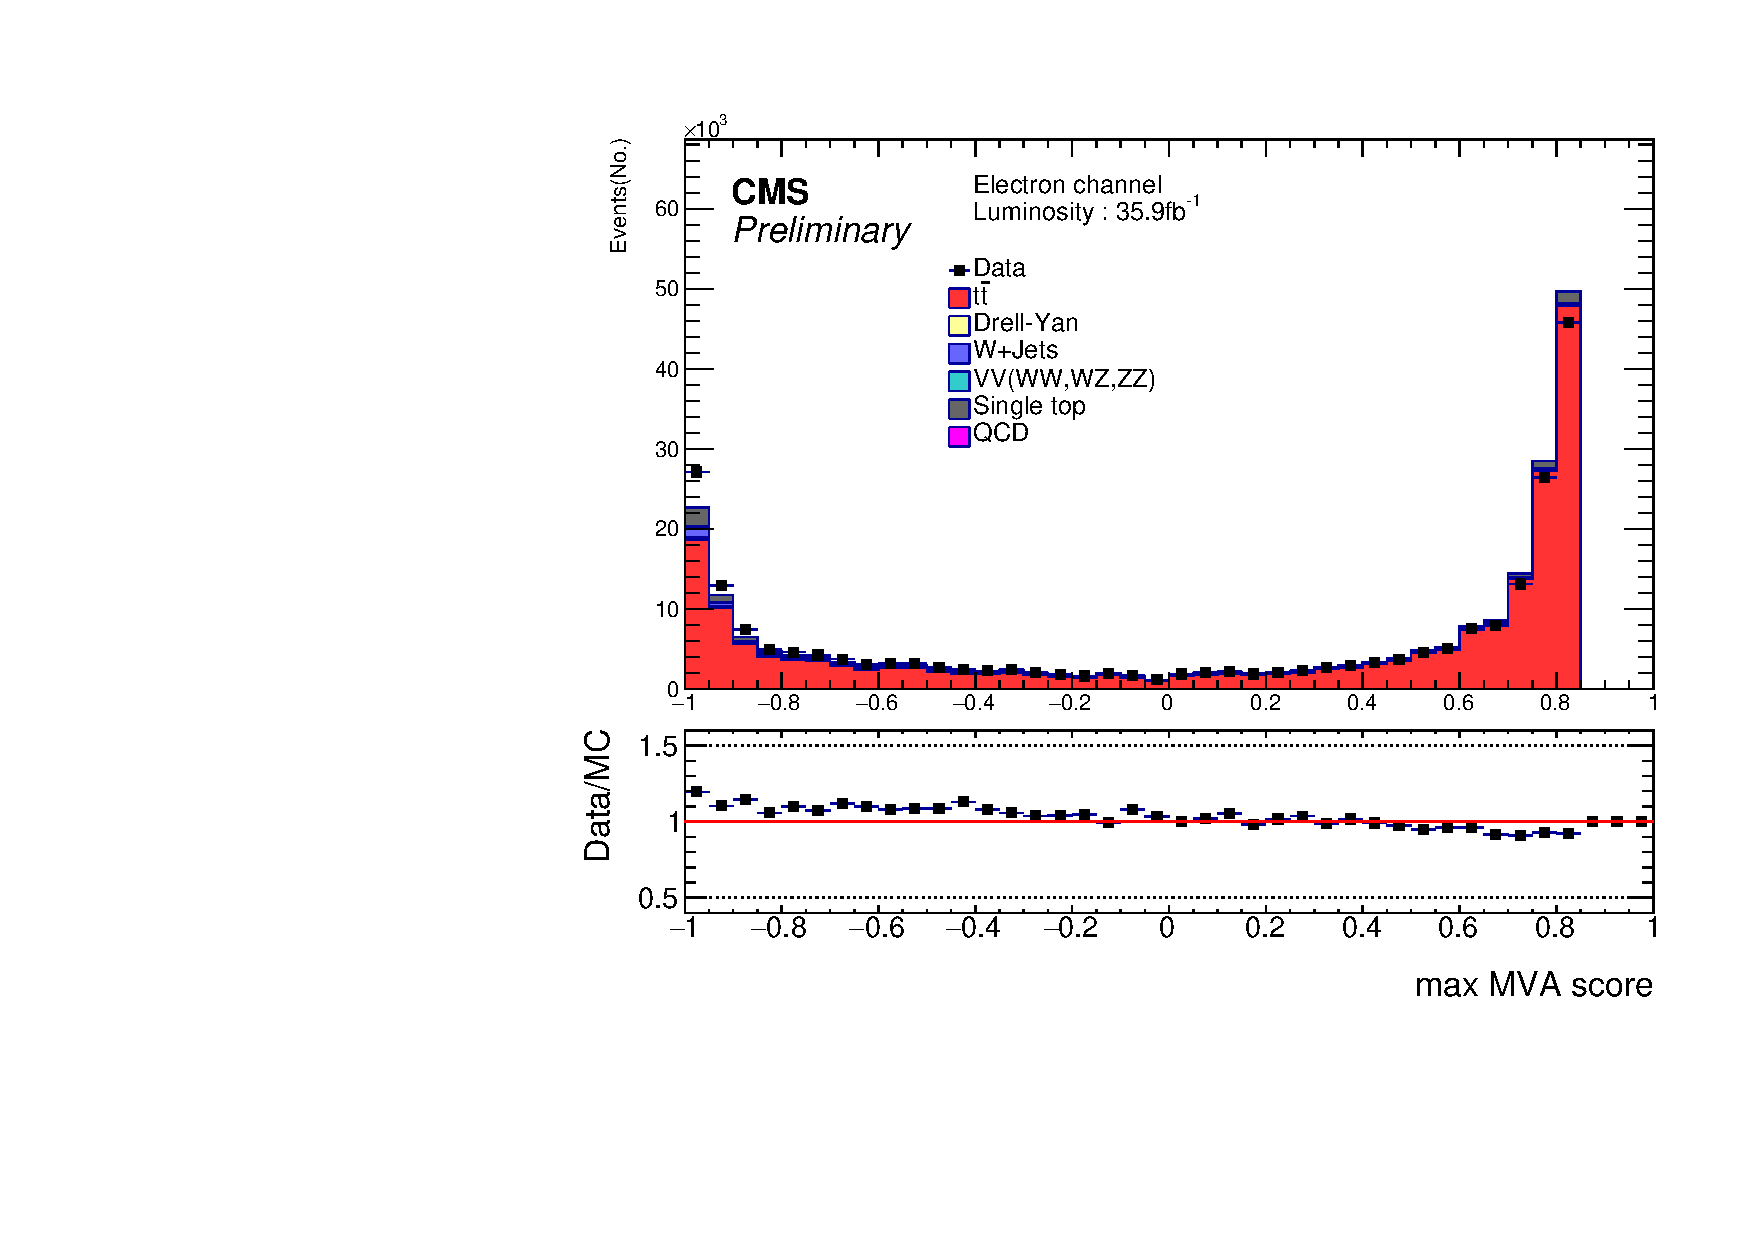
\includegraphics[width=0.32\textwidth]{Figures/EventSelReco/mva_algo/a04_BDTG_SR_algo_el.pdf}}
			    \subfigure[MLP (2 vars, el-ch)]{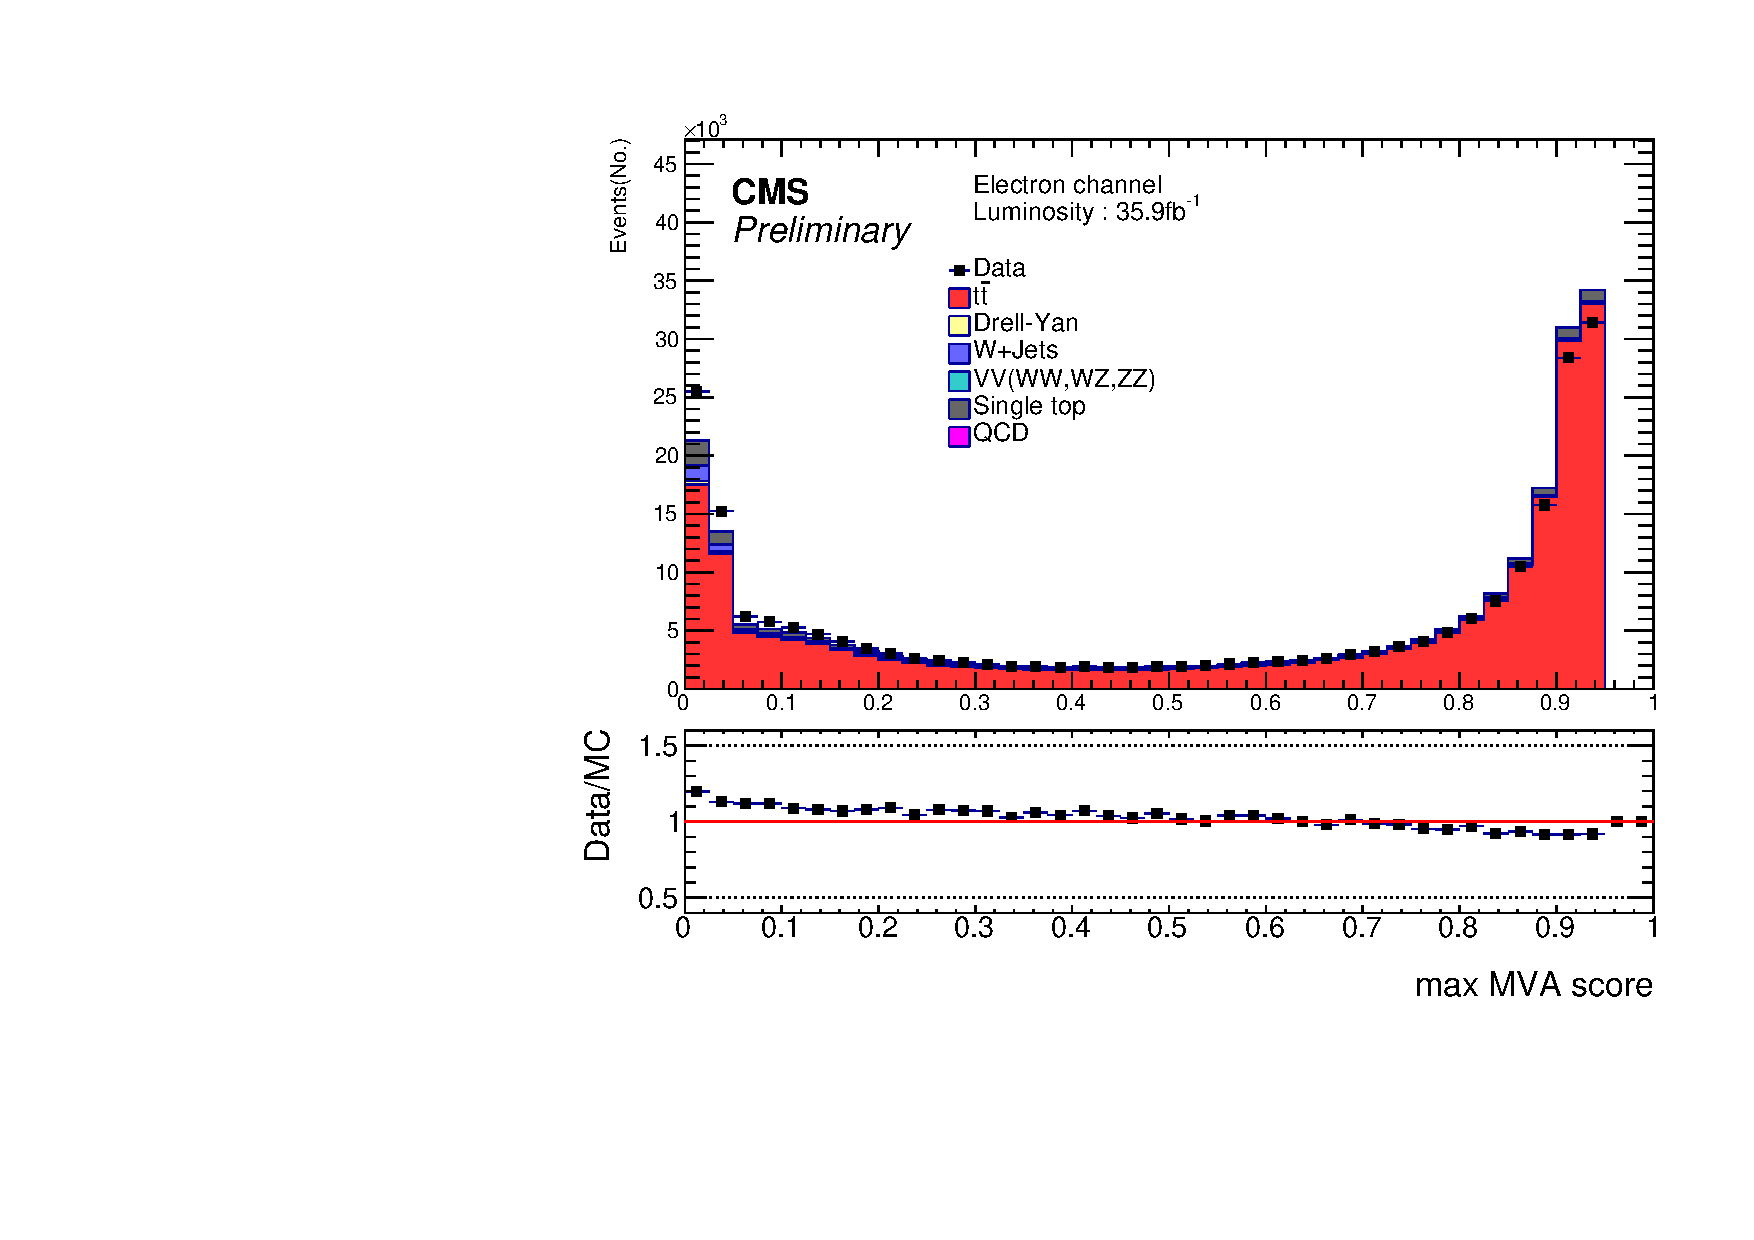
\includegraphics[width=0.32\textwidth]{Figures/EventSelReco/mva_algo/a04_MLP_SR_algo_el.pdf}}\\
			\caption{max MVA score in each event, comparing Data and MC.(2 variables training)}
			\label{EventSelReco:fig:a04_algo_DataMC}
			\end{figure}
			\FloatBarrier

			\begin{figure}[H]
			\centering
				\subfigure[BDT (8 vars, mu-ch)]{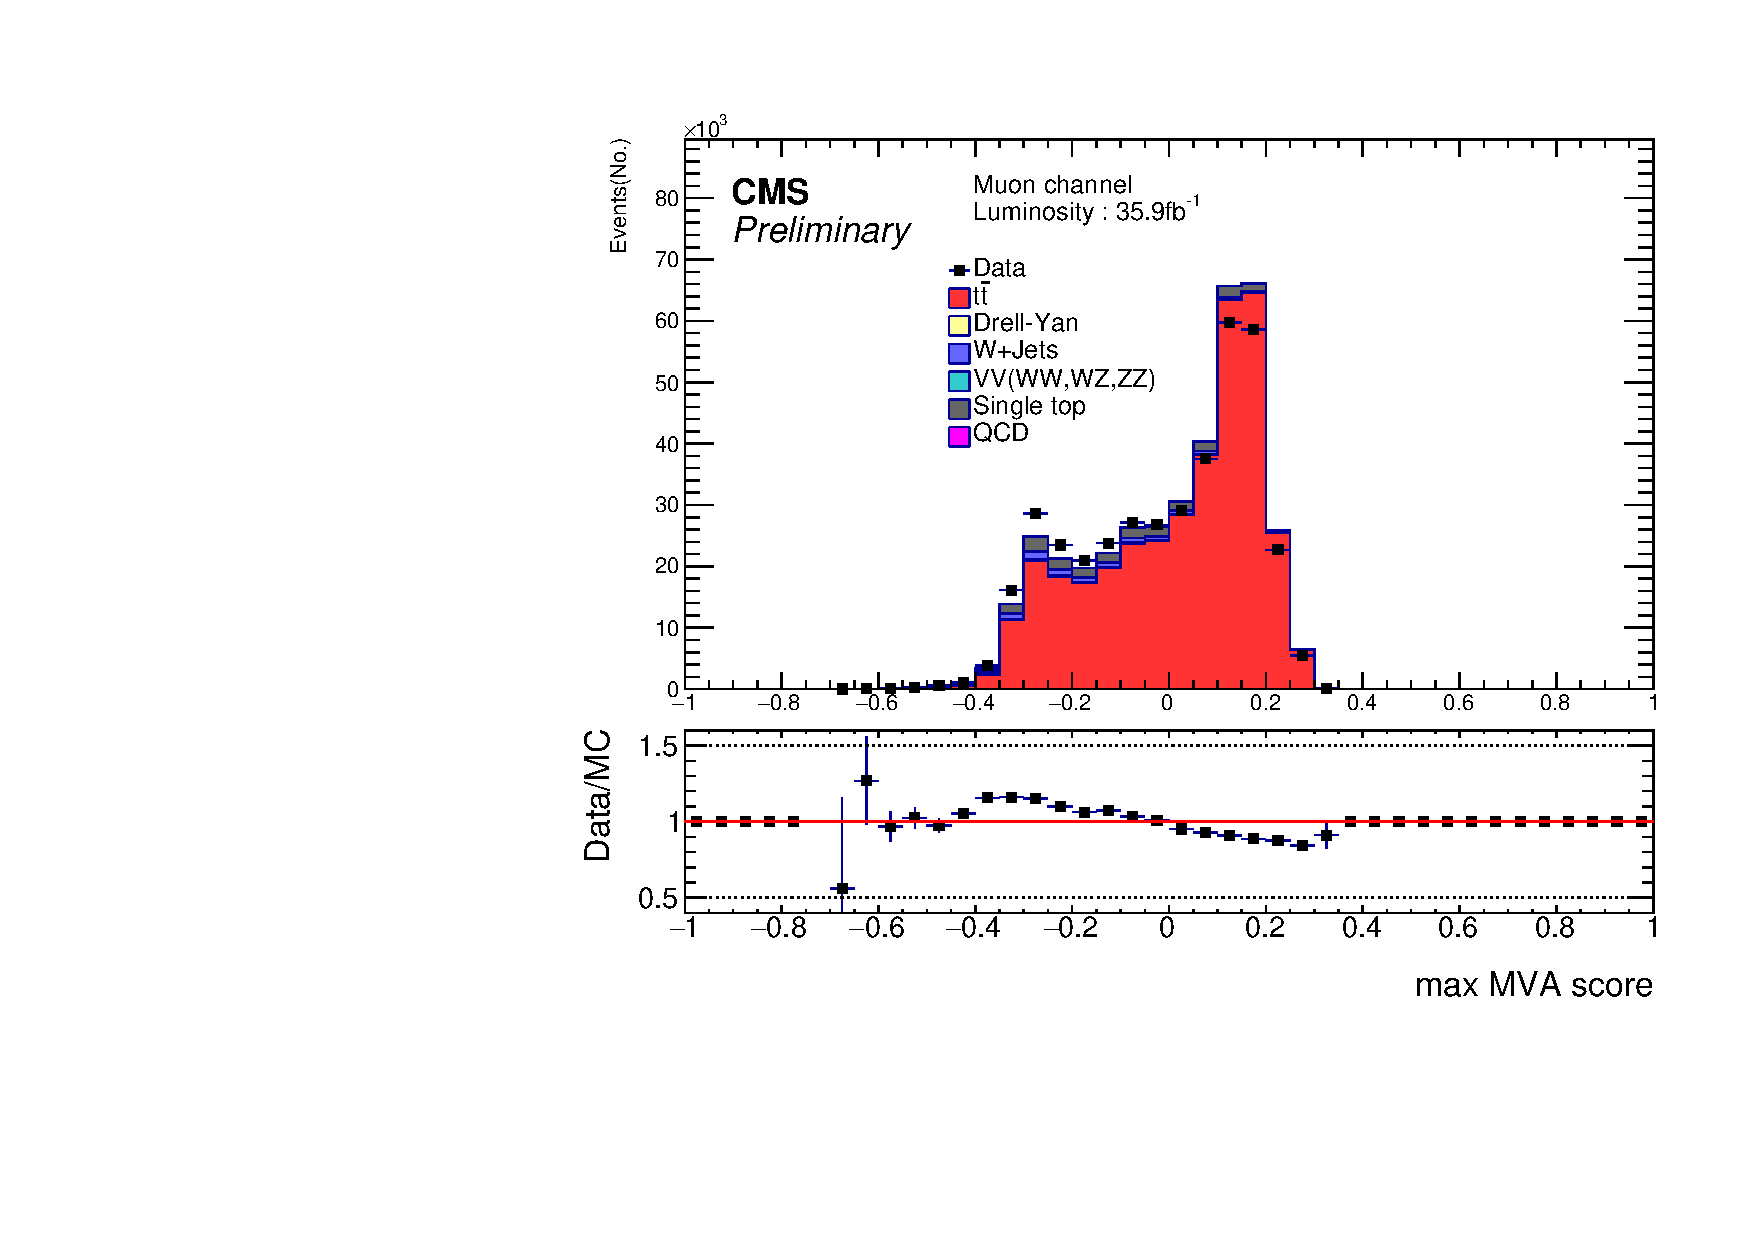
\includegraphics[width=0.32\textwidth]{Figures/EventSelReco/mva_algo/t13_BDT_SR_algo_mu.pdf}}
			    \subfigure[BDTG (8 vars, mu-ch)]{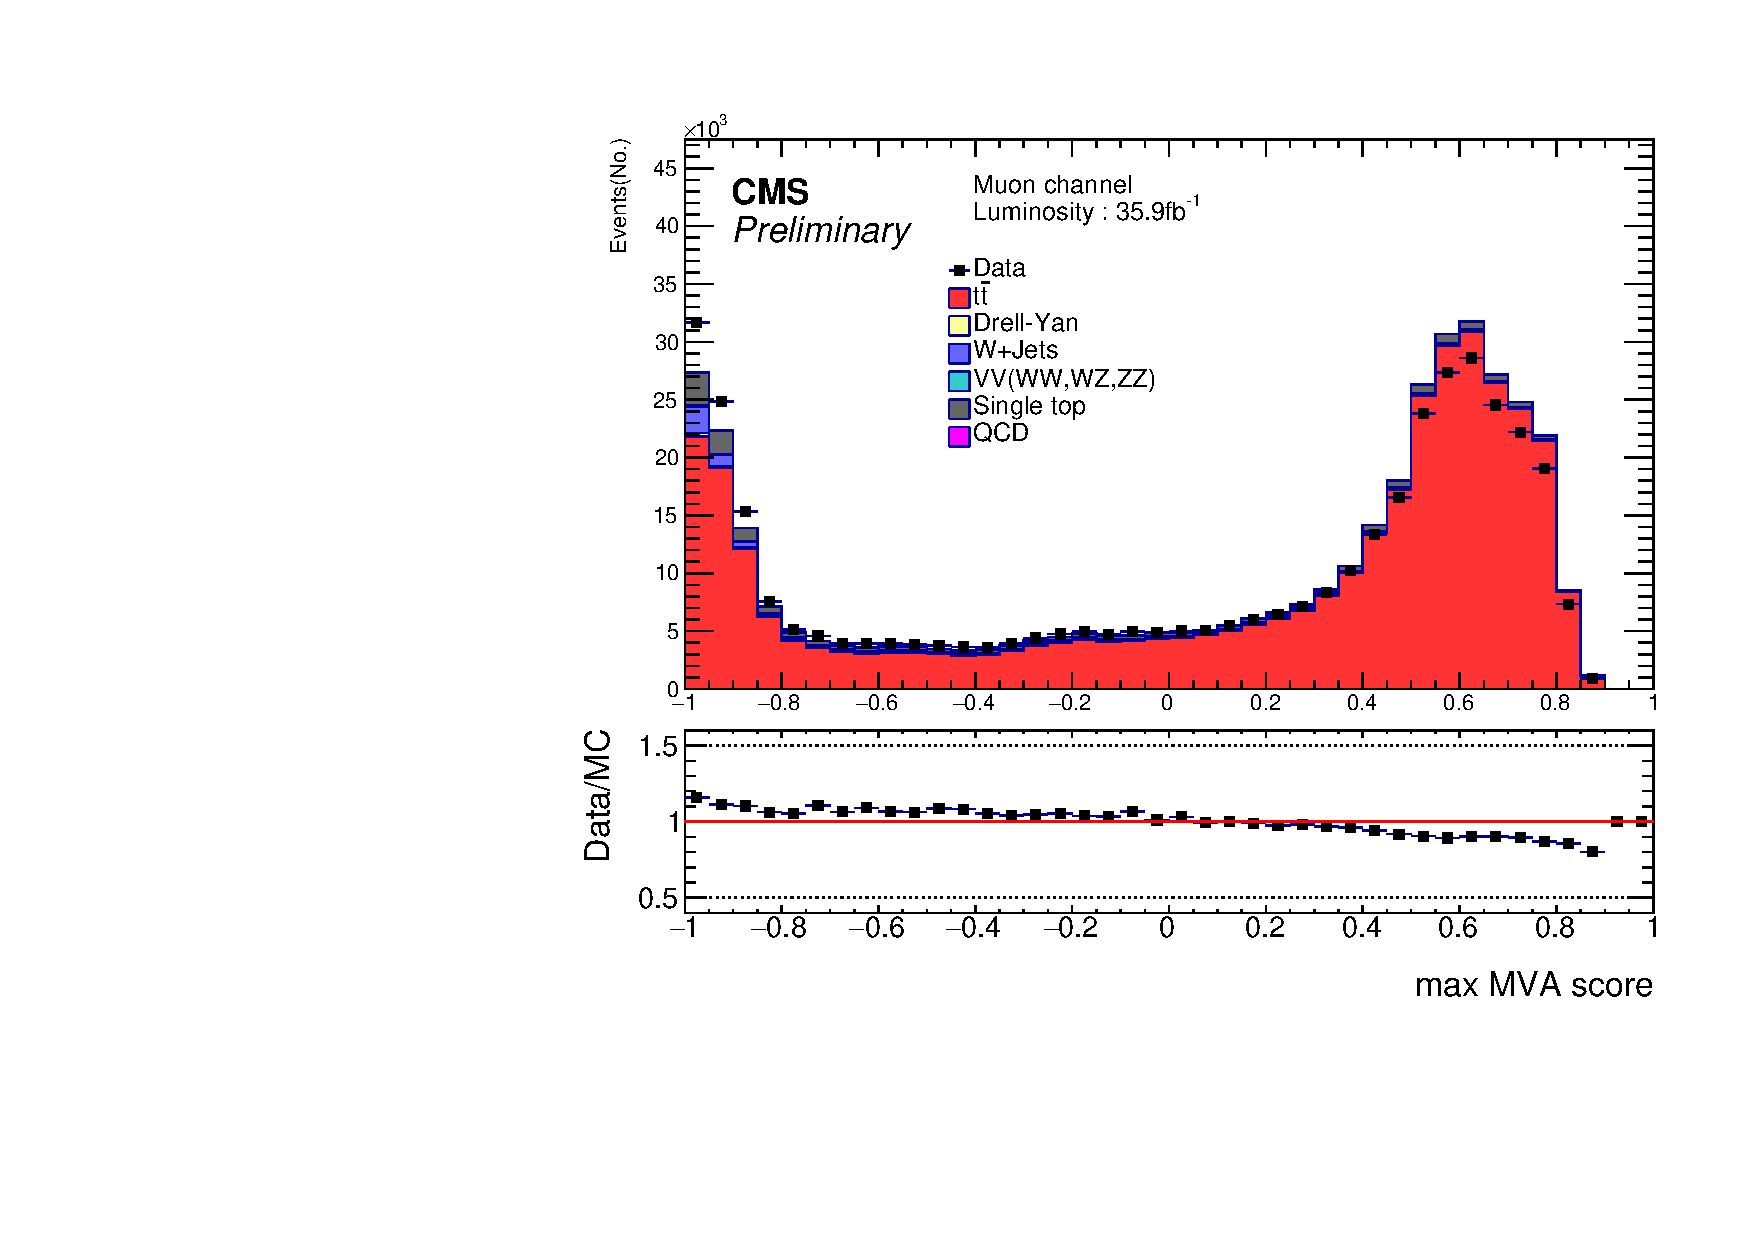
\includegraphics[width=0.32\textwidth]{Figures/EventSelReco/mva_algo/t13_BDTG_SR_algo_mu.pdf}}
			    \subfigure[MLP (8 vars, mu-ch)]{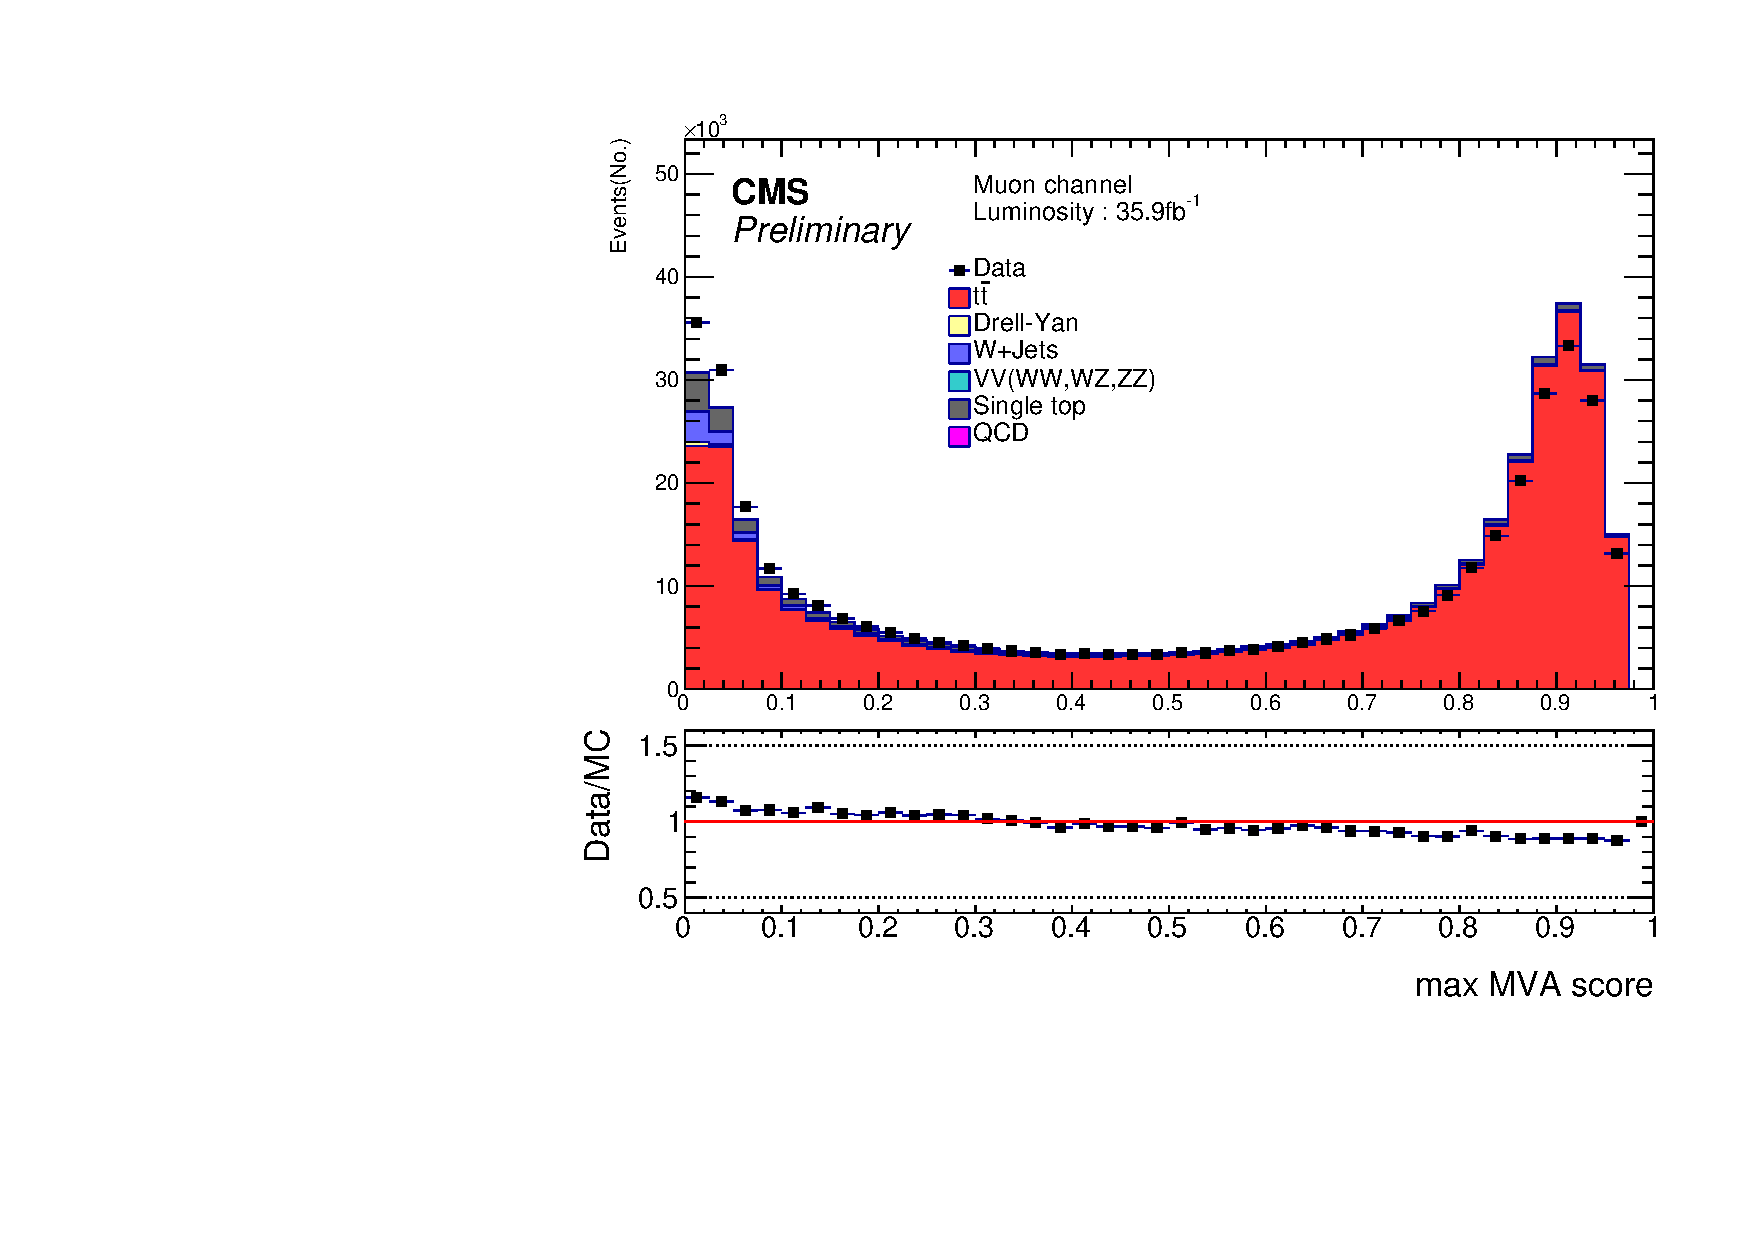
\includegraphics[width=0.32\textwidth]{Figures/EventSelReco/mva_algo/t13_MLP_SR_algo_mu.pdf}}\\			
			\end{figure}
			\FloatBarrier
			\begin{figure}[H]
			\centering
			    \subfigure[BDT (8 vars, el-ch)]{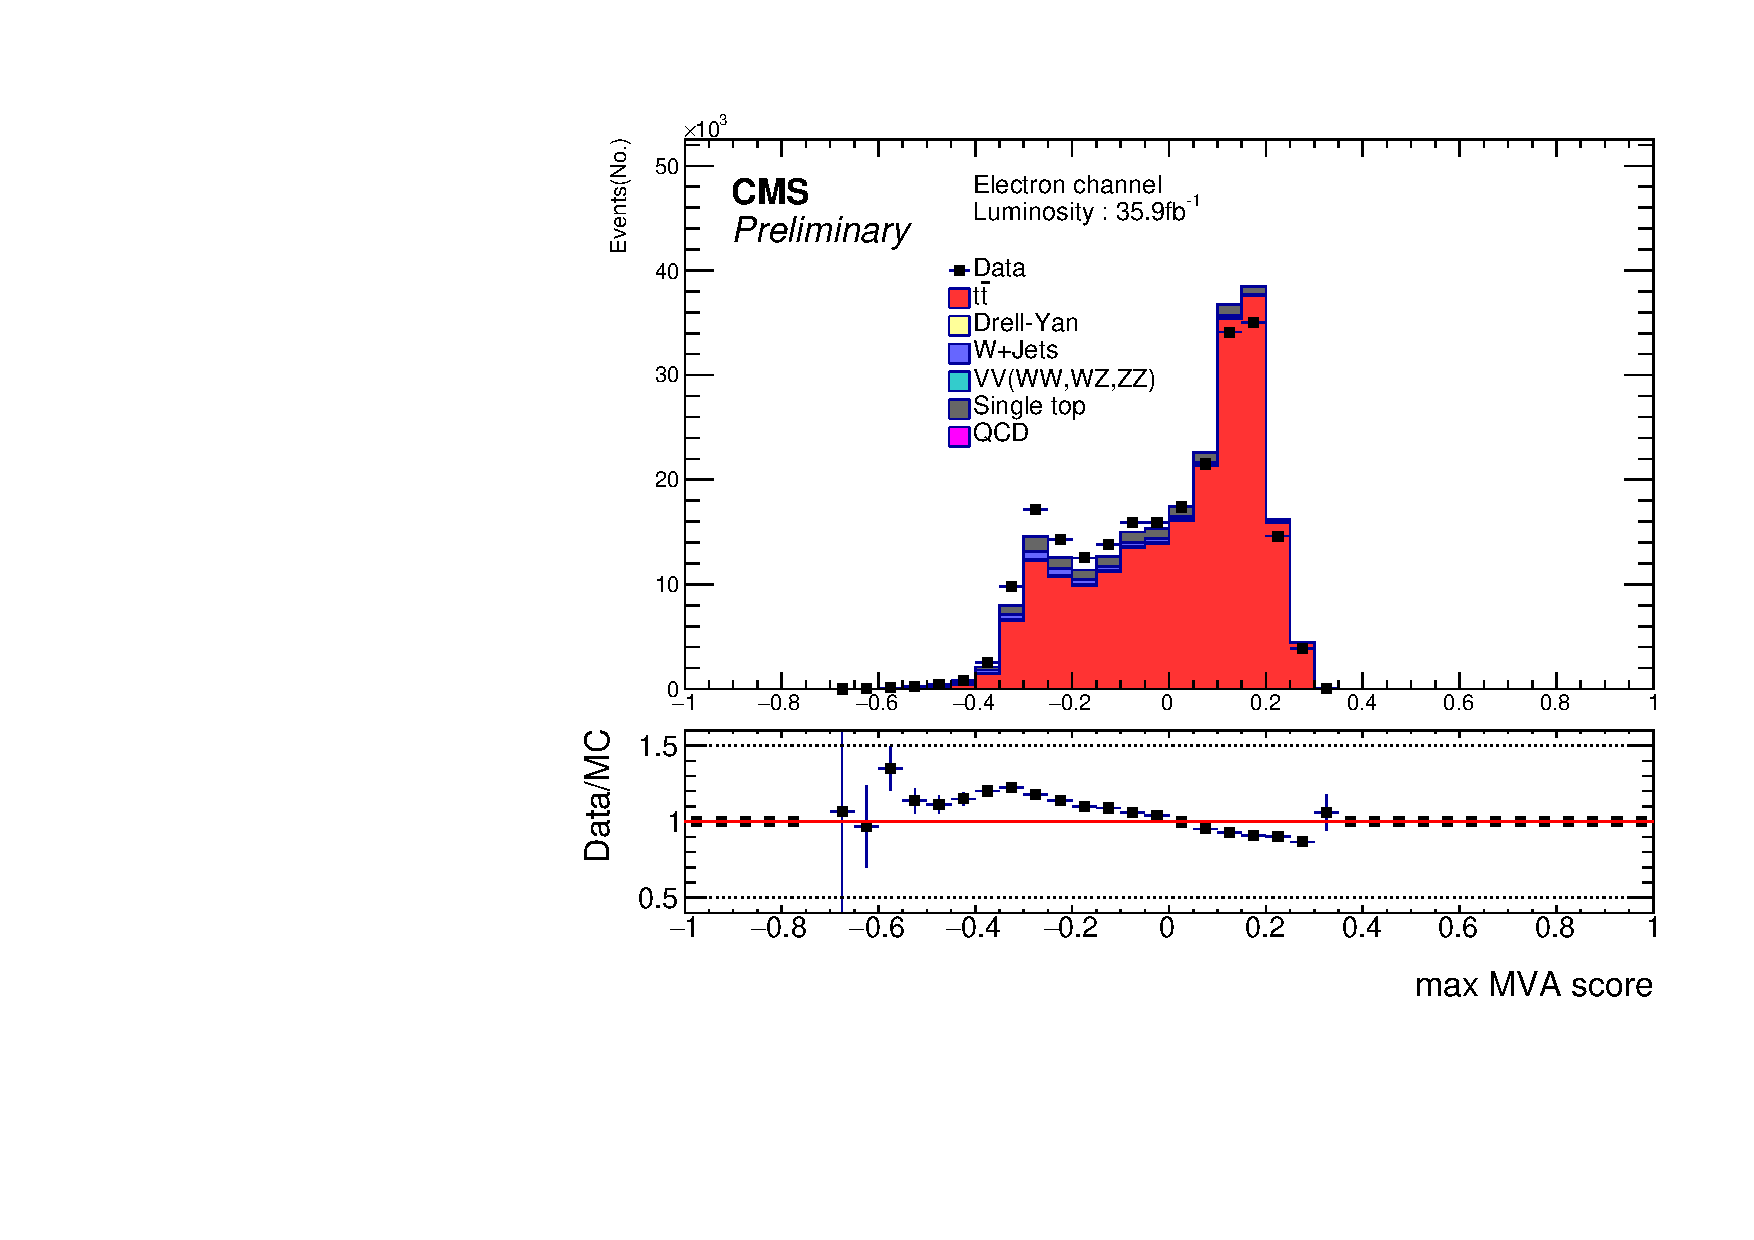
\includegraphics[width=0.32\textwidth]{Figures/EventSelReco/mva_algo/t13_BDT_SR_algo_el.pdf}}
			    \subfigure[BDTG (8 vars, el-ch)]{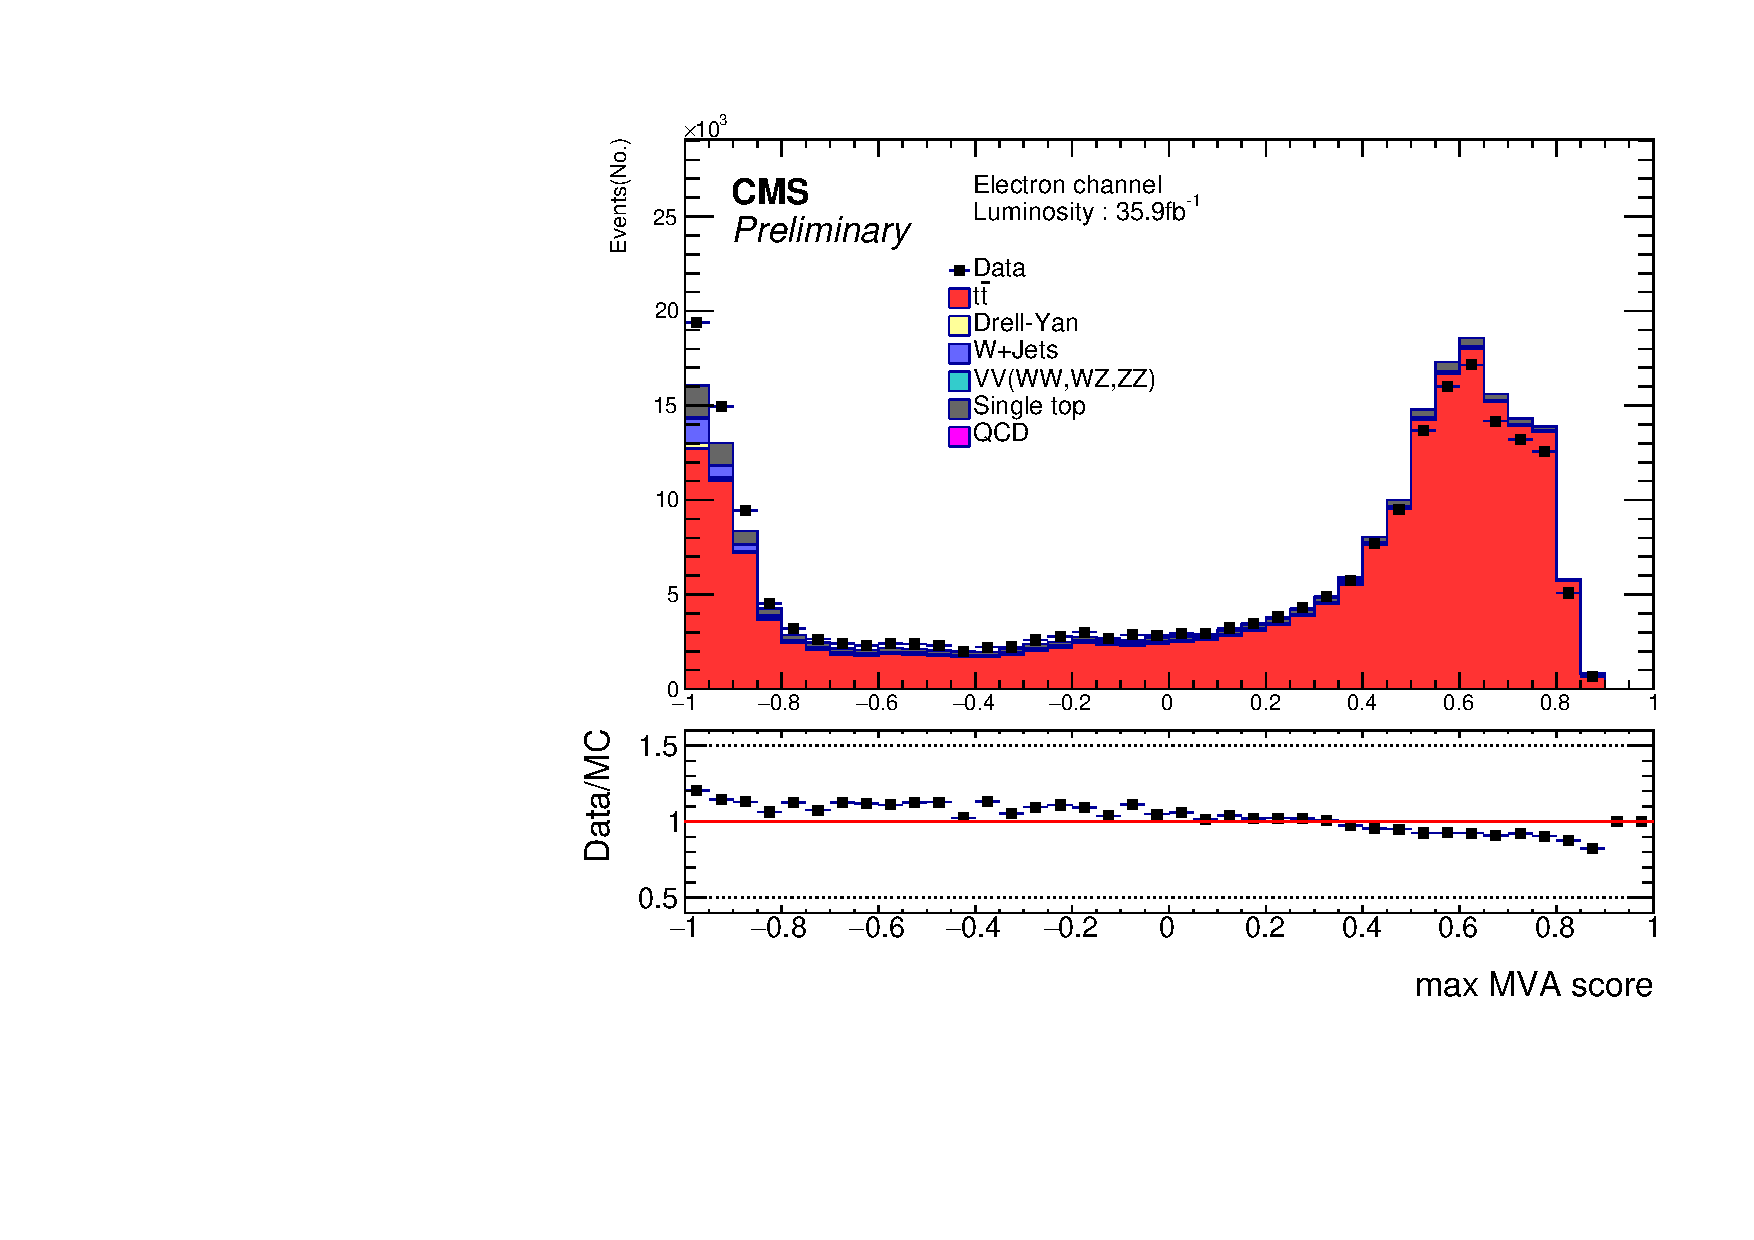
\includegraphics[width=0.32\textwidth]{Figures/EventSelReco/mva_algo/t13_BDTG_SR_algo_el.pdf}}
			    \subfigure[MLP (8 vars, el-ch)]{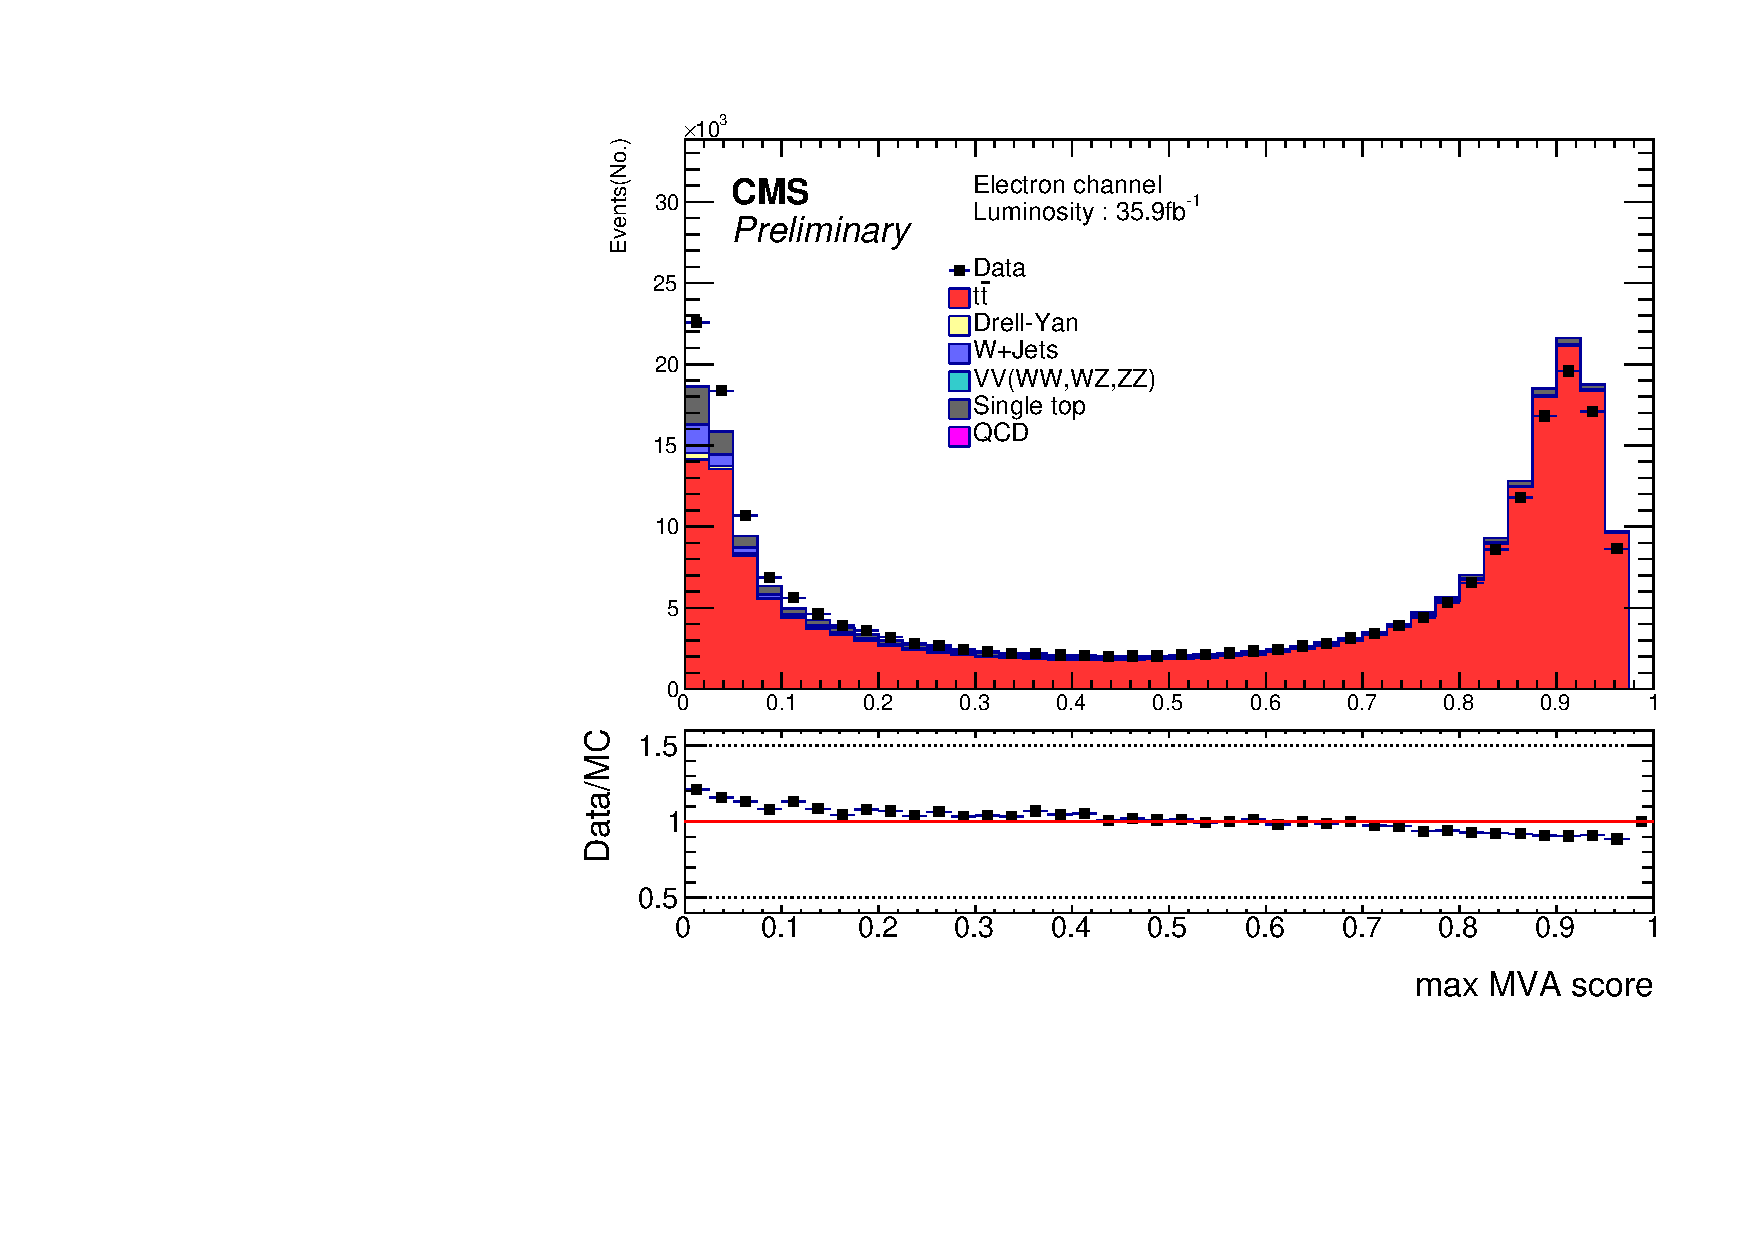
\includegraphics[width=0.32\textwidth]{Figures/EventSelReco/mva_algo/t13_MLP_SR_algo_el.pdf}}\\
			\caption{max MVA score in each event, comparing Data and MC.(8 variables training)}
			\label{EventSelReco:fig:t13_algo_DataMC}
			\end{figure}
			\FloatBarrier

			\begin{figure}[H]
			\centering
				\subfigure[BDT (20 vars, mu-ch)]{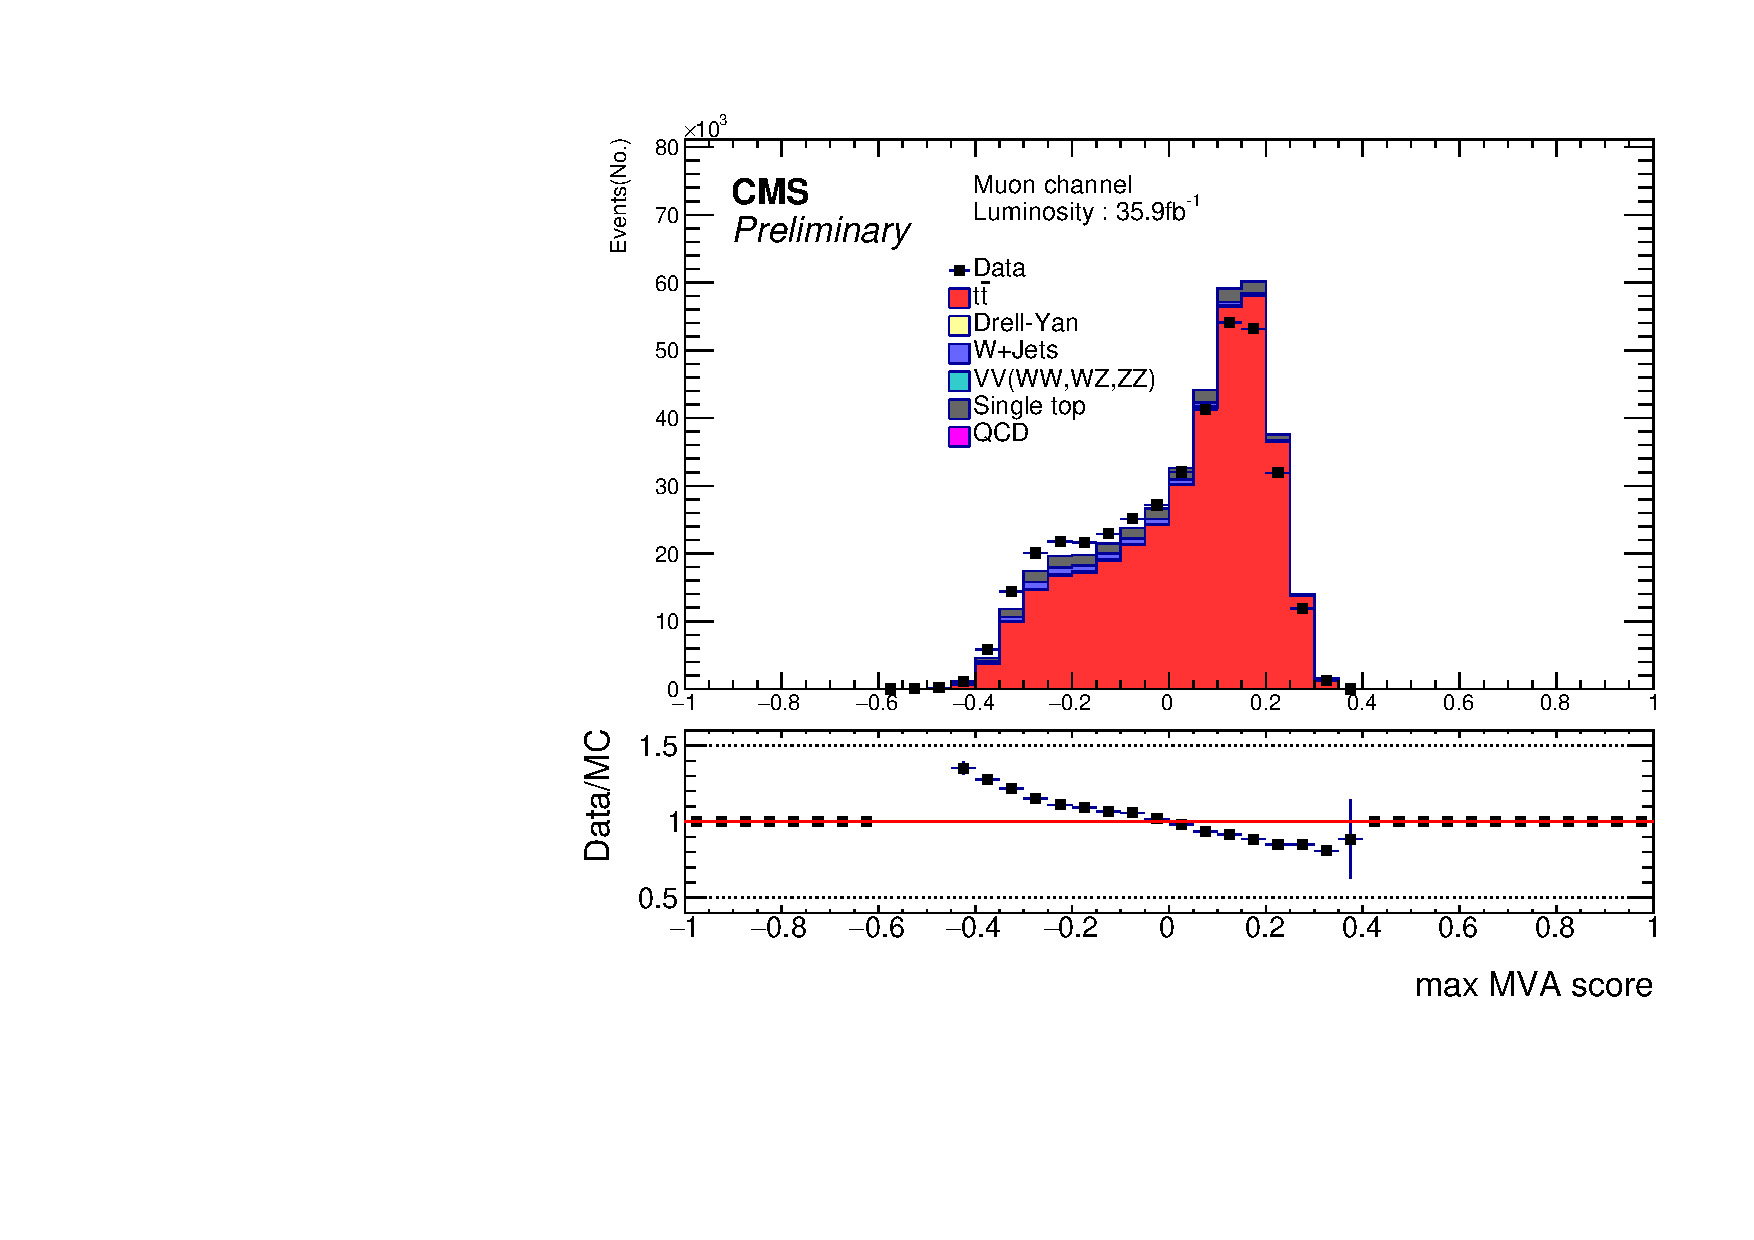
\includegraphics[width=0.32\textwidth]{Figures/EventSelReco/mva_algo/a05_BDT_SR_algo_mu.pdf}}
			    \subfigure[BDTG (20 vars, mu-ch)]{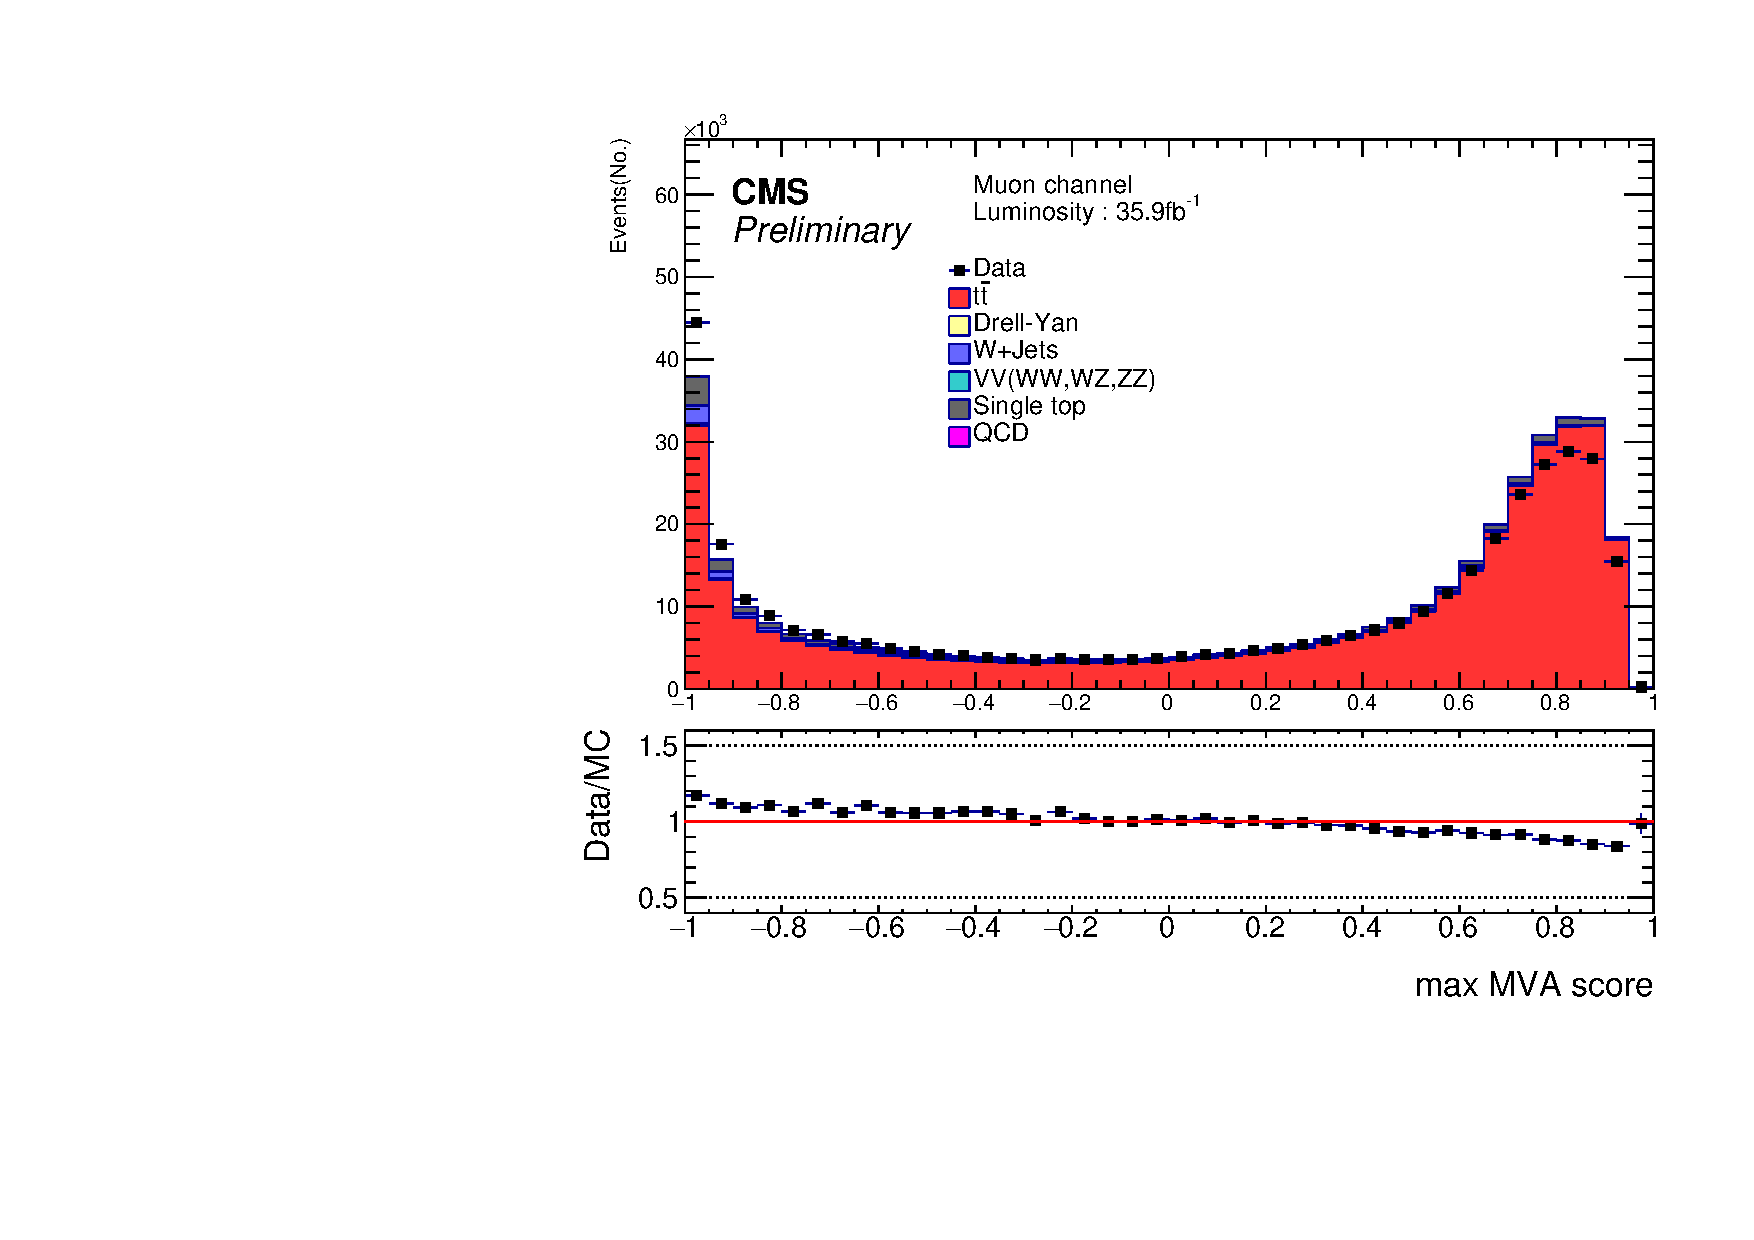
\includegraphics[width=0.32\textwidth]{Figures/EventSelReco/mva_algo/a05_BDTG_SR_algo_mu.pdf}}
			    \subfigure[MLP (20 vars, mu-ch)]{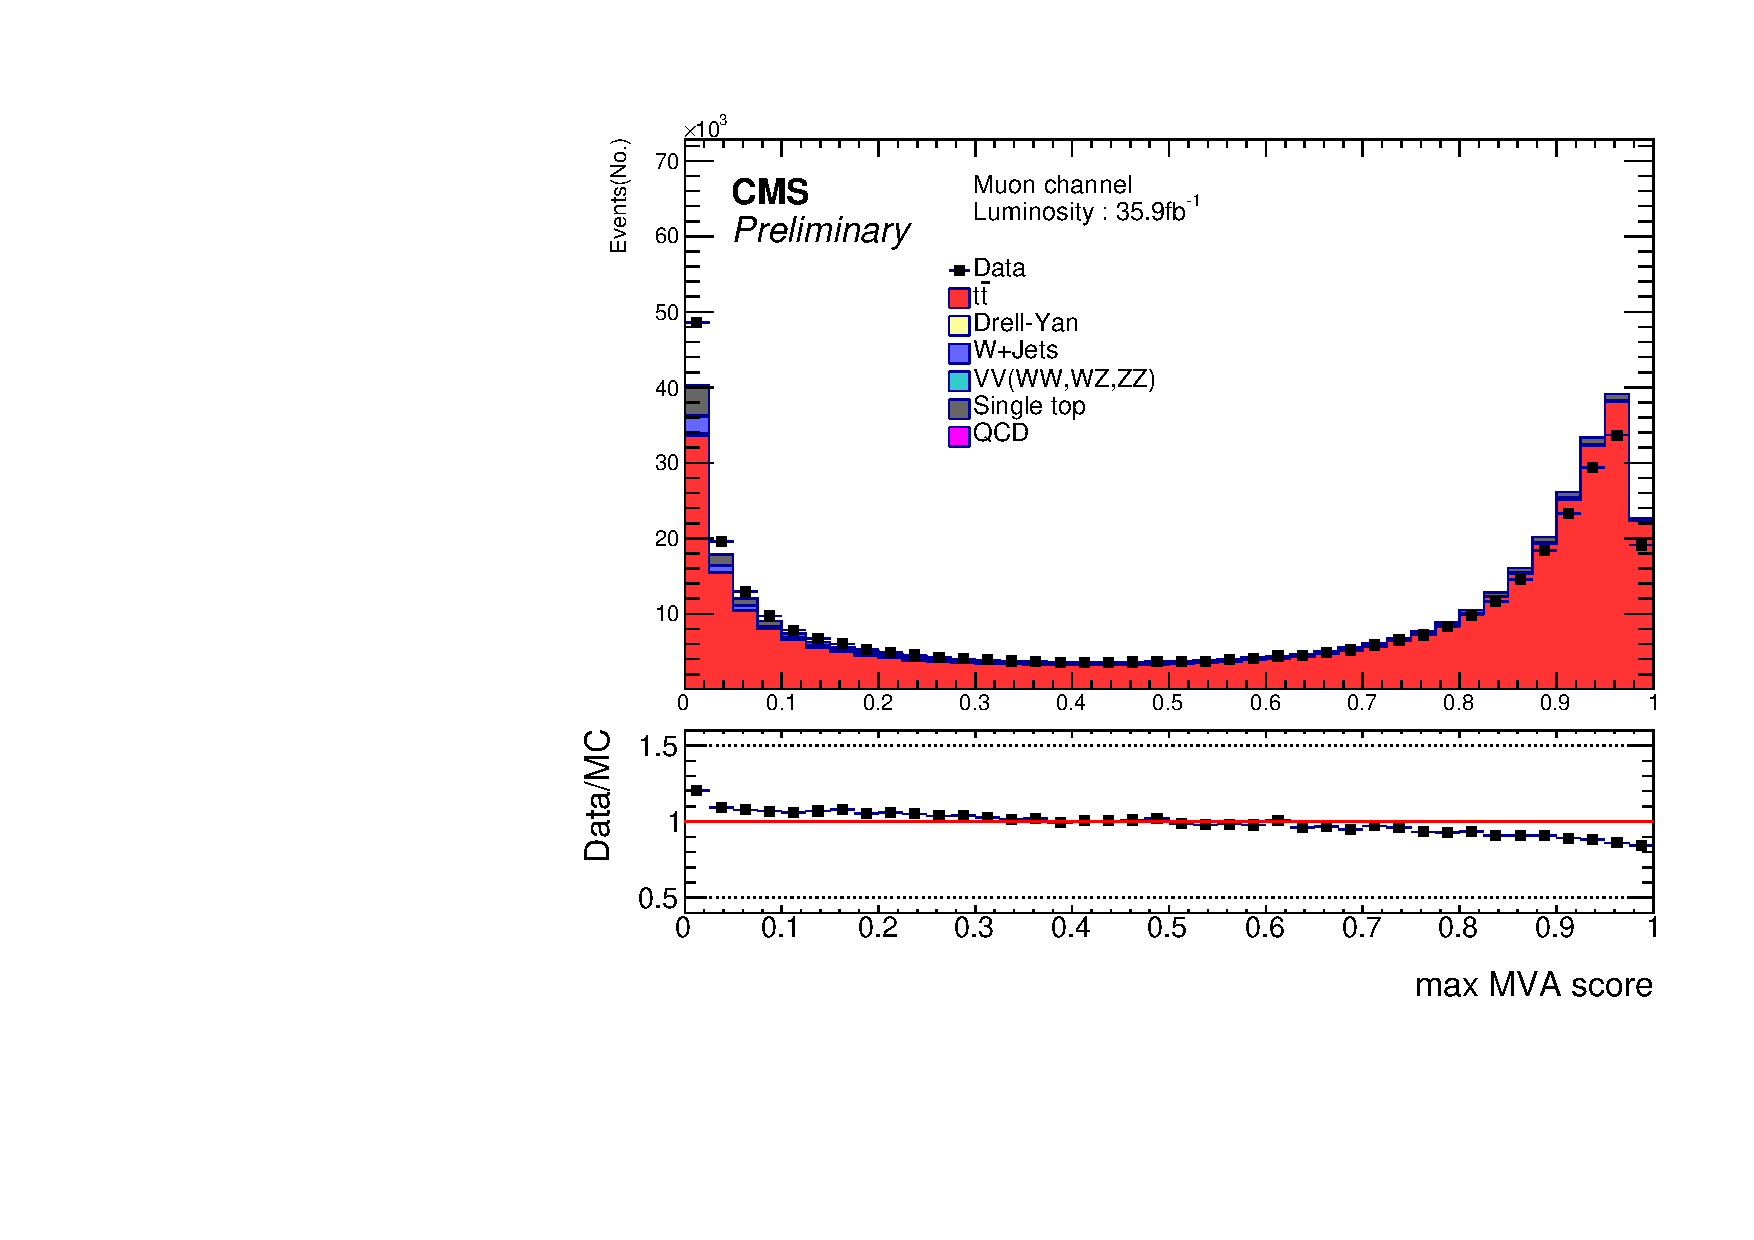
\includegraphics[width=0.32\textwidth]{Figures/EventSelReco/mva_algo/a05_MLP_SR_algo_mu.pdf}}\\
			\end{figure}
			\FloatBarrier
			\begin{figure}[H]
			\centering
			    \subfigure[BDT (20 vars, el-ch)]{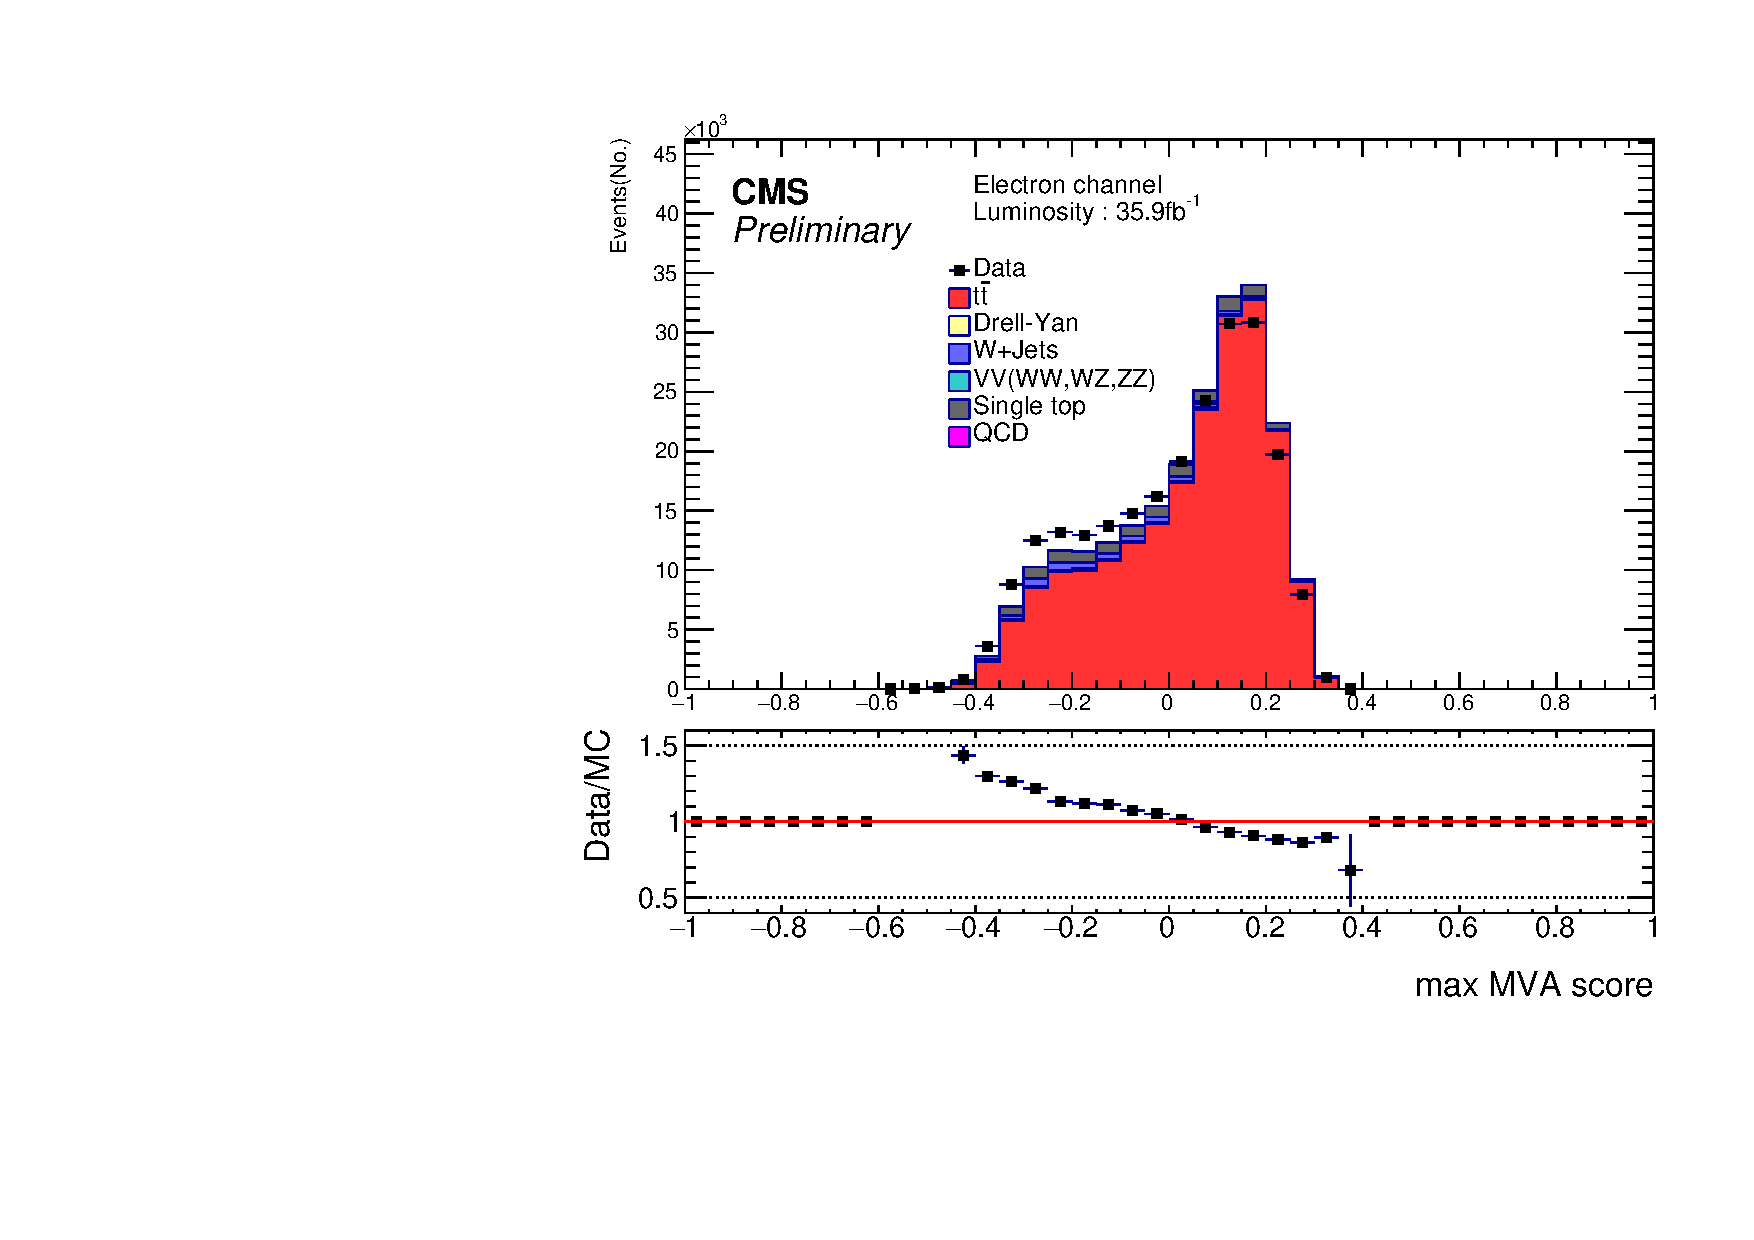
\includegraphics[width=0.32\textwidth]{Figures/EventSelReco/mva_algo/a05_BDT_SR_algo_el.pdf}}
			    \subfigure[BDTG (20 vars, el-ch)]{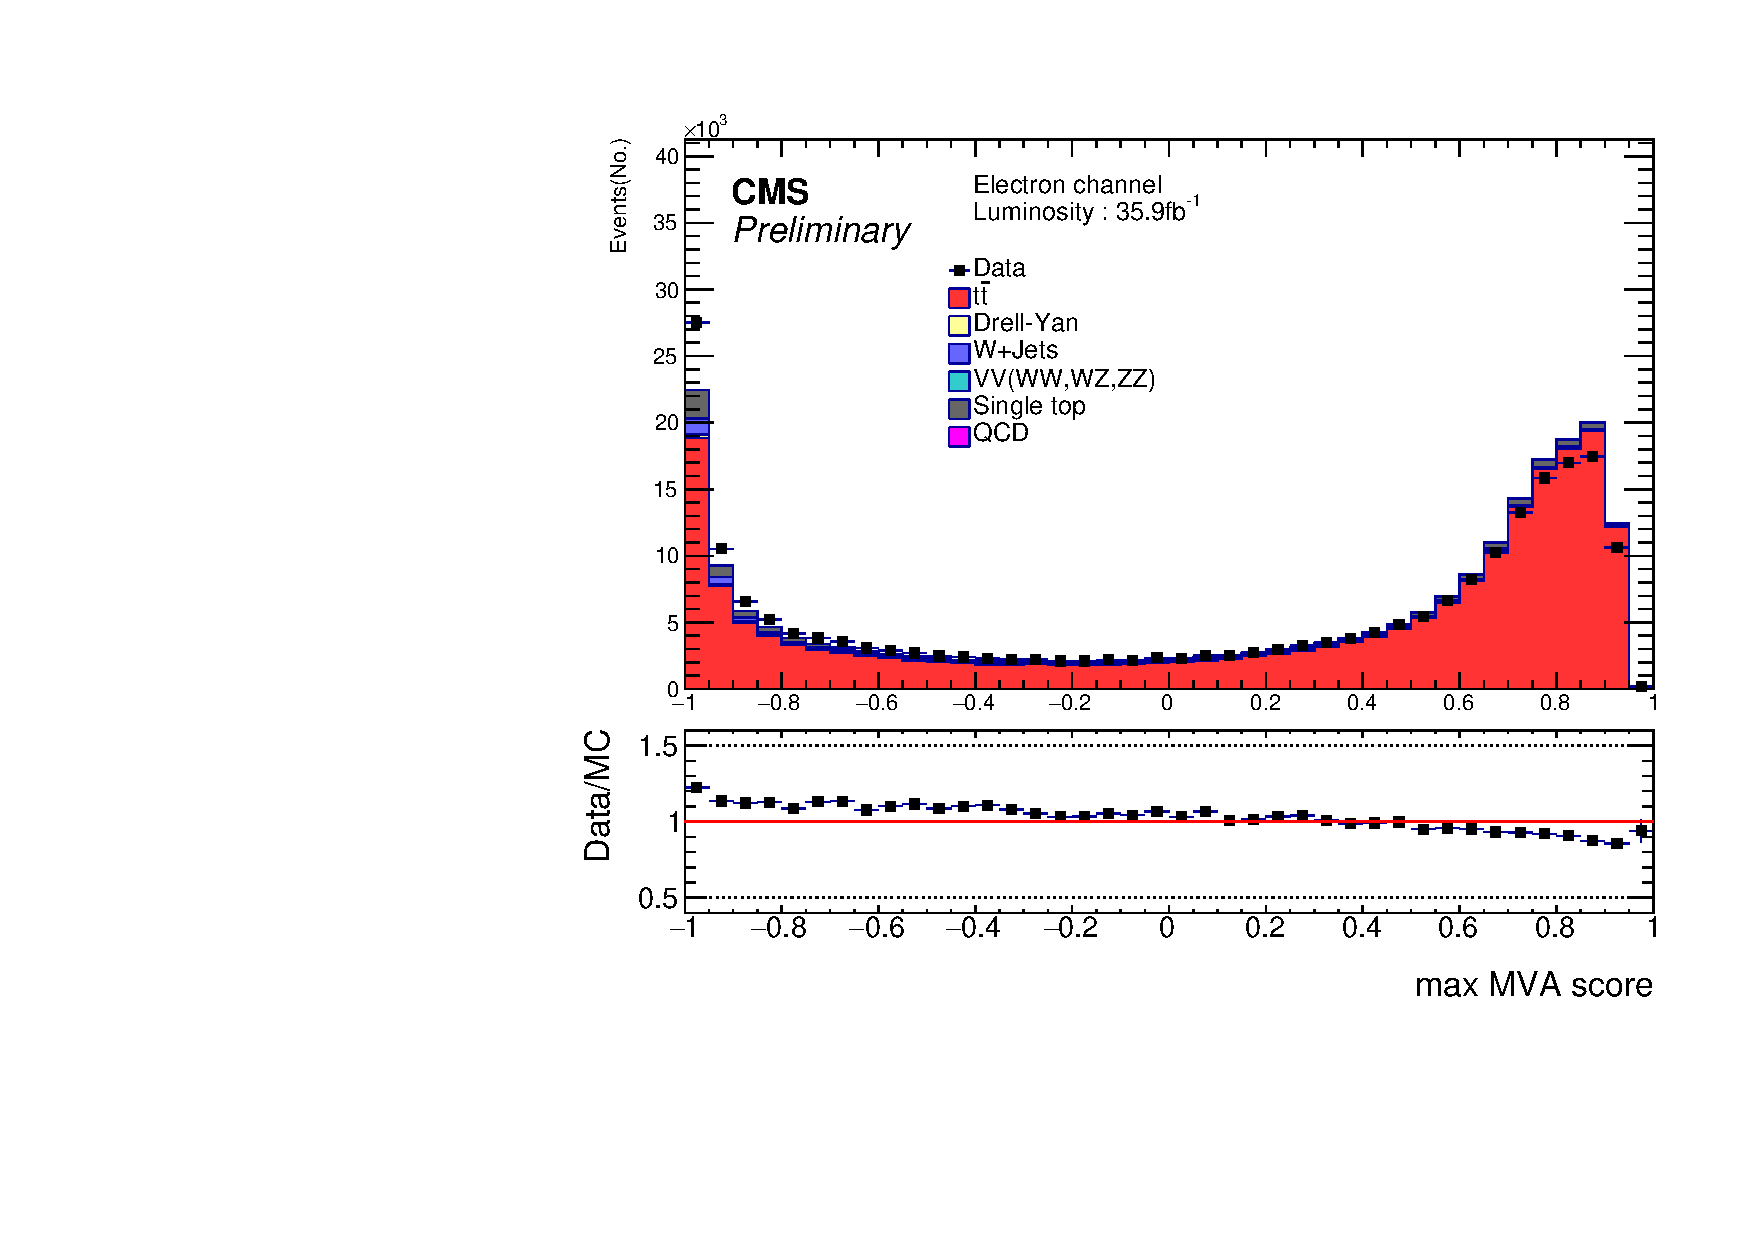
\includegraphics[width=0.32\textwidth]{Figures/EventSelReco/mva_algo/a05_BDTG_SR_algo_el.pdf}}
			    \subfigure[MLP (20 vars, el-ch)]{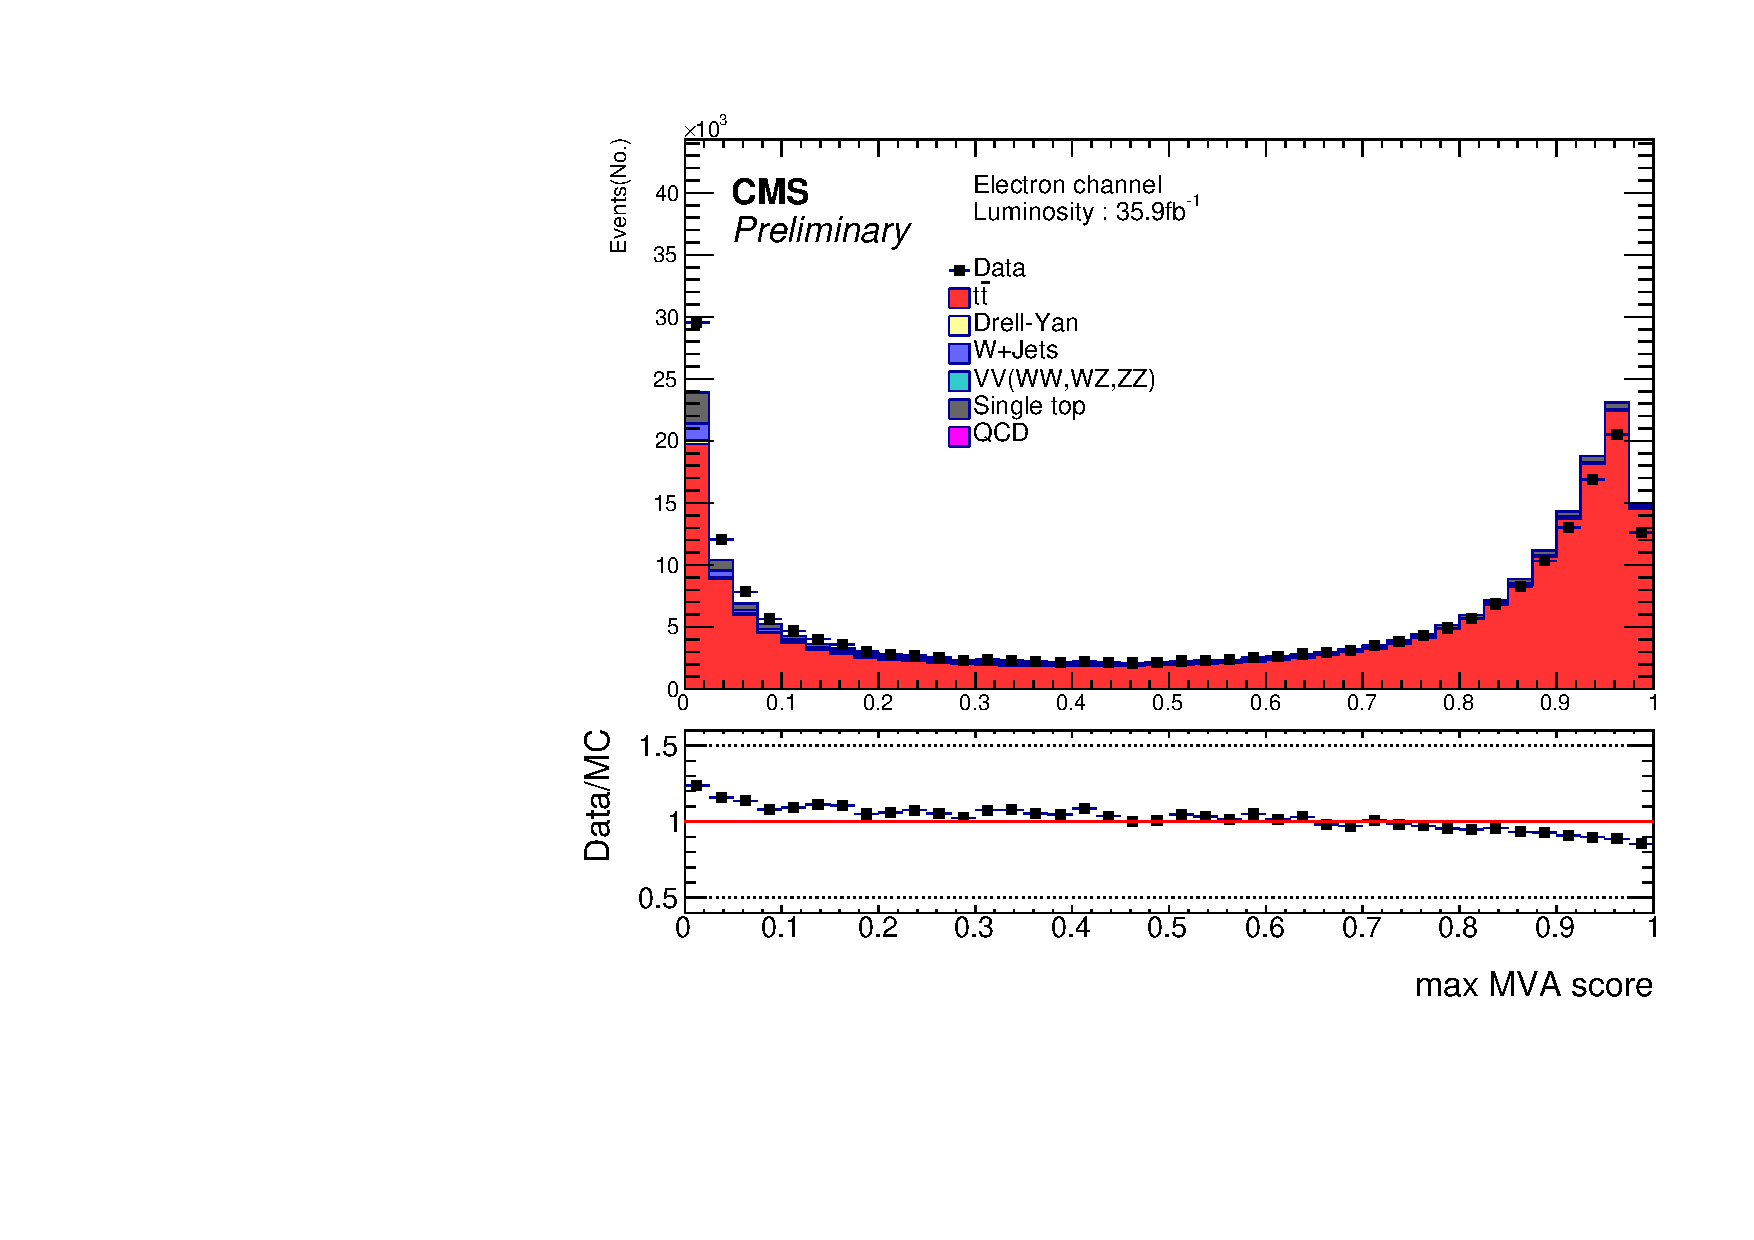
\includegraphics[width=0.32\textwidth]{Figures/EventSelReco/mva_algo/a05_MLP_SR_algo_el.pdf}}\\
			\caption{max MVA score in each event, comparing Data and MC.(20 variables training)}
			\label{EventSelReco:fig:a05_algo_DataMC}
			\end{figure}
			\FloatBarrier

			%%% In the Fig.\ref{EventSelReco:fig:a04_algo_DataMC_mu} $\sim$ Fig.\ref{EventSelReco:fig:a05_algo_DataMC_el}, we can see that at the low and high max MVA score region, there is a little discrecpancy. It probably comes from the jet characteristic of jets multiplicity between Data and MC. In real data, there would be more soft jets than simulation(MC) sample. On the basis of number of jets, there are more probable combinations of jjb in data. It means that the max MVA value is more probable at low value in data. That is a possibility of the discrepancy.

			The training variables may have correlation with each other. If there are too much characteristic to be trained alike between variables, the most of input informations would duplicate. To check the variables' correlation score is necessary: (20 variables' case is shown)

			\begin{figure}[H]
			\centering
			    \subfigure[Variables in signal]{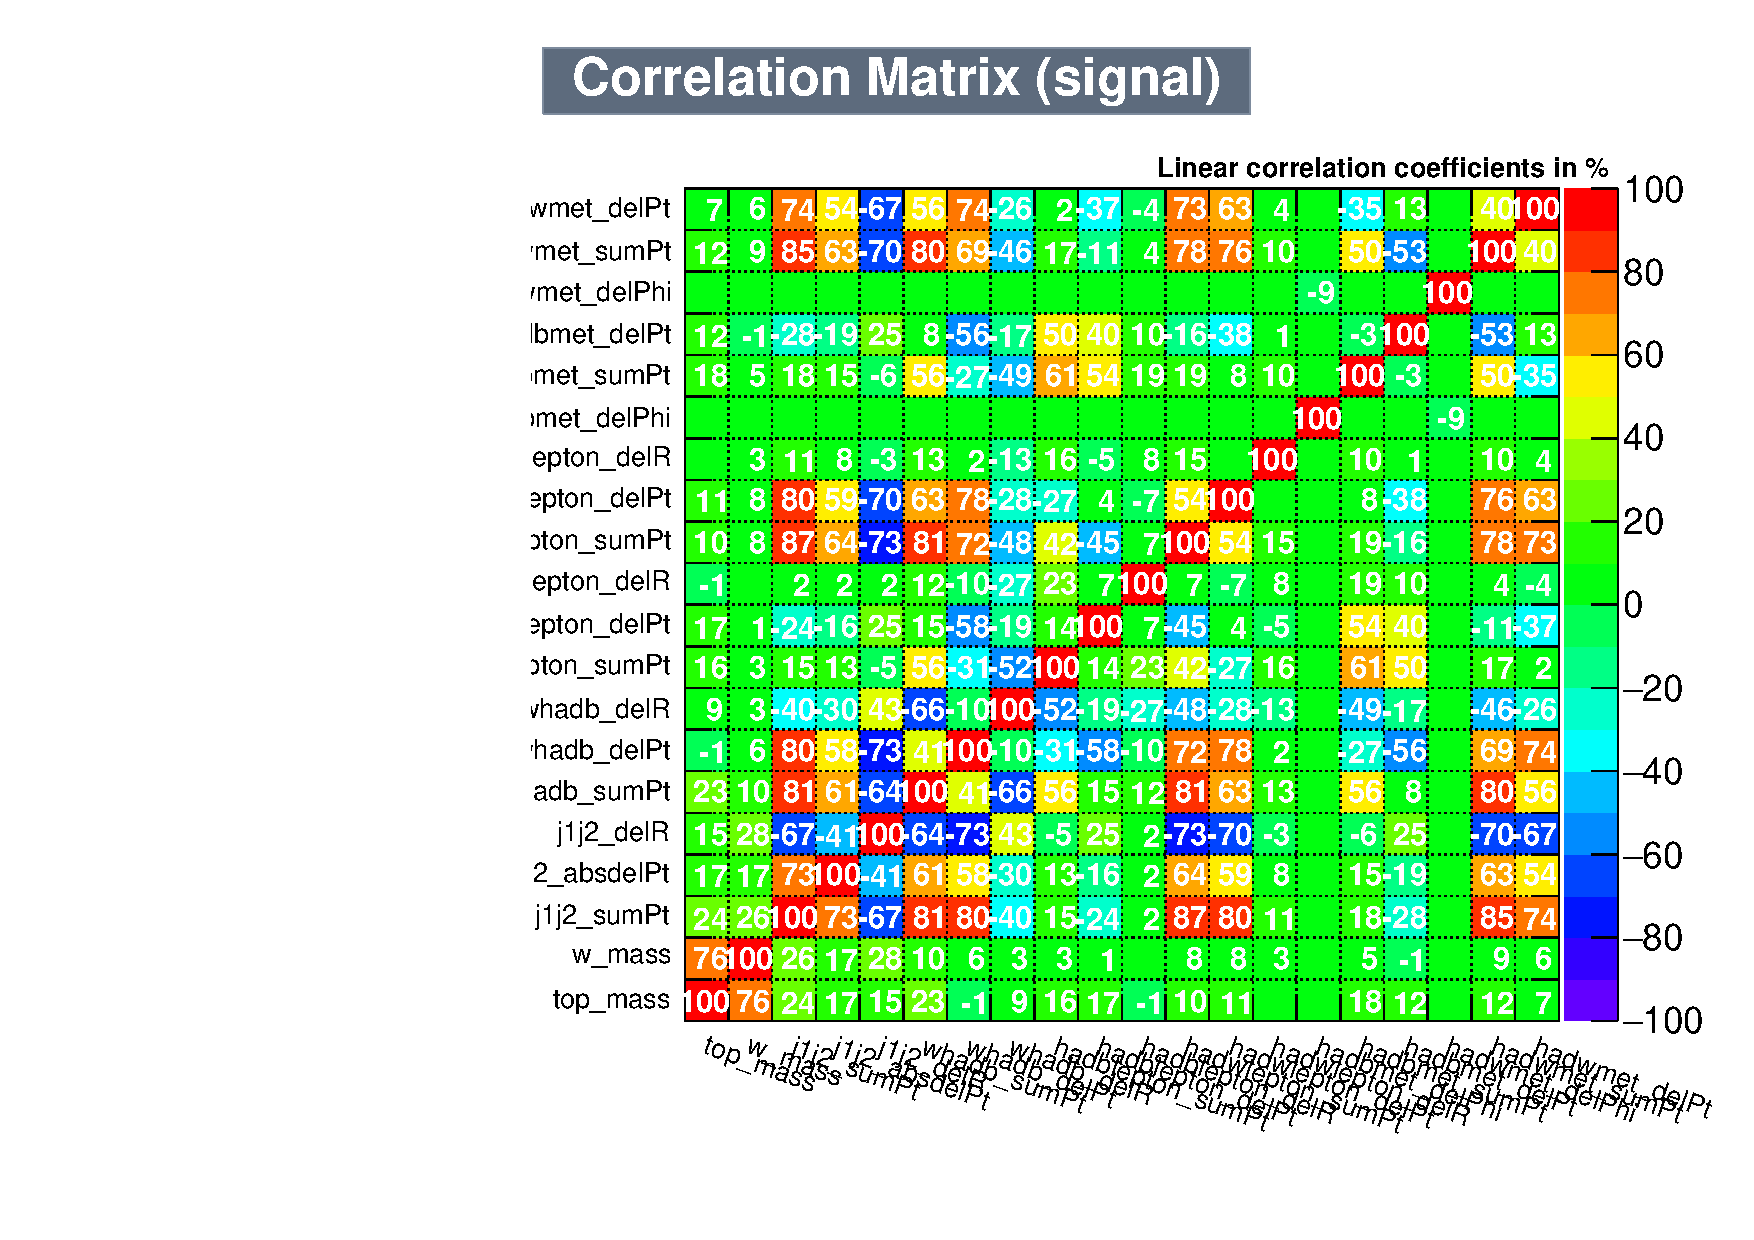
\includegraphics[width=0.45\textwidth]{Figures/EventSelReco/mva/a05_sig_cor.pdf}}
			    \subfigure[Variables in background]{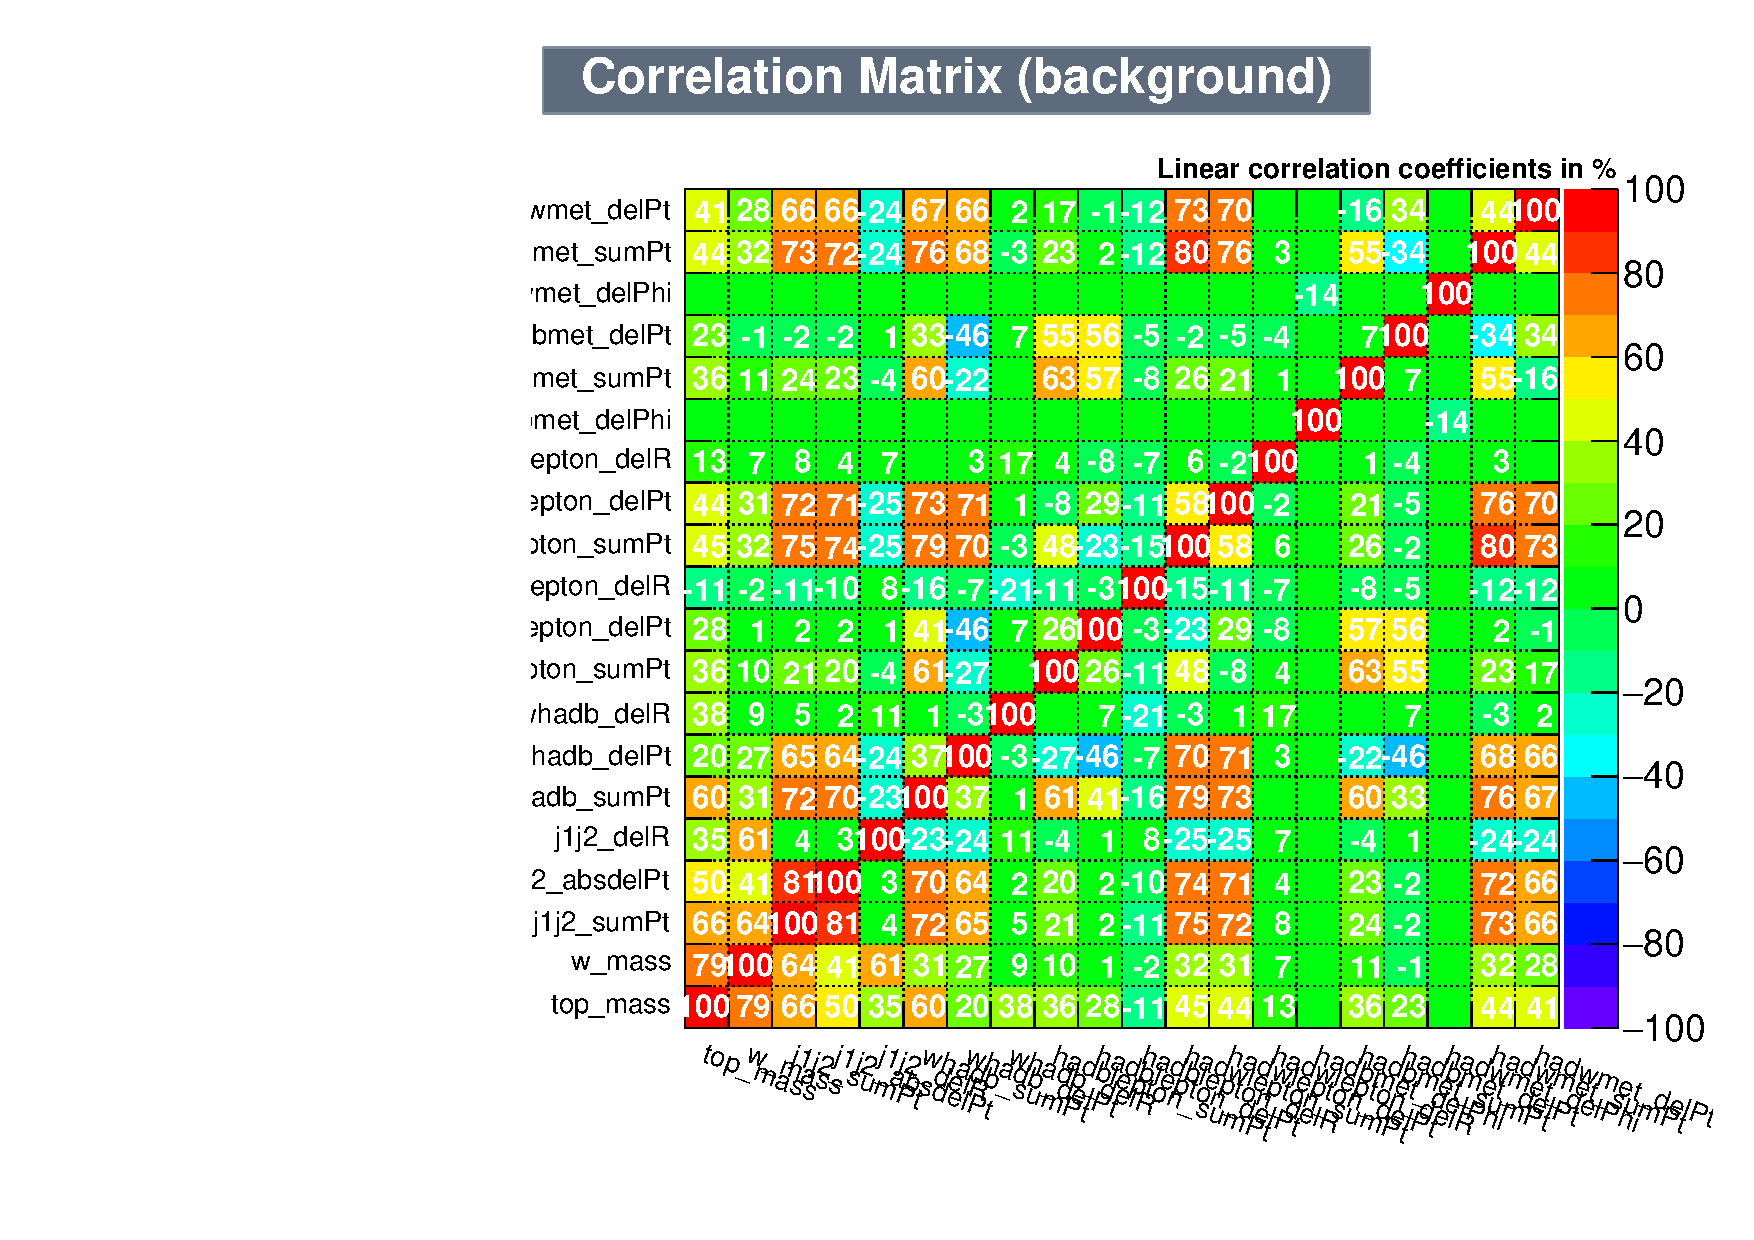
\includegraphics[width=0.45\textwidth]{Figures/EventSelReco/mva/a05_bkg_cor.pdf}}\\
			\caption{Variables correlation with each other}
			\label{EventSelReco:fig:a05_correlation}
			\end{figure}
			\FloatBarrier

			No excess of correlation appear in training variables. The training variables would be also validated match between Data and MC:(20 variables MLP, muon channel is shown)

			\begin{figure}[H]
			\centering
			    \subfigure{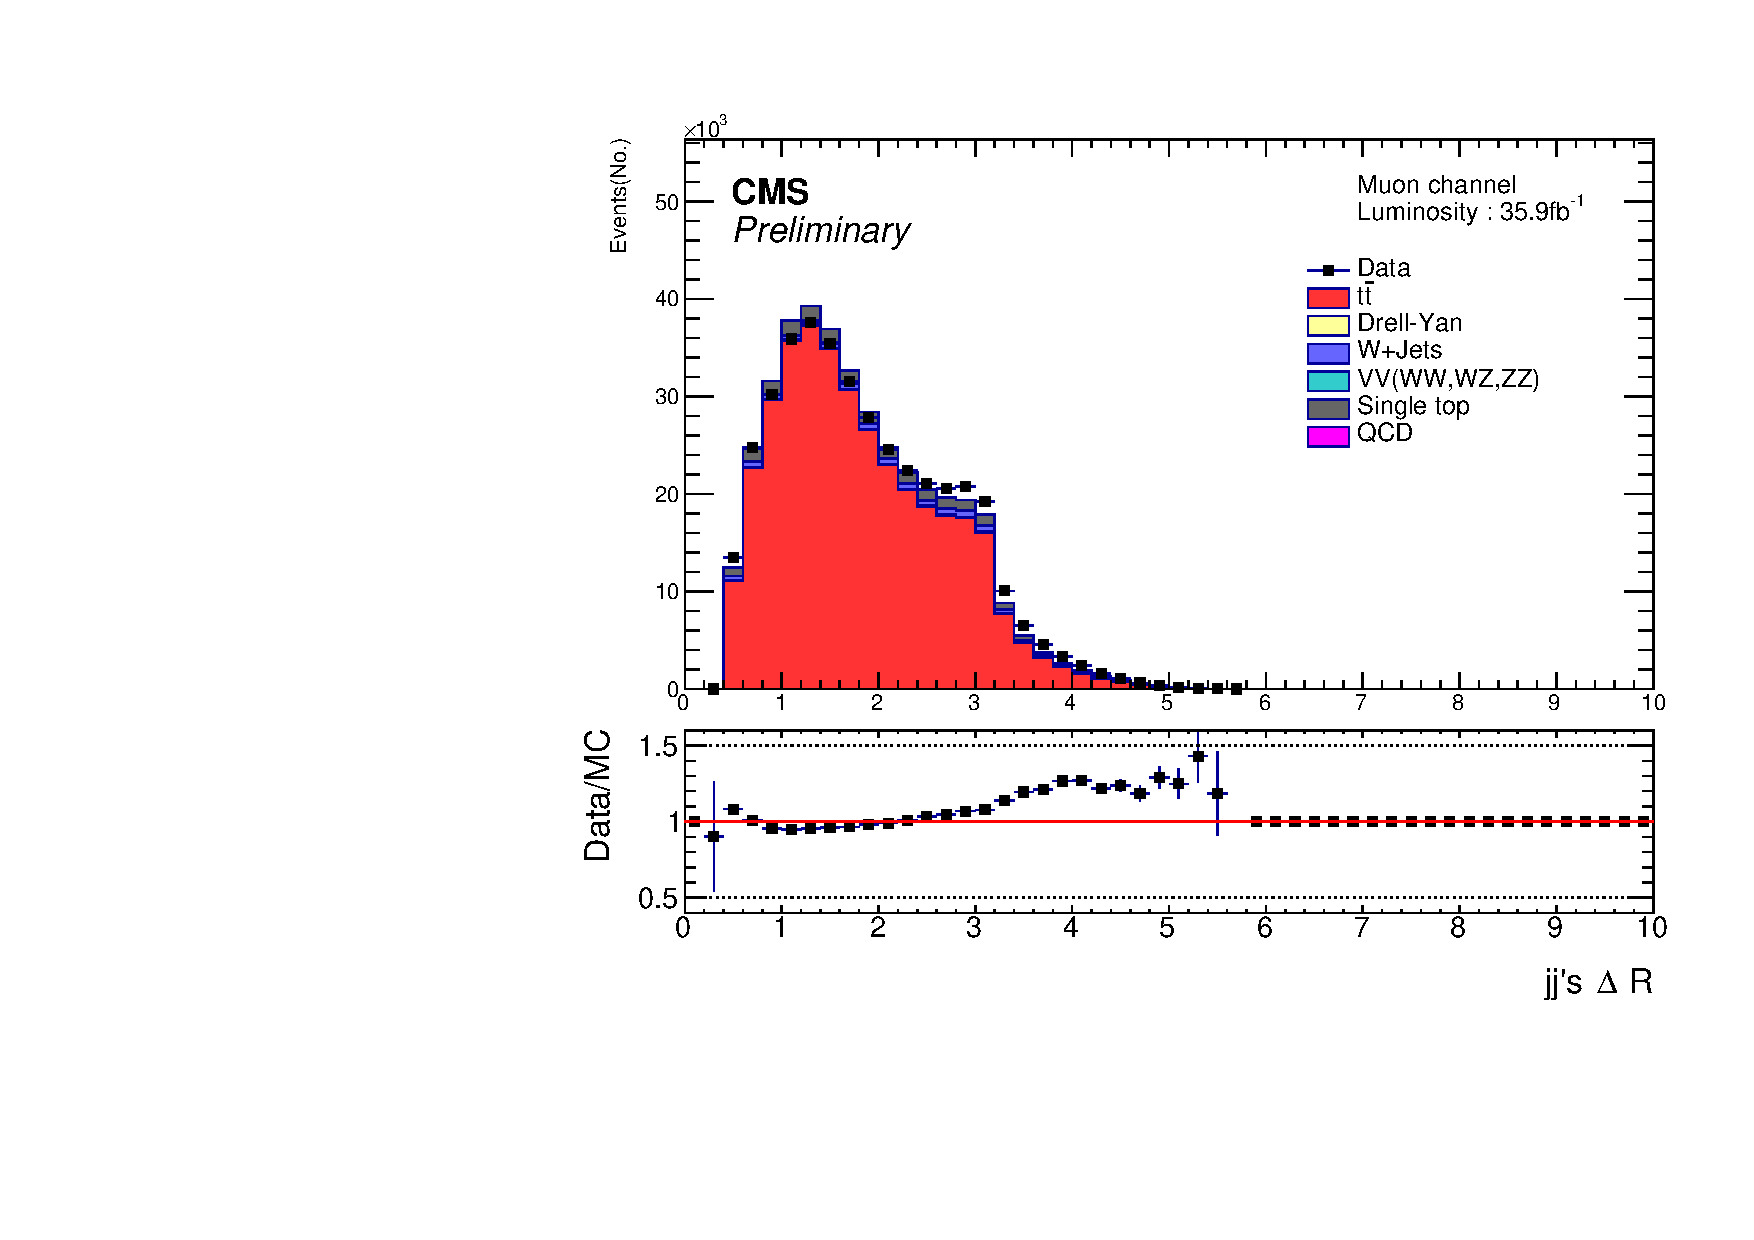
\includegraphics[width=0.32\textwidth]{Figures/EventSelReco/mva_vars/VarCheck_j1j2_delR_NC_mu.pdf}}
			    \subfigure{\includegraphics[width=0.32\textwidth]{Figures/EventSelReco/mva_vars/VarCheck_j1j2_absdelPt_NC_mu.pdf}}
			    \subfigure{\includegraphics[width=0.32\textwidth]{Figures/EventSelReco/mva_vars/VarCheck_j1j2_sumPt_NC_mu.pdf}}\\
			\end{figure}
			\FloatBarrier

			\begin{figure}[H]
			\centering
			    \subfigure{\includegraphics[width=0.32\textwidth]{Figures/EventSelReco/mva_vars/VarCheck_whadb_delR_NC_mu.pdf}}
			    \subfigure{\includegraphics[width=0.32\textwidth]{Figures/EventSelReco/mva_vars/VarCheck_whadb_delPt_NC_mu.pdf}}
			    \subfigure{\includegraphics[width=0.32\textwidth]{Figures/EventSelReco/mva_vars/VarCheck_whadb_sumPt_NC_mu.pdf}}\\
			\end{figure}
			\FloatBarrier

			\begin{figure}[H]
			\centering
			    \subfigure{\includegraphics[width=0.32\textwidth]{Figures/EventSelReco/mva_vars/VarCheck_hadblepton_delR_NC_mu.pdf}}
			    \subfigure{\includegraphics[width=0.32\textwidth]{Figures/EventSelReco/mva_vars/VarCheck_hadblepton_delPt_NC_mu.pdf}}
			    \subfigure{\includegraphics[width=0.32\textwidth]{Figures/EventSelReco/mva_vars/VarCheck_hadblepton_sumPt_NC_mu.pdf}}\\
			\end{figure}
			\FloatBarrier

			\begin{figure}[H]
			\centering
			    \subfigure{\includegraphics[width=0.32\textwidth]{Figures/EventSelReco/mva_vars/VarCheck_hadwlepton_delR_NC_mu.pdf}}
			    \subfigure{\includegraphics[width=0.32\textwidth]{Figures/EventSelReco/mva_vars/VarCheck_hadwlepton_delPt_NC_mu.pdf}}
			    \subfigure{\includegraphics[width=0.32\textwidth]{Figures/EventSelReco/mva_vars/VarCheck_hadwlepton_sumPt_NC_mu.pdf}}\\
			\end{figure}
			\FloatBarrier

			\begin{figure}[H]
			\centering
			    \subfigure{\includegraphics[width=0.32\textwidth]{Figures/EventSelReco/mva_vars/VarCheck_hadwmet_delPhi_NC_mu.pdf}}
			    \subfigure{\includegraphics[width=0.32\textwidth]{Figures/EventSelReco/mva_vars/VarCheck_hadwmet_delPt_NC_mu.pdf}}
			    \subfigure{\includegraphics[width=0.32\textwidth]{Figures/EventSelReco/mva_vars/VarCheck_hadwmet_sumPt_NC_mu.pdf}}\\
			\end{figure}
			\FloatBarrier

			\begin{figure}[H]
			\centering
			    \subfigure{\includegraphics[width=0.32\textwidth]{Figures/EventSelReco/mva_vars/VarCheck_hadbmet_delPhi_NC_mu.pdf}}
			    \subfigure{\includegraphics[width=0.32\textwidth]{Figures/EventSelReco/mva_vars/VarCheck_hadbmet_delPt_NC_mu.pdf}}
			    \subfigure{\includegraphics[width=0.32\textwidth]{Figures/EventSelReco/mva_vars/VarCheck_hadbmet_sumPt_NC_mu.pdf}}\\
			\end{figure}
			\FloatBarrier

			\begin{figure}[H]
			\centering
			    \subfigure{\includegraphics[width=0.45\textwidth]{Figures/EventSelReco/mva_vars/VarCheck_mjj_NC_mu.pdf}}
			    \subfigure{\includegraphics[width=0.45\textwidth]{Figures/EventSelReco/Mass/a05/a05_MLP_NC_long_HadTop_mu.pdf}}\\
			\label{EventSelReco:fig:a05_DataMC_vars}
			\caption{20 variables' Data/MC comparison(MLP, mu-ch)}
			\end{figure}
			\FloatBarrier

	\subsection{$b\bar{b}$ separation and distinguishment}
	\label{ssec:bbsep}

		The good correctness of chosen physical objects is necessary in this analysis. By the basis for discovering new physics, the observables require precise identification of particles. And the important is, in our selected observables, to distinguish $b$- between $\bar{b}$ -quark which are both b-tagged jets detected from smashing and hadronizatoin of b-flavor quarks. For example, the identification is highly correlated with observable $O_{6}$ which is $q_{l}(\vec{p_{b}}-\vec{p_{\bar{b}}})\cdot(\vec{p_{l}}\times\vec{p_{j_{1}}})$, the mis-ordered $b$/($\bar{b}$) will cause the wrong sign on this observable. On the other hand, it is not requirement for us to correctly pick up the 2 jets from hadronic top quark in this analysis. Also, the long tail in reconstructed hadronic top invariant mass($M_{jjb}$, Fig.\ref{EventSelReco:fig:a04_MLP_SR_NC_Mjjb}, Fig.\ref{EventSelReco:fig:t13_MLP_SR_NC_Mjjb}, Fig.\ref{EventSelReco:fig:a05_MLP_SR_NC_Mjjb}) deviated too much from known top mass 172.5GeV. And the source of this tail is infered coming from $b/\bar{b}$ wrong identified cases. In this way, the identification between $b$ and $\bar{b}$ is the most critical implication. And that is also what we need to test the performance of reconstruction algorithm($\chi^2_{min}$,MVA). 

		All the following study in \ref{ssec:bbsep} is worked only under the signal simulation sample($t$$\bar{t}$ Monte Carlo). All the selected physical objects include jets and leptons will be matched to particle with the generator-level information in MC sample with $\Delta R$ < 0.4 method.(Eq.\ref{eq:gen_matching})

		To standardlize the $b$/$\bar{b}$ distinguishment, there are 3 classifications listed:
		\begin{itemize}
  		\item $\textbf{Correct}$: $b$-quark is identified as $b$-jets and $\bar{b}$-quark is identified as $\bar{b}$-jets
  		\item $\textbf{b/}$$\bar{\textbf{b}}$ $\textbf{mis-identified}$: $b$-quark is identified as $\bar{b}$-jets and $\bar{b}$-quark is identified as $b$-jets
  		\item $\textbf{Mistag}$: non $b$$(\bar{b})$-quark is identified as $b$$(\bar{b})$-jet
		\end{itemize}

		With applying the various algorithm on signal simulation sample($t\bar{t}$ MC), there are the $b/\bar{b}$-distinguishment results after reconstructed the hadronic top and make a identification of physical objects via $\chi^2_{min}$ and MVA methods:

		\begin{center}
		\begin{longtable}[H]{ c c | c c c }			% add the [H] can make it listed in table list!!
		\caption{$b/\bar{b}$ disdinguishment under different algorithm (w/o cut)}\\
		\hline
		[\%] & & Correct & $b\bar{b}$ mis-identified & Mistag  \\ 
		\hline
		$\chi^2_{min}$ &  &    61.18 & 25.21 & 13.38 \\
		\hline
		\multirow{3}{5em}{2 variables} & MLP & 63.18 & 23.22 & 13.60 \\
		& BDT & 60.89 & 25.49 & 13.60 \\
		& BDTG & 63.02 & 23.37 & 13.61 \\
		\hline
		\multirow{3}{5em}{8 variables} & MLP & 72.36 & 14.02 & 13.62 \\
		& BDT & 72.02 & 14.37 & 13.60 \\
		& BDTG & 71.00 & 15.39 & 13.61 \\
		\hline
		\multirow{3}{5em}{20 variables} & MLP & 71.27 & 15.13 & 13.61 \\
		& BDT & 71.07 & 15.32 & 13.61 \\
		& BDTG & 69.59 & 16.79 & 13.61 \\
		\hline
		\label{EventSelReco:tb:nocut_bbsep}
		\end{longtable}
		\end{center}

		This is shown that the MLP algorithm have the best performance under these 3 training variables sets. As our expected, the 2 variables training result is close to $\chi^2_{min}$ method's because of their same variables input to be deduced. And the 8 variables set and 20 variables set are both good at discreminate $b/\bar{b}$, which can lead us to choose these to be optimized one. It is also known that $\emph{Mistag}$'s ratio in Table.\ref{EventSelReco:tb:nocut_bbsep} are almost the same since it is primarily pre-decided by the b-tagged selection.

		In addition to applying algorithm to reconstruct $M_{jjb}$ and identify the physical objects, there are also some optimization cut done on this step. In the concept of $\chi^2_{min}$ method, the smaller the $\chi^2$ value(Eq.\ref{eq:chi2}), the less possibility that this combination is the one we want. So we can apply cut on $\chi^2$ value. If in an event the chosen combination whose $\chi^2_{min}$ is still bigger than the cut, the event will be threw away. These thrown away events are identified as the events which come from the mis-tag objects from detector or some events come from other physics decay(background) not $t\bar{t}$. The most important is that, it can cut out the events which are not $b/\bar{b}$-correct distinguished. So the cut is set to be at $\chi^2_{min}$ < 20, and to standardize the optimization, there are also use the $b/\bar{b}$ distinguishment results to see the performance.

		There is the cross-check plot(Fig.\ref{EventSelReco:fig:chi2_2D}) which shows that the high $\chi^2$ value correspond to the $m_{jjb}$ distant from the expected $m_{jjb}$ in Eq.\ref{eq:chi2}.

		\begin{figure}[H]
		\centering{}
    		\includegraphics[width=0.65\textwidth]{Figures/EventSelReco/bbsep/chi2_2D.pdf}\\
		\caption{$\chi^2_{min}$-reco $m_{jjb}$}
		\label{EventSelReco:fig:chi2_2D}
		\end{figure}
		\FloatBarrier

		To check that the cut on the $\chi^2_{min}$ really rule out incorrect $b/\bar{b}$-identified more effeciently than correct case. This plot(Fig.\ref{EventSelReco:fig:chi2_bbsep_pdf}) shows that the incorrect cases(exchange-identified and mistag) do have more ratio at the higher $\chi^2_{min}$ score than the correct case. It make the $\chi^2_{min}$ cut more persuasive.

		\begin{figure}[H]
		\centering
		    \includegraphics[width=0.65\textwidth]{Figures/EventSelReco/bbsep/chi2_bbsep.pdf}\\
		\caption{$b/\bar{b}$ identified result related to $\chi^2_{min}$(pdf)}
		\label{EventSelReco:fig:chi2_bbsep_pdf}
		\end{figure}
		\FloatBarrier

		There is the result that if we cut on the $\chi^2_{min}$ value and how the 3 $b/\bar{b}$-identified classifications' ratios vary. It is also shown that the events efficiency which is the ratio of events survived under this optimized cut.

		\begin{figure}[H]
		\centering
		    \includegraphics[width=0.65\textwidth]{Figures/EventSelReco/bbsep/chi2_eff_t.pdf}\\ 
		\caption{cut on $\chi^2_{min}$ and ratio of 3 classification}
		\label{EventSelReco:fig:chi2_bbsep_eff}
		\end{figure}
		\FloatBarrier

		\begin{center}
		\begin{longtable}[H]{ c c | c c c }
		\caption{$b/\bar{b}$ disdinguishment under $\chi^2_{min}$ method (w/ $\chi^2_{min}$ < 20 cut)}\\
		\hline
		[\%] & Channel & Correct & $b\bar{b}$ mis-identified & Mistag  \\ 
		\hline{}
		\multirow{2}{2em}{$\chi^2_{min}$} & Electron Channel & 65.47 & 22.29 & 12.24 \\
		& Muon Channel & 65.65 & 22.29 & 12.06 \\
		\hline
		\label{EventSelReco:tb:chi2_algocut_bbsep}
		\end{longtable}
		\end{center}

		And as same concept as the optimized cut on $\chi^2_{min}$ value in $\chi^2_{min}$ method, there would be also optimization cut applied on MVA method. In comparison with that low $\chi^2$ value is better choice, combination with high MVA score is the better one in MVA method. It also can have a cut on MVA score to subtract incorrect $b/\bar{b}$-identified selection. Same scenario as $\chi^2_{min}$ method, if in an event the maximum MVA score(which belongs to the chosen combination) is still lower than the cut, the event will be threw away. We still need to check the relation between MVA score and $M_{jjb}$, and also check the ratio of 3 $b/\bar{b}$-classifications that the incorrect cases has more ratio at lower MVA score. There are the plots of 2 variables/8 variables/20 variables sets with MLP/BDT/BDTG training method:

		\begin{figure}[H]
		\centering
			\subfigure[BDT]{\includegraphics[width=0.32\textwidth]{Figures/EventSelReco/bbsep/a04_BDT_2D.pdf}}
			\subfigure[BDTG]{\includegraphics[width=0.32\textwidth]{Figures/EventSelReco/bbsep/a04_BDTG_2D.pdf}}
			\subfigure[MLP]{\includegraphics[width=0.32\textwidth]{Figures/EventSelReco/bbsep/a04_MLP_2D.pdf}}\\
			\subfigure[BDT]{\includegraphics[width=0.32\textwidth]{Figures/EventSelReco/bbsep/a04_BDT_bbsep3.pdf}}
			\subfigure[BDTG]{\includegraphics[width=0.32\textwidth]{Figures/EventSelReco/bbsep/a04_BDTG_bbsep3.pdf}}
		    \subfigure[MLP]{\includegraphics[width=0.32\textwidth]{Figures/EventSelReco/bbsep/a04_MLP_bbsep3.pdf}}\\
		\caption{MVA score-reco $m_{jjb}$ plots and $b/\bar{b}$ identified result related to MVA value (2 variables training)}
		\label{EventSelReco:fig:a04_bbsep}
		\end{figure}
		\FloatBarrier

		\begin{figure}[H]
		\centering
			\subfigure[BDT]{\includegraphics[width=0.32\textwidth]{Figures/EventSelReco/bbsep/t13_BDT_2D.pdf}}
			\subfigure[BDTG]{\includegraphics[width=0.32\textwidth]{Figures/EventSelReco/bbsep/t13_BDTG_2D.pdf}}
			\subfigure[MLP]{\includegraphics[width=0.32\textwidth]{Figures/EventSelReco/bbsep/t13_MLP_2D.pdf}}\\
			\subfigure[BDT]{\includegraphics[width=0.32\textwidth]{Figures/EventSelReco/bbsep/t13_BDT_bbsep3.pdf}}
			\subfigure[BDTG]{\includegraphics[width=0.32\textwidth]{Figures/EventSelReco/bbsep/t13_BDTG_bbsep3.pdf}}
		    \subfigure[MLP]{\includegraphics[width=0.32\textwidth]{Figures/EventSelReco/bbsep/t13_MLP_bbsep3.pdf}}\\
		\caption{MVA score-reco $m_{jjb}$ plots and $b/\bar{b}$ identified result related to MVA value (8 variables training)}
		\label{EventSelReco:fig:t13_bbsep}
		\end{figure}
		\FloatBarrier

		\begin{figure}[H]
		\centering
			\subfigure[BDT]{\includegraphics[width=0.32\textwidth]{Figures/EventSelReco/bbsep/a05_BDT_2D.pdf}}
			\subfigure[BDTG]{\includegraphics[width=0.32\textwidth]{Figures/EventSelReco/bbsep/a05_BDTG_2D.pdf}}
			\subfigure[MLP]{\includegraphics[width=0.32\textwidth]{Figures/EventSelReco/bbsep/a05_MLP_2D.pdf}}\\
			\subfigure[BDT]{\includegraphics[width=0.32\textwidth]{Figures/EventSelReco/bbsep/a05_BDT_bbsep3.pdf}}
			\subfigure[BDTG]{\includegraphics[width=0.32\textwidth]{Figures/EventSelReco/bbsep/a05_BDTG_bbsep3.pdf}}			
		    \subfigure[MLP]{\includegraphics[width=0.32\textwidth]{Figures/EventSelReco/bbsep/a05_MLP_bbsep3.pdf}}\\
		\caption{MVA score-reco $m_{jjb}$ plots and $b/\bar{b}$ identified result related to MVA value (20 variables training)}
		\label{EventSelReco:fig:a05_bbsep}
		\end{figure}
		\FloatBarrier

		There are also the effeciency plots shows that if it's given a cut on MVA score, how these 3 $b/\bar{b}$-identified cases' ratio vary.

		\begin{figure}[H]
		\centering
			\subfigure[BDT]{\includegraphics[width=0.32\textwidth]{Figures/EventSelReco/bbsep/a04_BDT_eff_t.pdf}}
			\subfigure[BDTG]{\includegraphics[width=0.32\textwidth]{Figures/EventSelReco/bbsep/a04_BDTG_eff_t.pdf}}
			\subfigure[MLP]{\includegraphics[width=0.32\textwidth]{Figures/EventSelReco/bbsep/a04_MLP_eff_t.pdf}}\\
		\caption{cut on MVA score and ratio of 3 classification (2 variables training)}
		\label{EventSelReco:fig:a04_bbsep_eff}
		\end{figure}
		\FloatBarrier

		\begin{figure}[H]
		\centering
			\subfigure[BDT]{\includegraphics[width=0.32\textwidth]{Figures/EventSelReco/bbsep/t13_BDT_eff_t.pdf}}
			\subfigure[BDTG]{\includegraphics[width=0.32\textwidth]{Figures/EventSelReco/bbsep/t13_BDTG_eff_t.pdf}}
			\subfigure[MLP]{\includegraphics[width=0.32\textwidth]{Figures/EventSelReco/bbsep/t13_MLP_eff_t.pdf}}\\
		\caption{cut on MVA score and ratio of 3 classification (8 variables training)}
		\label{EventSelReco:fig:t13_bbsep_eff}
		\end{figure}
		\FloatBarrier

		\begin{figure}[H]
		\centering
			\subfigure[BDT]{\includegraphics[width=0.32\textwidth]{Figures/EventSelReco/bbsep/a05_BDT_eff_t.pdf}}
			\subfigure[BDTG]{\includegraphics[width=0.32\textwidth]{Figures/EventSelReco/bbsep/a05_BDTG_eff_t.pdf}}
			\subfigure[MLP]{\includegraphics[width=0.32\textwidth]{Figures/EventSelReco/bbsep/a05_MLP_eff_t.pdf}}\\
		\caption{cut on MVA score and ratio of 3 classification (20 variables training)}
		\label{EventSelReco:fig:a05_bbsep_eff}
		\end{figure}
		\FloatBarrier

		The correct ratio increase when the MVA score-cut is applied on higher value. Based on the target to optimized from $\chi^2_{min}$ method, we have cut on the same events efficiency as $\chi^2_{min}$ method when cutting on $\chi^2_{min}$ < 20, which is $\sim$$75\%$, to get the better ratio of correct-$b/\bar{b}$ case. There are the MVA-score cut at events efficiency $\sim$$75\%$:

		\begin{center}
		\begin{longtable}[H]{ c c c c c }
		\caption{MVA-score cut at events efficiency $\sim$75\%}\\
		\hline
		MVA score cut & BDT & BDTG & MLP(ANN)  \\ 
		\hline{}
		2 variables & -0.21 & -0.57 & 0.2 \\
		8 variables & -0.1 & -0.28 & 0.16 \\
		20 variables & -0.1 & -0.5 & 0.22 \\
		\hline
		\label{EventSelReco:tb:algocut_value}
		\end{longtable}
		\end{center}

		There are the $b/\bar{b}$-identified classifications' ratio after cut on events efficiency at $\sim 75\%$(cut value in Table.\ref{EventSelReco:tb:algocut_value}), test by signal simulation sample($t\bar{t}$ MC):

		\begin{center}
		\begin{longtable}[H]{ c c | c c c }
		\caption{$b/\bar{b}$ disdinguishment under different algorithm (w/ MVA cut)}\\
		\hline
		[\%] & & Correct & $b\bar{b}$ mis-identified & Mistag  \\ 
		\hline
		$\chi^2_{min}$ & & 65.58 & 22.33 & 12.09 \\
		\hline
		\multirow{3}{5em}{2 variables} & MLP & 69.22 & 19.43 & 11.35 \\
		& BDT & 68.26 & 20.95 & 10.79 \\
		& BDTG & 68.95 & 19.69 & 11.36 \\
		\hline
		\multirow{3}{5em}{8 variables} & MLP & 76.88 & 12.35 & 10.77 \\
		& BDT & 75.98 & 13.08 & 10.94 \\
		& BDTG & 75.37 & 13.68 & 10.95 \\
		\hline
		\multirow{3}{5em}{20 variables} & MLP & 76.41 & 12.34 & 11.25 \\
		& BDT & 75.13 & 13.20 & 11.67 \\
		& BDTG & 74.72 & 13.76 & 11.52 \\
		\hline
		\label{EventSelReco:tb:algocut_bbsep}
		\end{longtable}
		\end{center}

		Comparing Table.\ref{EventSelReco:tb:nocut_bbsep} to Table.\ref{EventSelReco:tb:algocut_bbsep}, it really make progress on the $b/\bar{b}$ separation with cut on algorithm value. 

		Besides the hadronic top's mass spectrum, there would be checked that the leptonic top's invariant mass($M_{lb}$) shows. Even though the missing neutrino's 4-momentum cause the leptonic top reconstructed incompletely, it's also valuable of $M_{lb}$ to be an independent information for other analysis strategy. Exactly, the $M_{lb}$ is the primary variable to be analyzed for the relation between signal/background and between data/simulation in this analysis! For instatnce, the following background estimation(Chapter.\ref{sec:BkgEst}).

		And for the $b/\bar{b}$ part, $b/\bar{b}$-identified types can also be shown under $M_{lb}$, they are also separated obviously with $\chi^2_{min}$ method:

		\begin{figure}[H]
		\centering
			\includegraphics[width=0.7\textwidth]{Figures/EventSelReco/bbsep/chi2_bbsep_leptop_t.pdf}
		\caption{The $M_{lb}$ and corresponding $b/\bar{b}$-separation under $\chi^2_{min}$ method.}
		\label{EventSelReco:fig:chi2_bbsep_leptop}
		\end{figure}
		\FloatBarrier

		It's decide to cut on $M_{lb}$ = 150 GeV and leave the events below the value. It can effectively eliminate the high ratio of events whose decay objects are wrong-identified. And follow the same reason as $\chi^2_{min}$ method, the MVA methods are also check with $M_{lb}$ spectrum:

		\begin{figure}[H]
		\centering
			\subfigure[BDT]{\includegraphics[width=0.32\textwidth]{Figures/EventSelReco/bbsep/a04_BDT_bbsep_leptop_t.pdf}}
			\subfigure[BDTG]{\includegraphics[width=0.32\textwidth]{Figures/EventSelReco/bbsep/a04_BDTG_bbsep_leptop_t.pdf}}
			\subfigure[MLP]{\includegraphics[width=0.32\textwidth]{Figures/EventSelReco/bbsep/a04_MLP_bbsep_leptop_t.pdf}}\\
		\caption{Relation between $M_{lb}$ and $b/\bar{b}$ with MVA reconstruction result.(2 variables)}
		\label{EventSelReco:fig:a05_bbsep_eff}
		\end{figure}
		\FloatBarrier

		\begin{figure}[H]
		\centering
			\subfigure[BDT]{\includegraphics[width=0.32\textwidth]{Figures/EventSelReco/bbsep/t13_BDT_bbsep_leptop_t.pdf}}
			\subfigure[BDTG]{\includegraphics[width=0.32\textwidth]{Figures/EventSelReco/bbsep/t13_BDTG_bbsep_leptop_t.pdf}}
			\subfigure[MLP]{\includegraphics[width=0.32\textwidth]{Figures/EventSelReco/bbsep/t13_MLP_bbsep_leptop_t.pdf}}\\
		\caption{Relation between $M_{lb}$ and $b/\bar{b}$ with MVA reconstruction result.(8 variables)}
		\label{EventSelReco:fig:a05_bbsep_eff}
		\end{figure}
		\FloatBarrier

		\begin{figure}[H]
		\centering
			\subfigure[BDT]{\includegraphics[width=0.32\textwidth]{Figures/EventSelReco/bbsep/a05_BDT_bbsep_leptop_t.pdf}}
			\subfigure[BDTG]{\includegraphics[width=0.32\textwidth]{Figures/EventSelReco/bbsep/a05_BDTG_bbsep_leptop_t.pdf}}
			\subfigure[MLP]{\includegraphics[width=0.32\textwidth]{Figures/EventSelReco/bbsep/a05_MLP_bbsep_leptop_t.pdf}}\\
		\caption{Relation between $M_{lb}$ and $b/\bar{b}$ with MVA reconstruction result.(20 variables)}
		\label{EventSelReco:fig:a05_bbsep_eff}
		\end{figure}
		\FloatBarrier

		In 8 variables and 20 variables cases, the $M_{lb}$ looks not to be separated by $b/\bar{b}$-identification obviously, that is, it may not improve when applying $M_{lb}$ cut at 150 GeV. However, there are the $b/\bar{b}$-identified ratio after MVA(or $\chi^2$) cut and $M_{lb}$ cut.

		%% show the bbsep ratio after leptop cut 

		\begin{center}
		\begin{longtable}[H]{ c c | c c c | c }
		\caption{$b/\bar{b}$ disdinguishment under different algorithm (w/ MVA cut and $M_{lb}$ cut)}\\
		\hline
		[\%] & & Correct & $b\bar{b}$ mis-identified & Mistag & Events efficiency  \\ 
		\hline
		$\chi^2_{min}$ & & 75.56 & 14.70 & 9.74 & 65.39 \\
		\hline
		\multirow{3}{5em}{2 variables} & MLP & 78.03 & 12.92 & 9.00 & 64.84  \\
		& BDT & 77.66 & 13.69 & 8.65 & 64.92 \\
		& BDTG & 77.91 & 13.01 & 9.08 & 64.57  \\
		\hline
		\multirow{3}{5em}{8 variables} & MLP & 78.77 & 11.50 & 9.73 & 71.55 \\
		& BDT & 78.12 & 12.05 & 9.83 & 71.44 \\
		& BDTG & 77.05 & 12.94 & 10.01 & 71.29 \\
		\hline
		\multirow{3}{5em}{20 variables} & MLP & 80.51 & 10.24 & 9.25 & 69.26 \\
		& BDT & 79.34 & 11.01 & 9.65 & 69.09 \\
		& BDTG & 78.67 & 11.76 & 9.57 & 69.99 \\
		\hline{}
		\label{EventSelReco:tb:algocut_mlbcut_bbsep}
		\end{longtable}
		\end{center}
		\FloatBarrier

		\begin{itemize}
			\item Final $\chi^2_{min}$ strategy is decided to be with $\chi^2_{min}$ value cut at 20 and $M_{lb}$ cut at 150GeV.\\
			It is called $\chi^{\textbf{2}}_{\textbf{min}}$ $\textbf{strategy}$ in the following content.
		\end{itemize}
		The improvement is still shown with $M_{lb}$ cut in all MVA method by comparing Table.\ref{EventSelReco:tb:algocut_bbsep} and Table.\ref{EventSelReco:tb:algocut_mlbcut_bbsep}. The MLP is the most suitable algorithm after these test. The 8 variables case will be eliminated for the reason explained at Fig.\ref{EventSelReco:fig:CR_shape_MVAcut} in \ref{ssec:CR}, so the finally decided method which is the most optimized is 20 variables treaining with MLP algorithm. There are 2 choice of analysis strategy with this 20 variables MLP training result: 

		\begin{enumerate}
			\item $\textbf{The first}$ is with MVA(MLP) cut at 0.22 (events efficiency $\sim 75\%$) and also cut on $M_{lb}$ at 150GeV.\\ 
			The correct $b/\bar{b}$ ratio is $\sim 5 \%$($80.51 \%/75.56 \%$) better and the events efficiency is $\sim 4 \%$($69.26 \%/65.39 \%$) more than $\chi^2_{min}$ strategy.\\
			This MVA result would be called $\textbf{MVA-A}$ $\textbf{strategy}$ in the following content;
			\item $\textbf{The second}$ is only with MVA(MLP) cut at 0.22 but $M_{lb}$ cut. \\
			Though the correct $b/\bar{b}$ ratio is just $\sim 1 \%$($76.88 \%/75.56 \%$) better, the events efficiency would be reserve $\sim 9.5 \%$($74.97 \%/65.39 \%$) more than $\chi^2_{min}$ strategy. The advantage of this is that the more statistics we retain, the precise the calculation of asymmetry eventually because the statistical and systematic uncertainty would be smaller.\\
			This MVA result would be called $\textbf{MVA-B}$ $\textbf{strategy}$ in the following content.
		\label{EventSelReco:itm:a05_samples}
		\end{enumerate}

		%% show the final sample ratio after full-cut (chi2, a05_MLP) and their mjjb plots

		There are the data events number passed full-selection(\ref{EventSelReco:itm:full_sel}) also with $\chi^{\textbf{2}}_{\textbf{min}}$ $\textbf{strategy}$ and the expected signal($t\bar{t}$) and background events number of simulation sample in Table.\ref{EventSelReco:tb:DataMC_expected_chi2}. The Table.\ref{EventSelReco:tb:MC_process_chi2} present the expected process ratio after full-selection cut and analysis strategy; The Data and MC comparison plots of hadronic top's invariant mass($M_{jjb}$) and leptonic top's invariant mass($M_{lb}$) are also shown(\r) with this criteria.

		\begin{center}
		\begin{longtable}[H]{ c c c }
		\caption{Data and MC events number passing the full selection(w/ $\chi^2_{min}, M_{lb}$ cut)} \\
		\hline
		 & Muon Channel & Electron Channel \\ 
		\hline
		 Data & 243790 & 136151 \\
		\hline
		 Expected $t\bar{t}$ & 244680 & 135600 \\
		 Expected background & 9877.63 & 5537.45 \\
		\hline
		\label{EventSelReco:tb:DataMC_expected_chi2}
		\end{longtable}
		\end{center}
		\FloatBarrier

		\begin{center}
		\begin{longtable}[H]{ c c c }
		\caption{Expected process ratio passing the full selection(w/ $\chi^2_{min}, M_{lb}$ cut)}\\
		\hline
		 Process & Muon Channel (\%) & Electron Channel (\%) \\ 
		\hline
		 $t\bar{t}+jets$ & 96.12 & 96.08 \\
		 $Z/\gamma^{*}+jets$ & 0.17 &  0.31 \\
		 $W+jets$ & 0.77 & 0.70 \\
		 $ZZ/WW/WZ$ & 0.04 & 0.05 \\
		 $Single$ $top$ & 2.91 & 2.86 \\
		\hline
		\label{EventSelReco:tb:MC_process_chi2}
		\end{longtable}
		\end{center}
		\FloatBarrier

		\begin{figure}[H]
		\centering
			\subfigure[Muon Channel]{\includegraphics[width=0.45\textwidth]{Figures/EventSelReco/Mass/chi2/200803_SRmass_chi2_2C_HadTop_mu.pdf}}
			\subfigure[Electron Channe]{\includegraphics[width=0.45\textwidth]{Figures/EventSelReco/Mass/chi2/200803_SRmass_chi2_2C_HadTop_el.pdf}}\\
		\caption{Data and MC comparison plots of hadronic top's invariant mass($M_{jjb}$ w/ $\chi^2_{min}, M_{lb}$ cut)}
		\label{EventSelReco:fig:chi2_SR_2C_Mjjb}
		\end{figure}
		\FloatBarrier

		\begin{figure}[H]
		\centering
			\subfigure[Muon Channel]{\includegraphics[width=0.45\textwidth]{Figures/EventSelReco/Mass/chi2/200803_SRmass_chi2_2C_LepTop_mu.pdf}}
			\subfigure[Electron Channel]{\includegraphics[width=0.45\textwidth]{Figures/EventSelReco/Mass/chi2/200803_SRmass_chi2_2C_LepTop_el.pdf}}\\
		\caption{Data and MC comparison plots of leptonic top's invariant mass($M_{lb}$ w/ $\chi^2_{min}, M_{lb}$ cut)}
		\label{EventSelReco:fig:chi2_SR_2C_Mlb}
		\end{figure}
		\FloatBarrier

		There are also the full selection results with $\textbf{MVA-A strategy}$(Table.\ref{EventSelReco:tb:DataMC_expected_a05_MLP_2C}, Table.\ref{EventSelReco:tb:MC_process_a05_MLP_2C}, Fig.\ref{EventSelReco:fig:a05_MLP_SR_2C_Mjjb}, Fig.\ref{EventSelReco:fig:a05_MLP_SR_2C_Mlb}) and $\textbf{MVA-B strategy}$(Table.\ref{EventSelReco:tb:DataMC_expected_a05_MLP_1C}, Table.\ref{EventSelReco:tb:MC_process_a05_MLP_1C}, Fig.\ref{EventSelReco:fig:a05_MLP_SR_1C_Mjjb}, Fig.\ref{EventSelReco:fig:a05_MLP_SR_1C_Mlb}):

		\begin{center}
		\begin{longtable}[H]{ c c c }
		\caption{Data and MC events number passing the full selection in SR(w/ MVA, $M_{lb}$ cut)} \\
		\hline
		 & Muon Channel & Electron Channel \\ 
		\hline
		 Data & 245436 & 139432 \\
		\hline
		 Expected $t\bar{t}$ & 251862 & 142211 \\
		 Expected background & 9164.09 & 5238.32 \\
		\hline
		\label{EventSelReco:tb:DataMC_expected_a05_MLP_2C}
		\end{longtable}
		\end{center}
		\FloatBarrier

		\begin{center}
		\begin{longtable}[H]{ c c c }
		\caption{Expected process ratio passing the full selection in SR(w/ MVA, $M_{lb}$ cut)}\\
		\hline
		 Process & Muon Channel (\%) & Electron Channel (\%) \\ 
		\hline
		 $t\bar{t}+jets$ & 96.49 & 96.45 \\
		 $Z/\gamma^{*}+jets$ & 0.14 &  0.26 \\
		 $W+jets$ & 0.67 & 0.62 \\
		 $ZZ/WW/WZ$ & 0.03 & 0.05 \\
		 $Single$ $top$ & 2.67 & 2.64 \\
		\hline
		\label{EventSelReco:tb:MC_process_a05_MLP_2C}
		\end{longtable}
		\end{center}
		\FloatBarrier

		\begin{figure}[H]
		\centering
			\subfigure[Muon Channel]{\includegraphics[width=0.45\textwidth]{Figures/EventSelReco/Mass/a05/200803_SRmass_a05_MLP_2C_HadTop_mu.pdf}}
			\subfigure[Electron Channe]{\includegraphics[width=0.45\textwidth]{Figures/EventSelReco/Mass/a05/200803_SRmass_a05_MLP_2C_HadTop_el.pdf}}\\
		\caption{Data and MC comparison plots of hadronic top's invariant mass($M_{jjb}$ w/ MVA, $M_{lb}$ cut)}
		\label{EventSelReco:fig:a05_MLP_SR_2C_Mjjb}
		\end{figure}
		\FloatBarrier

		\begin{figure}[H]
		\centering
			\subfigure[Muon Channel]{\includegraphics[width=0.45\textwidth]{Figures/EventSelReco/Mass/a05/200803_SRmass_a05_MLP_2C_LepTop_mu.pdf}}
			\subfigure[Electron Channel]{\includegraphics[width=0.45\textwidth]{Figures/EventSelReco/Mass/a05/200803_SRmass_a05_MLP_2C_LepTop_el.pdf}}\\
		\caption{Data and MC comparison plots of leptonic top's invariant mass($M_{lb}$ w/ MVA, $M_{lb}$ cut)}
		\label{EventSelReco:fig:a05_MLP_SR_2C_Mlb}
		\end{figure}
		\FloatBarrier


		\begin{center}
		\begin{longtable}[H]{ c c c }
		\caption{Data and MC events number passing the full selection in SR(w/ MVA cut)} \\
		\hline
		 & Muon Channel & Electron Channel \\ 
		\hline
		 Data & 272583 & 157510 \\
		\hline
		 Expected $t\bar{t}$ & 273154 & 155766 \\
		 Expected background & 14715.9 & 8957.06 \\
		\hline
		\label{EventSelReco:tb:DataMC_expected_a05_MLP_1C}
		\end{longtable}
		\end{center}
		\FloatBarrier

		\begin{center}
		\begin{longtable}[H]{ c c c }
		\caption{Expected process ratio passing the full selection in SR(w/ MVA cut)}\\
		\hline
		 Process & Muon Channel (\%) & Electron Channel (\%) \\ 
		\hline
		 $t\bar{t}+jets$ & 94.89 & 94.56 \\
		 $Z/\gamma^{*}+jets$ & 0.21 &  0.39 \\
		 $W+jets$ & 1.22 & 1.17 \\
		 $ZZ/WW/WZ$ & 0.05 & 0.06 \\
		 $Single$ $top$ & 3.63 & 3.82 \\
		\hline
		\label{EventSelReco:tb:MC_process_a05_MLP_1C}
		\end{longtable}
		\end{center}
		\FloatBarrier

		\begin{figure}[H]
		\centering
			\subfigure[Muon Channel]{\includegraphics[width=0.45\textwidth]{Figures/EventSelReco/Mass/a05/200803_SRmass_a05_MLP_1C_HadTop_mu.pdf}}
			\subfigure[Electron Channe]{\includegraphics[width=0.45\textwidth]{Figures/EventSelReco/Mass/a05/200803_SRmass_a05_MLP_1C_HadTop_el.pdf}}\\
		\caption{Data and MC comparison plots of hadronic top's invariant mass($M_{jjb}$ w/ MVA cut)}
		\label{EventSelReco:fig:a05_MLP_SR_1C_Mjjb}
		\end{figure}
		\FloatBarrier

		\begin{figure}[H]
		\centering
			\subfigure[Muon Channel]{\includegraphics[width=0.45\textwidth]{Figures/EventSelReco/Mass/a05/200803_SRmass_a05_MLP_1C_LepTop_mu.pdf}}
			\subfigure[Electron Channel]{\includegraphics[width=0.45\textwidth]{Figures/EventSelReco/Mass/a05/200803_SRmass_a05_MLP_1C_LepTop_el.pdf}}\\
		\caption{Data and MC comparison plots of leptonic top's invariant mass($M_{lb}$ w/ MVA cut)}
		\label{EventSelReco:fig:a05_MLP_SR_1C_Mlb}
		\end{figure}
		\FloatBarrier

		As previously mentioned, the $M_{lb}$ instead of $M_{jjb}$ is the variable used to do background estimation and calculate the target asymmetry. This is because the $\chi^2_{min}$ method and MVA method are directly use the $M_{jjb}$ variables to distingush physical object, it is decided by us and being artificial. The $M_{jjb}$ is just used to validate the reconstruction and objects identification, relatively, the information-isolated variable $M_{lb}$ is appropriate to used in the following analysis.


	\subsection{Control Region}
	\label{ssec:CR}

		In the calculation of asymmetry of $t\bar{t}$, there are some effect from non-$t\bar{t}$ background diving in and causing spurious result. To study the background asymmetry effects from detector and reconstruction, and to subtract these effects from data's asymmetry calculation, there are 2 $\textbf{Control Region(CR)}$ samples introduced. Control region usually means a region which is orthogonal to signal region and also usually used to study the background in an analysis. The background estimation and study part is set in Chapter.\ref{sec:BkgEst}. In the analysis, the first CR is a $\textbf{W+jets-dominant CR}$ samples:

		\begin{itemize}
	  		\item 1 selected lepton which complys with selected muon criteria(\ref{PhysObj:itm:muon_selection}) or selected electron criteria(\ref{PhysObj:itm:electron_selection})
	  		\item 0 lepton pass veto criteria(\ref{PhysObj:itm:muon_selection},\ref{PhysObj:itm:electron_selection}) $\textbf{with NO isolation restriction}$*
	  		\item $\geq$ 4 selected jets with passing selected jet criteria(\ref{PhysObj:itm:sel_jet})
	  		\item $\textbf{NO}$ btagged jets(deepCSV Loose) in these selected jets*
	  		\item each selected jets are isolated from the selected lepton with $\Delta R$ > 0.4
	  	\label{EventSelReco:itm:full_sel_CR1}
		\end{itemize}

		The selection of b-tagged jets and veto lepton criteria is set to have difference between SR(\ref{EventSelReco:itm:full_sel}) and W+jets-dominant CR(\ref{EventSelReco:itm:full_sel_CR1}). Zero jet passes deepCSV-Loose btagged criteria may enhance the fraction of background and diminish $t\bar{t}$ contribution, which is based on difference of efficiency of $t\bar{t}$ and background passing btagged algorithm(deepCSV); The modification of veto lepton criteria to release veto isolation restriction means tighten the leptons selection. It may eliminate the possibility of some lepton-like objects are the secondary lepton comes from b-quark jet's propagating, in other words, lessen the possibility of existence of b-jets.

		Besides, the reconstruction method of $M_{jjb}$ is same with SR by $\chi^2_{min}$ method or MVA method(20 variables, MLP). However the $M_{lb}$ is the critical variable for this analysis to do background estimation, the reconstruction of $M_{lb}$ is necessary. In the W+jets-dominant CR sample, there are not 2 selected b jets in the beginning of reconstruction, it is 2 different criteria for $\chi^2_{min}$ method and MVA method to reconstruct $M_{jjb}$ and $M_{lb}$ in CR. For the $\chi^2_{min}$ method, we put in all the jets in $\chi^2$ equation Eq.\ref{eq:chi2} to pick out the combination with minimum $\chi^2$ value as the ingredients of $M_{jjb(j)}$(one jet is seen as $"$b$"$). And for the $M_{lb(j)}$ part, there are >= 2 jets rest. The jet which is the most close to selected lepton by $\Delta$R is the jet seen as the b in $M_{lb}$; For the MVA method, there is already leptonic b's information input to be trained for the algorithm which reconstruct $M_{jjb}$, which means the product algorithm from training would distinguish leptonic b automatically not just hadronic jjb, so we just input all the selected jets in the training algorithm to see when the highest MVA score occur, which one is the role of hadronic b, which one is the role of leptonic b...,etc. It is used to study background with $M_{lb}$ variable with CR sample, so there is not $M_{lb}$ cut for CR selection strategy. There are the $M_{lb}$ with $\chi^2_{min}$ reconstruction of W+jets-dominant CR:

		\begin{figure}[H]
		\centering
			\subfigure[Muon Channel]{\includegraphics[width=0.45\textwidth]{Figures/EventSelReco/CR/WJets_CRmass_nDD_chi2_1C_long_LepTop_mu.pdf}}
			\subfigure[Electron Channel]{\includegraphics[width=0.45\textwidth]{Figures/EventSelReco/CR/WJets_CRmass_nDD_chi2_1C_long_LepTop_el.pdf}}\\
		\caption{Data and MC comparison plots of leptonic top's invariant mass(w/ $\chi^2_{min}$-reco) in W+jets-dominant CR}
		\label{EventSelReco:fig:chi2_CR1_1C_Mlb_nDD}
		\end{figure}
		\FloatBarrier

		There are more spike-shape happening in QCD MC samples shown in Fig.\ref{EventSelReco:fig:chi2_CR_1C_Mlb}. They come from the reason that QCD has much larger cross section than other simulation samples. In this case, if one QCD simulation event pass or fail the selection, it would be reweighed by a large value. The necessity to reweigh to luminosity leads to that one QCD simulation event's effect would cause an enormous variation showing on plots after selection. To make up this demonstration type, there is the second CR which is enriched with QCD samples:

		\begin{itemize}
	  		\item 1 selected leptonwhich complys with selected muon criteria(\ref{PhysObj:itm:muon_selection}) or selected electron criteria(\ref{PhysObj:itm:electron_selection}) with $\textbf{inverse ISOlation criteria}$*
	  		\item 0 lepton pass veto criteria(\ref{PhysObj:itm:muon_selection},\ref{PhysObj:itm:electron_selection}) $\textbf{with NO isolation restriction}$
	  		\item $\geq$ 4 selected jets with passing selected jet criteria(\ref{PhysObj:itm:sel_jet})
	  		\item $\textbf{NO}$ btagged jets(deepCSV Loose) in these selected jets
	  		\item each selected jets are isolated from the selected lepton with $\Delta R$ > 0.4
	  	\label{EventSelReco:itm:full_sel_CR2}
		\end{itemize}

		We can see that between W+jets-dominant CR and QCD-dominant CR, there is just a deviation that the selected lepton is chosed as the non-isolated one because of the property of QCD sample. And below is the Data/MC comparison of $M_{lb}$ with $\chi^2_{min}$ reconstruction in QCD-dominant CR:

		\begin{figure}[H]
		\centering
			\subfigure[Muon Channel]{\includegraphics[width=0.45\textwidth]{Figures/EventSelReco/CR/QCD_CRmass_chi2_1C_long_LepTop_mu.pdf}}
			\subfigure[Electron Channel]{\includegraphics[width=0.45\textwidth]{Figures/EventSelReco/CR/QCD_CRmass_chi2_1C_long_LepTop_el.pdf}}\\
		\caption{Data and MC comparison plots of leptonic top's invariant mass(w/ $\chi^2_{min}$-reco) in QCD-dominant CR}
		\label{EventSelReco:fig:chi2_CR2_1C_Mlb}
		\end{figure}
		\FloatBarrier

		This QCD-dominant CR which is exactly orthoganal to W+jets-dominant CR could be studied as one of the $"$background$"$ of W+jets-dominant CR. Therefore the shape of data in QCD-dominant CR may represent the shape of QCD in W+jets-dominant CR and also the number of events follows the events number of QCD MC. This method is called $\textbf{Data-Driven}$ method for using data's characteristic to supplant simulation's. There are the Data/MC comparison of $M_{lb}$ with $\chi^2_{min}$ reconstruction in W+jets-dominant CR after applying QCD's data-driven.

		\begin{figure}[H]
		\centering
			\subfigure[Muon Channel]{\includegraphics[width=0.45\textwidth]{Figures/EventSelReco/CR/WJets_CRmass_DD_chi2_1C_long_LepTop_mu.pdf}}
			\subfigure[Electron Channel]{\includegraphics[width=0.45\textwidth]{Figures/EventSelReco/CR/WJets_CRmass_DD_chi2_1C_long_LepTop_el.pdf}}\\
		\caption{Data and MC comparison plots of leptonic top's invariant mass(w/ $\chi^2_{min}$-reco) in W+jets-dominant CR(w/ data-driven QCD)}
		\label{EventSelReco:fig:chi2_CR1_1C_Mlb_DD}
		\end{figure}
		\FloatBarrier

		And the CR comparison's plots of MVA method(20 variables, MLP) are also shown here(after data-driven of QCD):

		\begin{figure}[H]
		\centering
			\subfigure[Muon Channel]{\includegraphics[width=0.45\textwidth]{Figures/EventSelReco/CR/WJets_CRmass_DD_a05_MLP_1C_long_LepTop_mu.pdf}}
			\subfigure[Electron Channel]{\includegraphics[width=0.45\textwidth]{Figures/EventSelReco/CR/WJets_CRmass_DD_a05_MLP_1C_long_LepTop_el.pdf}}\\
		\caption{Data and MC comparison plots of leptonic top's invariant mass(w/ MVA-reco) in W+jets-dominant CR(w/ data-driven QCD)}
		\label{EventSelReco:fig:a05_MLP_CR1_1C_Mlb_DD}
		\end{figure}
		\FloatBarrier

		Furthermore, the process ratio and composition of W+jets-dominant CR are calculated:

		\begin{center}
		\begin{longtable}[H]{ c c c }
		\caption{Expected process ratio passing the full selection and $\chi^2_{min}$-reconstruction in W+jets-dominant CR(w/ $\chi^2_{min}$ cut)}\\
		\hline
		 Process & Muon Channel (\%) & Electron Channel (\%) \\ 
		\hline
		 $t\bar{t}+jets$ & 10.70 & 9.60 \\
		 $Z/\gamma^{*}+jets$ & 5.27 &  10.86 \\
		 $W+jets$ & 70.16 & 58.32 \\
		 $Single$ $top$ & 1.33 & 1.22 \\
		 $QCD$ & 12.54 & 20.0 \\
		\hline
		\label{EventSelReco:tb:MC_process_CR_a05_MLP_1C}
		\end{longtable}
		\end{center}
		\FloatBarrier

		\begin{center}
		\begin{longtable}[H]{ c c c }
		\caption{Expected process ratio passing the full selection and MVA-reconstruction in W+jets-dominant CR(w/ MVA cut)}\\
		\hline
		 Process & Muon Channel (\%) & Electron Channel (\%) \\ 
		\hline
		 $t\bar{t}+jets$ & 11.17 & 10.03 \\
		 $Z/\gamma^{*}+jets$ & 5.26 &  10.82 \\
		 $W+jets$ & 69.74 & 58.03 \\
		 $Single$ $top$ & 1.35 & 1.24 \\
		 $QCD$ & 12.48 & 19.87 \\
		\hline
		\label{EventSelReco:tb:MC_process_CR_a05_MLP_1C}
		\end{longtable}
		\end{center}
		\FloatBarrier

		Though the non-$t\bar{t}$ background in SR is minority relative to $t\bar{t}$, there must be eliminated for the precision measurement. Because of little ratio of non-$t\bar{t}$ background, there may be much fluctuation and bias to study low statistics samples. For improvement, there is also a data-driven method to make W+jets-dominant CR's data as the role of background simulation sample in SR. It can smooth the issue of low MC statistics. And for the analysis, the W+jets-dominant CR's data is used to do template fit to estimate signal and background yields by its $M_{lb}$ shape. At the same time, the effect of asymmetry from background is also studied with W+jets-dominant CR's data.

		For the following template fit(\ref{ssec:TemplateFit}), it is necessary to retain the isolation of information about $M_{lb}$ when reconstructing the hadronic top mass $M_{jjb}$. There is a check to see if a cut on mva score is given, whether the $M_{lb}$'s pdf(probability density function) shape change. If the cut on mva score which is designed and trained for reconstructing $M_{jjb}$ would vary the $M_{lb}$ shape, there are some obvious interference from reconstructing $M_{jjb}$ to information of $M_{lb}$. That is what we need to circumvent for following analysis strategy. There are the W+jets-dominant CR's data's $M_{lb}$ shape with MVA score cuts below(Fig.\ref{EventSelReco:fig:CR_shape_MVAcut}). The 8 variables training case obviosly vary when mva-cut applied. It is because for the 8 training variables(\ref{EventSelReco:itm:mva_var}), there are leptonic b and lepton's information(selected lepton and leptonic b-jet's $\emph{sum of}$ $P_{T}$, $\Delta \phi$, $\Delta \eta$) input for training. These informations can directly use the $M_{lb}$'s information to distinguish objects, making the product algorithm is $M_{lb}$-related. So this is the reason why the 8 variables training case was abandoned.

		\begin{figure}[H]
		\centering
			\subfigure[2 variables, MLP, mu-ch]{\includegraphics[width=0.45\textwidth]{Figures/EventSelReco/CR/a04_MLP_CRshape_mu.pdf}}
			\subfigure[2 variables, MLP, el-ch]{\includegraphics[width=0.45\textwidth]{Figures/EventSelReco/CR/a04_MLP_CRshape_el.pdf}}\\
		\end{figure}
		\FloatBarrier
		\begin{figure}[H]
		\centering
			\subfigure[8 variables, MLP, mu-ch]{\includegraphics[width=0.45\textwidth]{Figures/EventSelReco/CR/t13_MLP_CRshape_mu.pdf}}
			\subfigure[8 variables, MLP, el-ch]{\includegraphics[width=0.45\textwidth]{Figures/EventSelReco/CR/t13_MLP_CRshape_el.pdf}}\\
		\end{figure}
		\FloatBarrier
		\begin{figure}[H]
		\centering
			\subfigure[20 variables, MLP, mu-ch]{\includegraphics[width=0.45\textwidth]{Figures/EventSelReco/CR/a05_MLP_CRshape_mu.pdf}}
			\subfigure[20 variables, MLP, el-ch]{\includegraphics[width=0.45\textwidth]{Figures/EventSelReco/CR/a05_MLP_CRshape_el.pdf}}\\
		\caption{Relation between $M_{lb}$ shape(W+jets-dominant CR's data) when cut on MVA score which leave different events efficiency}
		\label{EventSelReco:fig:CR_shape_MVAcut}
		\end{figure}
		\FloatBarrier

		%ere is an arrangement of signal region and 2 control region as a table:

\FloatBarrier
